% ============================================================
% Formato: Anteproyecto de Innovación Tecnológica - UACJ
% Maestría en Inteligencia Artificial y Analítica de Datos
% VERSIÓN 4.0 — Cirugía post-asesoría Dr. Vicente García Jiménez
%   * Título reorientado a perfil profesionalizante
%   * Marco Teórico numerado 2.1.1–2.1.8 / 2.2.1–2.2.5
%   * Sin PLN ni análisis de sentimiento
%   * Sin SHAP ni LIME ni interpretabilidad post-hoc como entregable
%   * Tres entregables tangibles (dataset, sistema, demostrador)
%   * Cap. III restringido a producto + validación
%   * Cap. IV (Metodología) y Cronograma desarrollados
%   * Referencias [1]–[64] en orden de primera aparición · una columna
% ============================================================
\documentclass[12pt,letterpaper]{report}

% --- Paquetes ---
\usepackage[utf8]{inputenc}
\usepackage[T1]{fontenc}
\usepackage[spanish,es-tabla,es-nodecimaldot]{babel}
% Nota: en babel-spanish moderno (>=v5) el punto NO es shorthand activo, así
% que la opción es-nodecimaldot basta para mantener el punto decimal.
\usepackage{mathptmx}                    % Times New Roman
\usepackage{microtype}                    % Justificación pareja en márgenes
\usepackage{ragged2e}                     % \RaggedRight con hyphenation (bibliografía/glosario)
\setlength{\emergencystretch}{3em}        % Margen extra para evitar overfull
\usepackage[left=1.25in, right=1.25in, top=1in, bottom=1in]{geometry}
\usepackage{setspace}                     % Interlineado
\usepackage{graphicx}                     % Imágenes
\graphicspath{{Figures/}}                 % Todas las figuras viven en Figures/
\usepackage{float}                        % Forzar posición de figuras [H]
\usepackage[table]{xcolor}                % Colores (gris para captions y rowcolor para Tabla 1)
\usepackage{titlesec}                     % Formato de títulos
\usepackage{tocloft}                      % Formato de índices
\usepackage{fancyhdr}                     % Encabezados y pies
\usepackage[hyphens]{url}                 % Quiebre de URLs largas
\usepackage{hyperref}                     % Hipervínculos
\usepackage[nottoc]{tocbibind}            % Incluir listas en TOC
\usepackage{caption}                      % Formato de captions
\captionsetup{
    justification=centering,
    font={small, color=gray},
    labelfont={bf, color=gray},
    format=plain
}
\usepackage{enumitem}                     % Control de listas
\usepackage{multicol}                     % Doble columna para referencias
\usepackage{chngcntr}                    % Contador continuo de figuras
\usepackage{tikz}                         % Fotos circulares y diagrama de bloques B10
\usetikzlibrary{arrows.meta, positioning, fit, backgrounds, shapes.geometric} % shapes.geometric para 'diamond' (cronograma)

% --- Paleta institucional UACJ ---
\definecolor{uacjblue}{HTML}{003CA6}
\definecolor{uacjyellow}{HTML}{FFD600}
\definecolor{uacjgray}{HTML}{555559}
\definecolor{uacjblack}{HTML}{231F20}
\usepackage{amsmath}                      % Ecuaciones matemáticas
\usepackage{amssymb}                      % Símbolos matemáticos
\usepackage{pdflscape}                    % Hoja apaisada (cronograma de 48 semanas)

% --- Configuración de hyperref ---
\hypersetup{
    colorlinks=false,
    pdfborder={0 0 0},
}

% --- Permitir quiebre de URLs en cualquier carácter ---
\makeatletter
\g@addto@macro{\UrlBreaks}{\UrlOrds}
\makeatother

% --- Interlineado estándar para el documento ---
% (Reducido de 1.15 a 1.10 para compactar el documento.
%  La portada está protegida por \begin{spacing}{1.2} en L159-189
%  y la firma de declaración por \begin{spacing}{2.0} en L203-205.)
\setstretch{1.10}

% --- Espacio entre párrafos ---
% (Reducido de 10pt plus 3pt minus 2pt a 0.4em para compactar el documento.)
\setlength{\parskip}{0.4em}

% ============================================================
% Formato de títulos (Heading 1 y Heading 2)
% ============================================================
\titleformat{\chapter}[display]
  {}
  {}
  {0pt}
  {\centering\fontsize{16pt}{19.2pt}\selectfont\bfseries}
\titlespacing*{\chapter}{0pt}{-60pt}{24pt}

\titleformat{\section}
  {\normalsize\bfseries}
  {}
  {0pt}
  {}
\titlespacing*{\section}{0pt}{10pt}{6pt}

\titleformat{\subsection}
  {\normalsize\bfseries}
  {}
  {0pt}
  {}
\titlespacing*{\subsection}{0pt}{8pt}{4pt}

% ============================================================
% Formato de índices (TOC, LOF, LOT)
% ============================================================
\renewcommand{\cftchapfont}{\normalsize\bfseries}
\renewcommand{\cftsecfont}{\normalsize}
\renewcommand{\cftsubsecfont}{\normalsize}
\renewcommand{\cftchapleader}{\cftdotfill{\cftdotsep}}
\setlength{\cftbeforechapskip}{3pt}
\setlength{\cftbeforesecskip}{1pt}
% Mostrar "Figura X" y "Tabla X" en los índices LoF y LoT
% (atendiendo la observación del director sobre la falta de prefijo)
\renewcommand{\cftfigpresnum}{Figura~}
\renewcommand{\cftfigaftersnum}{:}
\setlength{\cftfignumwidth}{2.0cm}
\renewcommand{\cfttabpresnum}{Tabla~}
\renewcommand{\cfttabaftersnum}{:}
\setlength{\cfttabnumwidth}{2.0cm}
\setcounter{tocdepth}{2}

% ============================================================
% Encabezados y pies de página
% ============================================================
\pagestyle{fancy}
\fancyhf{}
\fancyfoot[C]{\thepage}
\renewcommand{\headrulewidth}{0pt}

\fancypagestyle{plain}{
  \fancyhf{}
  \fancyfoot[C]{\thepage}
  \renewcommand{\headrulewidth}{0pt}
}

% ============================================================
% Quitar la palabra "Capítulo" de \chapter
% ============================================================
\makeatletter
\renewcommand{\@chapapp}{}
\renewcommand{\thechapter}{}
\makeatother

% --- Numeración de figuras, tablas y ecuaciones sin prefijo de capítulo ---
% (El Dr. Vicente observó que las fórmulas no deben llevar punto en el
%  número entre paréntesis a la derecha: (1.1) → (1), (1.2) → (2), etc.)
\renewcommand{\thefigure}{\arabic{figure}}
\renewcommand{\thetable}{\arabic{table}}
\renewcommand{\theequation}{\arabic{equation}}
\counterwithout{figure}{chapter}
\counterwithout{table}{chapter}
\counterwithout{equation}{chapter}

% --- Ocultar numeración automática de secciones ---
\setcounter{secnumdepth}{0}

% ============================================================
% INICIO DEL DOCUMENTO
% ============================================================

% --- Macro para citas IEEE clicables (cita manual con hipervínculo a la bibliografía) ---
\newcommand{\cita}[1]{\hyperref[bib:#1]{[#1]}}

\begin{document}

% ============================================================
% PORTADA
% ============================================================
\begin{titlepage}
\begin{spacing}{1.2}
\setlength{\parskip}{0pt}
\begin{center}
{\fontsize{16pt}{19.2pt}\selectfont UNIVERSIDAD AUTÓNOMA DE CIUDAD JUÁREZ\par}
\vspace{0.3cm}
{\fontsize{14pt}{16.8pt}\selectfont Instituto de Ingeniería y Tecnología\par}
\vspace{0.2cm}
{\fontsize{14pt}{16.8pt}\selectfont Departamento de Ingeniería Eléctrica y Computación\par}
\vspace{1.0cm}

\includegraphics[width=4cm]{logouacj.png}\\
\vspace{1.0cm}
{\fontsize{12pt}{15pt}\selectfont\bfseries PREDICCIÓN DE FECHAS DE PRIORIDAD EN EL VISA BULLETIN DE ESTADOS UNIDOS CONSIDERANDO PAÍS O ÁREA DE CARGABILIDAD, CATEGORÍA MIGRATORIA Y TIPO DE TABLA\par}
\vspace{1.0cm}
{\normalsize Anteproyecto de investigación presentado por:\par}
\vspace{0.5cm}
{\normalsize Javier Augusto Rebull Saucedo\par}
\vspace{0.2cm}
{\normalsize Matrícula: 263483\par}
\vspace{0.7cm}
{\normalsize Requisito para la obtención del título de\par}
\vspace{0.5cm}
{\normalsize MAESTRO EN INTELIGENCIA ARTIFICIAL\par}
{\normalsize Y ANALÍTICA DE DATOS\par}
\vspace{0.7cm}
{\normalsize Asesor:\par}
\vspace{0.5cm}
{\normalsize Dr. Vicente García Jiménez\par}
\end{center}
\vfill
\noindent Ciudad Juárez, Chihuahua \hfill Mayo 2026
\end{spacing}
\end{titlepage}

% ============================================================
% NUMERACIÓN ROMANA PARA PÁGINAS PRELIMINARES
% ============================================================
\pagenumbering{roman}
\setcounter{page}{2}

% ============================================================
% DECLARACIÓN DE ORIGINALIDAD
% ============================================================
\chapter*{Declaración de Originalidad}

\begin{spacing}{2.0}
\noindent Yo, Javier Augusto Rebull Saucedo, declaro que el material contenido en esta publicación fue generado con la revisión de los documentos que se mencionan en la sección de Referencias y que no ha sido utilizado para obtener otro título o reconocimiento en otra Institución de Educación Superior.
\end{spacing}

\begin{center}
\vspace{2cm}

\includegraphics[height=2.5cm]{JARSSginature.png}\\[-0.2cm]
\rule{6cm}{0.4pt}\\
Javier Augusto Rebull Saucedo
\end{center}

\clearpage

% ============================================================
% ÍNDICE DE CONTENIDO
% ============================================================
\chapter*{Índice de contenido}
\vspace{0.3cm}
\begingroup
\setlength{\parskip}{0pt}
\makeatletter
\@starttoc{toc}
\makeatother
\endgroup

\clearpage

% ============================================================
% ÍNDICE DE FIGURAS
% ============================================================
\chapter*{Índice de figuras}
\vspace{0.3cm}
\begingroup
\setlength{\parskip}{0pt}
\makeatletter
\@starttoc{lof}
\makeatother
\endgroup

\clearpage

% ============================================================
% ÍNDICE DE TABLAS
% ============================================================
\chapter*{Índice de tablas}
\vspace{0.3cm}
\begingroup
\setlength{\parskip}{0pt}
\makeatletter
\@starttoc{lot}
\makeatother
\endgroup

\clearpage

% ============================================================
% RESUMEN
% ============================================================
\chapter*{Resumen}
\addcontentsline{toc}{chapter}{Resumen}

El presente anteproyecto planteará el \textbf{desarrollo e implementación de un sistema predictivo aplicado} para las fechas de prioridad del \textit{U.S. Visa Bulletin} del Departamento de Estado, organizado como panel multiserie indexado por país de cargabilidad, categoría migratoria y tipo de tabla. \textbf{El objetivo general será generar pronósticos mensuales} a horizontes de 1, 3, 6 y 12 meses, cada uno acompañado de un \textbf{intervalo de predicción al 95\,\%} ---rango con probabilidad nominal del 95\,\% de contener el valor real bajo los supuestos del modelo---. \textbf{La metodología adoptada será CRISP-DM} (\textit{Cross-Industry Standard Process for Data Mining}), instrumentada con validación temporal \textit{walk-forward}, métricas escaladas (sMAPE, MASE, MAE, RMSE) y comparación estadística entre modelos lineales (ARIMA, SARIMA, Prophet) y no lineales (LSTM, ARIMA-LSTM, DeepAR, XGBoost), sin privilegiar de antemano ninguna arquitectura. El \textbf{alcance se organizará en tres niveles}: base de datos estructural completa, cobertura evaluable según suficiencia histórica y cobertura piloto inicial sobre las categorías familiares F1--F4 de los países de alta demanda (México, India, China, Filipinas) y la agrupación residual \textit{All Chargeability Areas Except Those Listed}. El proyecto se materializará en \textbf{tres entregables tangibles}: (i)~una base de datos longitudinal del \textit{Visa Bulletin} 1992--2026 publicada bajo licencia abierta, (ii)~un sistema predictivo reproducible y (iii)~un demostrador académico de visualización que no sustituye la asesoría legal migratoria individual.

\clearpage

% ============================================================
% NUMERACIÓN ARÁBIGA A PARTIR DE AQUÍ
% ============================================================
\pagenumbering{arabic}

% ============================================================
% INTRODUCCIÓN
% ============================================================
\chapter{Introducción}

Para millones de personas alrededor del mundo, la obtención de la Tarjeta de Residencia Permanente de los Estados Unidos ---conocida coloquialmente como \textit{Green Card}, nombre que se originó en la década de 1940 cuando el documento se imprimía en papel verde \cita{1}--- representa un proyecto de mediano y largo plazo asociado a planes familiares, profesionales y económicos. Esta tarjeta, formalmente denominada \textit{Permanent Resident Card} (Formulario I-551), otorga a su titular el derecho a vivir y trabajar indefinidamente en los Estados Unidos \cita{1} (véase Figura~\ref{fig:greencard_history}). No obstante, el proceso para obtenerla puede extenderse durante años o décadas, según la categoría migratoria y el país o área de cargabilidad\footnote{A lo largo del documento se utiliza la expresión \textbf{país o área de cargabilidad} (\textit{chargeability area}) en lugar de los términos ambiguos ``país de origen'', ``nacionalidad'' o ``país de residencia''. La cargabilidad es una categoría administrativa que sigue, por defecto, al país de nacimiento del solicitante principal (Sección 202 de la INA) y no coincide necesariamente con su nacionalidad. La categoría \textit{All Chargeability Areas Except Those Listed} es una agrupación administrativa residual ---no un país--- que reúne a todas las cargabilidades no listadas individualmente en las tablas mensuales del boletín.} del solicitante.

\begin{figure}[h!]
    \centering
    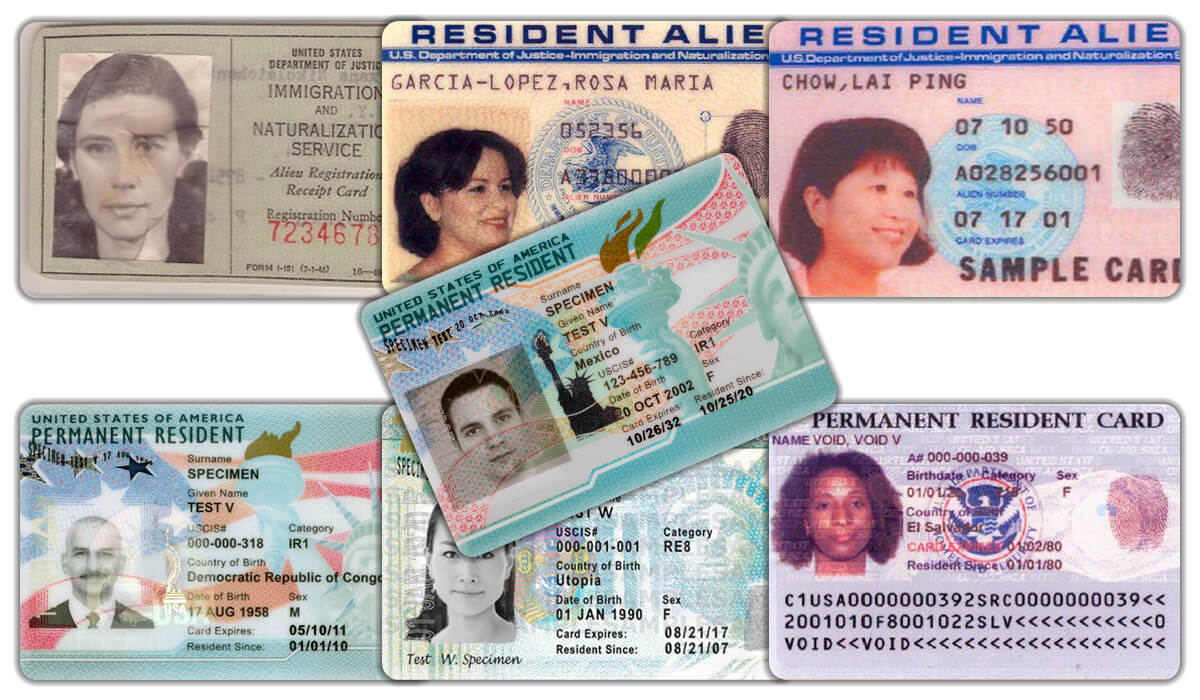
\includegraphics[width=0.50\textwidth]{green-card-history-collage.jpg}
    \caption[Evolución histórica de la Tarjeta de Residencia Permanente.]{Evolución histórica del diseño de la Tarjeta de Residencia Permanente de los Estados Unidos. El nombre coloquial \textit{Green Card} se origina en las versiones impresas en papel verde de la década de 1940. Adaptado de CitizenPath, ``History of the Green Card'' (2023) \cita{2}.}
    \label{fig:greencard_history}
\end{figure}

% NOTA: figura del anuncio presidencial de noviembre de 2025 retirada del cuerpo
% por considerarse políticamente sensible para una entrega académica. La cita
% [3] se conserva como referencia bibliográfica del evento mencionado en prosa.

Además de las restricciones estructurales derivadas de cuotas anuales y límites por país, el sistema migratorio opera en un entorno institucional sensible a cambios administrativos, anuncios de política pública y variaciones de demanda \cita{3} (véase Figura~\ref{fig:visabulletin}). Estos factores no se traducen necesariamente en efectos inmediatos o causales sobre el \textit{Visa Bulletin}, pero refuerzan la necesidad de modelos que reporten intervalos de predicción al 95\,\% y eviten presentar los pronósticos como certezas individuales. La magnitud agregada del rezago es ilustrativa. Para junio de 2025, el Servicio de Ciudadanía e Inmigración de los Estados Unidos (\textit{United States Citizenship and Immigration Services}, USCIS) reportó un rezago de 11.5 millones de casos pendientes \textbf{para todos los formularios de inmigración} (no exclusivamente \textit{Visa Bulletin}), con 5.4 millones que habían excedido los tiempos de procesamiento aceptables \cita{4}. La agencia completó 2.7 millones de casos en el segundo trimestre del año fiscal 2025, un 18\,\% menos que en el mismo periodo del año anterior \cita{5}. Del lado específico de visas familiares basadas en preferencia, FWD.us estima aproximadamente 4 millones de personas en espera consular \cita{6}; este último es el subconjunto directamente relacionado con el comportamiento del \textit{Visa Bulletin}. Cada caso pendiente representa un proceso individual con implicaciones familiares, laborales y financieras.

\begin{figure}[h!]
    \centering
    
\includegraphics[width=0.70\textwidth]{May26_VisaBulletin_FamilyTablaA_Sample.png}
    \caption[Visa Bulletin: Final Action Dates familiares, mayo 2026.]{Fragmento del \textit{Visa Bulletin} del Departamento de Estado de los Estados Unidos correspondiente a mayo de 2026, sección ``A. Final Action Dates for Family-Sponsored Preference Cases''. Se observa la posición diferenciada de México respecto al resto de áreas de cargabilidad, particularmente en las categorías F1, F2A, F2B, F3 y F4. Fuente: U.S. Department of State, Bureau of Consular Affairs \cita{7}.}
    \label{fig:visabulletin}
\end{figure}

Ante esta problemática, la Inteligencia Artificial y la analítica de datos pueden contribuir a convertir décadas de registros históricos en estimaciones acompañadas de intervalos de predicción al 95\,\%, sujetas a contraste empírico. Si bien existen plataformas comerciales que ofrecen estimaciones del \textit{Visa Bulletin}, estas operan como sistemas cerrados que no permiten la validación científica de sus resultados. Simultáneamente, la literatura académica ha demostrado la viabilidad de modelos lineales y de aprendizaje profundo para la predicción de fenómenos migratorios complejos \cita{8}--\cita{9}, pero no se identifican en la revisión preliminar propuestas que aborden de manera sistemática la predicción de las fechas de prioridad del \textit{Visa Bulletin} para múltiples combinaciones de categoría migratoria y país de cargabilidad. La presente propuesta no se limita a un solo país: aunque México funciona como caso piloto por la severidad y visibilidad de sus rezagos en categorías familiares, el diseño del sistema y de la base de datos se orienta a una estructura extensible por país y categoría, incluyendo otros países de alta demanda y categorías basadas en empleo cuando la disponibilidad histórica de datos permita una evaluación metodológicamente robusta.

El presente anteproyecto plantea el desarrollo de un sistema predictivo abierto, transparente y empíricamente evaluable, orientado a estimar el comportamiento futuro de las fechas del \textit{Visa Bulletin}. \textbf{El objetivo general del proyecto es desarrollar un sistema predictivo aplicado} para las fechas de prioridad del \textit{U.S. Visa Bulletin}, organizado como panel multiserie por país o área de cargabilidad, categoría migratoria y tipo de tabla, que genere pronósticos mensuales a horizontes de 1, 3, 6 y 12 meses con intervalos de predicción al 95\,\%.

La importancia de la investigación se manifiesta en tres dimensiones complementarias. Desde una perspectiva \textbf{social}, el proyecto contribuye a la planificación informada de millones de solicitantes de residencia permanente que enfrentan tiempos de espera de hasta dos décadas, ofreciéndoles escenarios históricos y márgenes de incertidumbre comunicados de manera transparente. Desde una perspectiva \textbf{técnica}, aporta un marco abierto, reproducible y empíricamente evaluable que atiende limitaciones observables de las plataformas comerciales cerradas existentes ---particularmente la falta de transparencia sobre datos, metodología y protocolo de evaluación---, integrando modelos lineales clásicos y arquitecturas de aprendizaje profundo bajo un protocolo de validación temporal documentado. Desde una perspectiva \textbf{académica}, entrega una base de datos longitudinal abierta del \textit{Visa Bulletin} y un protocolo de evaluación trazable que habilitan futuras investigaciones sobre el comportamiento agregado del sistema migratorio estadounidense.

El documento se estructura en cuatro capítulos: el Capítulo~I presenta el planteamiento del problema con sus antecedentes, definición formal, objetivos y justificación; el Capítulo~II desarrolla el marco teórico y el marco tecnológico; el Capítulo~III describe el producto esperado y la forma de validación; y el Capítulo~IV detalla la metodología operativa, las fases de desarrollo y el cronograma de ejecución del proyecto.

\clearpage

% ============================================================
% I. PLANTEAMIENTO DEL PROBLEMA
% ============================================================
\chapter{I. Planteamiento del problema}

En este capítulo se presenta el planteamiento del problema que fundamenta el presente proyecto. Se abordan, en primer término, los antecedentes del sistema migratorio estadounidense y los estudios académicos previos relacionados con el modelado predictivo de datos migratorios. Posteriormente, se presenta la definición formal del problema, los objetivos del proyecto, las preguntas e hipótesis y la justificación.

\section{1.1 Antecedentes (Contexto y trabajos preliminares)}

El sistema migratorio de los Estados Unidos opera bajo la Ley de Inmigración y Nacionalidad (\textit{Immigration and Nationality Act}, INA) de 1965 \cita{10}, que estableció cuotas anuales y la restricción estatutaria del 7\,\% por país (\textit{per-country limit}) sobre el total de visas de preferencia familiar y laboral. El Departamento de Estado (\textit{Department of State}, DOS) publica mensualmente el \textit{Visa Bulletin} \cita{7} con las fechas de prioridad vigentes; sin embargo, la asimetría entre demanda creciente y cuotas inflexibles ha producido tiempos de espera superiores a dos décadas, particularmente para países de alta demanda como México, India, China y Filipinas \cita{6}. Para el tercer trimestre del año fiscal 2025, USCIS reportó un rezago neto (\textit{net backlog}) superior a 5.4~millones de casos que excedieron los tiempos de procesamiento establecidos \cita{4}, y cerca de 4~millones de personas permanecían en espera de una visa de base familiar \cita{6}.

El comportamiento mensual de las fechas publicadas es altamente irregular: una misma serie puede registrar avances de varios meses en una sola edición, periodos prolongados de estancamiento o retrocesos impredecibles conocidos como \textit{retrogresión} \cita{7}. A esto se suma la presencia de los códigos administrativos \textit{Current} (todos los solicitantes pueden avanzar) y \textit{Unavailable} (cupo agotado o congelamiento administrativo), que rompen la continuidad numérica de las series y combinan tramos continuos con regímenes administrativos categóricos.

La literatura revisada confirma que los fenómenos migratorios pueden abordarse mediante modelos de series temporales, aprendizaje automático y arquitecturas híbridas; sin embargo, los trabajos existentes se concentran en flujos migratorios agregados, clasificación de solicitudes individuales o predicción de asilo, y no en el comportamiento mensual de las fechas de prioridad del \textit{U.S. Visa Bulletin}. La Tabla~\ref{tab:antecedentes} sintetiza los antecedentes más relevantes y su utilidad para el presente proyecto.

\begin{table}[H]
    \centering
    \footnotesize
    \arrayrulecolor{uacjblue}
    \setlength{\arrayrulewidth}{0.7pt}
    \setlength{\tabcolsep}{4pt}
    \begin{tabular}{>{\raggedright\arraybackslash}p{3.0cm}
                    >{\raggedright\arraybackslash}p{4.2cm}
                    >{\raggedright\arraybackslash}p{5.6cm}}
        \hline
        \rowcolor{uacjblue!85}
        \textcolor{white}{\textbf{Fuente}} &
        \textcolor{white}{\textbf{Técnica o enfoque}} &
        \textcolor{white}{\textbf{Utilidad para el proyecto}} \\
        \hline
        \rowcolor{uacjblue!4}
        Fabio \cita{8} & Series de tiempo e intervención sobre datos de inmigración EE.\,UU. (1820--2020) & Evidencia que los datos migratorios pueden analizarse como procesos temporales con cambios estructurales. \\
        Vegesana \cita{11} & Modelos supervisados (Naïve Bayes, regresión logística, Bosques Aleatorios) sobre peticiones H-1B & Demuestra la aplicabilidad del aprendizaje automático sobre datos migratorios estructurados. \\
        \rowcolor{uacjblue!4}
        Jain \textit{et al.} \cita{12} & Modelo híbrido ARIMA-LSTM con MAPE de 2.4\,\% & Antecedente técnico para combinar componentes lineales y no lineales en series complejas con retrogresiones. \\
        Carammia \textit{et al.} \cita{13} & ML adaptativo con registros administrativos y fuentes externas para flujos de asilo en la UE & Justifica el uso de datos administrativos para anticipar fenómenos migratorios. \\
        \rowcolor{uacjblue!4}
        Pu \textit{et al.} \cita{9} & Revisión sistemática sobre IA aplicada a la migración & Respalda la pertinencia de superar modelos econométricos aislados con técnicas de Inteligencia Artificial (IA). \\
        VisaBulletin.ai & Plataforma comercial cerrada con metodología, datos y protocolo de evaluación no publicados de forma auditable & Justifica la necesidad de una alternativa abierta, reproducible y auditable, dado que la plataforma no publica su metodología, datos ni protocolo de evaluación. \\
        \hline
    \end{tabular}
    \arrayrulecolor{black}
    \caption[Síntesis de antecedentes relevantes para el proyecto.]{Síntesis de los antecedentes más relevantes para el proyecto y su utilidad específica para el sistema predictivo del \textit{Visa Bulletin}. Fuente: elaboración propia.}
    \label{tab:antecedentes}
\end{table}

A partir de esta revisión se identifica una brecha: la ausencia, en la revisión preliminar, de un sistema abierto, reproducible y empíricamente evaluado para pronosticar fechas de prioridad por país o área de cargabilidad, categoría migratoria y tipo de tabla. La fuente primaria oficial, Travel.State.Gov, provee información mensual desde la década de 1980 \cita{7}, \cita{14} pero no ofrece herramientas analíticas ni predictivas; aunque existen boletines históricos previos a 1992, el proyecto acota la base longitudinal al periodo 1992--2026 por disponibilidad, consistencia estructural y suficiencia para construir series mensuales comparables. El proyecto aborda esta brecha integrando los datos tabulares históricos del \textit{Visa Bulletin} con modelos lineales clásicos y arquitecturas de aprendizaje profundo ---en particular la red recurrente LSTM como componente de un modelo híbrido--- para estimar rangos de fechas de prioridad útiles a la planificación de los solicitantes. La Figura~\ref{fig:greencard} ilustra el horizonte simbólico del proceso: la ceremonia de naturalización que culmina, años después de la obtención de la residencia permanente, el tránsito hacia la ciudadanía estadounidense.

\begin{figure}[H]
    \centering
    
\includegraphics[width=0.65\textwidth]{immigrants_citizenship.jpg}
    \caption[Ceremonia de naturalización de nuevos ciudadanos estadounidenses.]{Ceremonia de naturalización de nuevos ciudadanos estadounidenses. Fuente: The New York Times \cita{15}.}
    \label{fig:greencard}
\end{figure}

\section{1.2 Definición del problema}

Aunque el Departamento de Estado publica el \textit{Visa Bulletin} con cobertura mensual desde la década de 1980, el proyecto acota la base longitudinal al periodo 1992--2026 por disponibilidad, consistencia estructural y suficiencia para construir series mensuales comparables entre país de cargabilidad, categoría migratoria y tipo de tabla. Sobre ese alcance, \textbf{no se identificó, en la revisión preliminar, un sistema predictivo abierto, reproducible y empíricamente evaluado} que permita a los solicitantes estimar la evolución futura de las fechas de prioridad acompañando cada pronóstico con un intervalo de predicción al 95\,\%.

\textbf{La consecuencia directa} de esta ausencia es operativa: para los millones de solicitantes con peticiones aprobadas que aguardan una visa familiar (Sección~1.1), la imposibilidad de anticipar el comportamiento de las fechas de corte se traduce en decisiones diarias tomadas a ciegas: cuándo aceptar una promoción laboral, cuándo iniciar trámites educativos, cuándo planear una reunificación familiar.

\textbf{La necesidad} que aborda el presente proyecto es convertir más de tres décadas de datos públicos en un sistema que entregue pronósticos mensuales con intervalos de predicción al 95\,\% para los solicitantes y, simultáneamente, una base de datos abierta y auditable para futuras investigaciones académicas. Aunque en la literatura existen trabajos que aplican aprendizaje automático a datos migratorios \cita{8}--\cita{9} y herramientas comerciales que ofrecen estimaciones del \textit{Visa Bulletin}, ninguna de las propuestas identificadas integra de manera sistemática los datos históricos por país-categoría-tabla en un sistema con esas tres características conjuntas (apertura, reproducibilidad e incertidumbre cuantificada).

\section{1.3 Objetivos}

\subsection*{Objetivo General}

Desarrollar e implementar un sistema predictivo para series temporales del \textit{U.S. Visa Bulletin} que estime el comportamiento mensual de las fechas de prioridad por país o área de cargabilidad, categoría migratoria y tipo de tabla.

\subsection*{Objetivos Específicos}

Los cinco objetivos específicos se enuncian a continuación y se sintetizan visualmente en la Figura~\ref{fig:objetivos_visapredict}, donde cada tarjeta vincula el verbo de acción con su producto verificable y la fase metodológica correspondiente del Capítulo~IV.

\begin{enumerate}[label=\arabic*., leftmargin=1.2cm, itemsep=4pt]

    \item Construir la base de datos del \textit{U.S. Visa Bulletin} a partir de los boletines mensuales históricos.

    \item Caracterizar el comportamiento histórico de las series por país, categoría y tabla.

    \item Implementar y comparar modelos lineales y no lineales sobre el conjunto piloto evaluable.

    \item Evaluar el desempeño predictivo bajo validación temporal \textit{walk-forward}, con métricas robustas a escala e intervalos de predicción al 95\,\%.

    \item Entregar un demostrador académico que permita consultar series, pronósticos e intervalos por país y categoría.

\end{enumerate}

\begin{figure}[H]
    \centering
    \begin{tikzpicture}[
        font=\footnotesize,
        every node/.style={align=center, inner sep=0pt, outer sep=0pt},
        % ===== Geometría fija =====
        % Card: 2.85cm ancho × 5.4cm alto. Gap horizontal 0.20cm.
        % Total: 5*2.85 + 4*0.20 = 15.05cm (cabe en textwidth ~15.24cm)
        % Centros x: 1.425, 4.475, 7.525, 10.575, 13.625
        % ============= Estilos =============
        oecard/.style={rectangle, rounded corners=5pt, draw=uacjblue, line width=0.8pt,
                       fill=white, minimum width=2.85cm, minimum height=5.4cm,
                       anchor=north},
        oehead/.style={rectangle, rounded corners=5pt, fill=uacjblue, text=white,
                       minimum width=2.85cm, minimum height=1.05cm,
                       font=\Large\bfseries, anchor=north, inner sep=0pt},
        oeverb/.style={font=\scriptsize\bfseries, text=uacjblue, anchor=center,
                       minimum width=2.75cm, minimum height=0.55cm,
                       inner sep=2pt},
        oedesc/.style={text=uacjblack, font=\scriptsize, anchor=center,
                       text width=2.6cm, minimum height=2.05cm, align=center,
                       inner sep=2pt},
        oeprod/.style={rectangle, rounded corners=3pt, fill=uacjyellow!60,
                       draw=uacjblue!45, line width=0.4pt,
                       text=uacjblack, font=\scriptsize\bfseries,
                       minimum width=2.5cm, minimum height=0.85cm, anchor=center,
                       text width=2.35cm, align=center, inner sep=2pt},
        oefase/.style={font=\scriptsize\itshape, text=uacjgray, anchor=north,
                       minimum width=2.85cm, minimum height=0.4cm},
        oearrow/.style={-{Stealth[length=2.4mm,width=1.8mm]},
                        draw=uacjblue!55, line width=0.7pt},
        ogbanner/.style={rectangle, rounded corners=5pt, fill=uacjblue!8,
                         draw=uacjblue!55, line width=0.5pt,
                         minimum height=0.85cm, text=uacjblack,
                         font=\scriptsize, inner xsep=10pt, inner ysep=5pt,
                         text width=14.5cm, align=center}
    ]
        % ===== Banner OG =====
        \node[ogbanner] (og) at (7.525, 7.0)
            {\textbf{\textcolor{uacjblue}{OBJETIVO GENERAL:}} desarrollar e implementar un sistema predictivo para series temporales del \textit{U.S. Visa Bulletin} por país, categoría y tabla.};

        % ===== Cards =====
        % Layout vertical estricto interno (alturas relativas a card.north):
        %   Header (top → -1.05cm)
        %   Verbo  (centro a -1.55cm)
        %   Desc   (centro a -2.95cm, altura uniforme 2.05cm)
        %   Chip   (centro a -4.85cm, ancho uniforme 2.5cm)
        % Card.south = -5.4cm
        \foreach \i/\xc/\num/\verb/\desc/\prod/\fase in {%
            1/1.425/01/CONSTRUIR/{la base de datos histórica del \textit{Visa Bulletin}}/{$\blacktriangleright$\;CSV abierto}/Fase~1,
            2/4.475/02/CARACTERIZAR/{el comportamiento de las series por país, categoría y tabla}/{$\blacktriangleright$\;EDA + reportes}/Fase~2,
            3/7.525/03/IMPLEMENTAR/{modelos lineales y no lineales sobre el piloto evaluable}/{$\blacktriangleright$\;Modelos entrenados}/Fase~3,
            4/10.575/04/EVALUAR/{el desempeño bajo \textit{walk-forward} con intervalos al 95\,\%}/{$\blacktriangleright$\;Reporte de evaluación}/Fase~4,
            5/13.625/05/ENTREGAR/{el demostrador de visualización por país y categoría}/{$\blacktriangleright$\;App ejecutable}/Fase~5%
        }{
            \node[oecard] (c\i) at (\xc, 5.4) {};
            \node[oehead] at (c\i.north) {\num};
            \node[oeverb] at ([yshift=-1.55cm]c\i.north) {\verb};
            \node[oedesc] at ([yshift=-2.95cm]c\i.north) {\desc};
            \node[oeprod] at ([yshift=-4.80cm]c\i.north) {\prod};
            \node[oefase] at ([yshift=-1mm]c\i.south) {\fase};
        }

        % ===== Líneas punteadas del banner OG hacia los extremos =====
        \draw[uacjblue!35, line width=0.45pt, dashed]
            (og.south) -- ++(0,-0.25) -| (c1.north);
        \draw[uacjblue!35, line width=0.45pt, dashed]
            (og.south) -- ++(0,-0.25) -| (c5.north);
    \end{tikzpicture}
    \caption[Hoja de ruta de los Objetivos Específicos del proyecto.]{Hoja de ruta de los cinco Objetivos Específicos del proyecto. Cada tarjeta enuncia el verbo de acción, el contenido del objetivo, el producto verificable que entrega y la fase metodológica del Capítulo~IV en la que se desarrolla. Fuente: elaboración propia.}
    \label{fig:objetivos_visapredict}
\end{figure}

\section{1.4 Justificación}

\subsection*{Justificación social}

El proyecto se justifica socialmente porque las fechas de prioridad del \textit{Visa Bulletin} inciden en decisiones familiares, laborales, educativas y financieras de millones de solicitantes de residencia permanente; tan sólo cerca de cuatro millones de personas aguardan una visa de base familiar dentro de un rezago global del USCIS que excedió los 5.4~millones de casos en el tercer trimestre del año fiscal 2025 \cita{4}, \cita{6}. La incertidumbre sobre el avance, estancamiento o retroceso de las fechas dificulta la planeación individual, como ilustra la Figura~\ref{fig:visa_bulletin} para las categorías de preferencia familiar de México \cita{7}, \cita{14}. Aunque el sistema propuesto no elimina la incertidumbre migratoria ni sustituye asesoría legal, sí puede contribuir a comunicar escenarios históricos y márgenes de incertidumbre de forma más clara, abierta y verificable que las herramientas cerradas que operan actualmente en este dominio.

\begin{figure}[H]
    \centering
    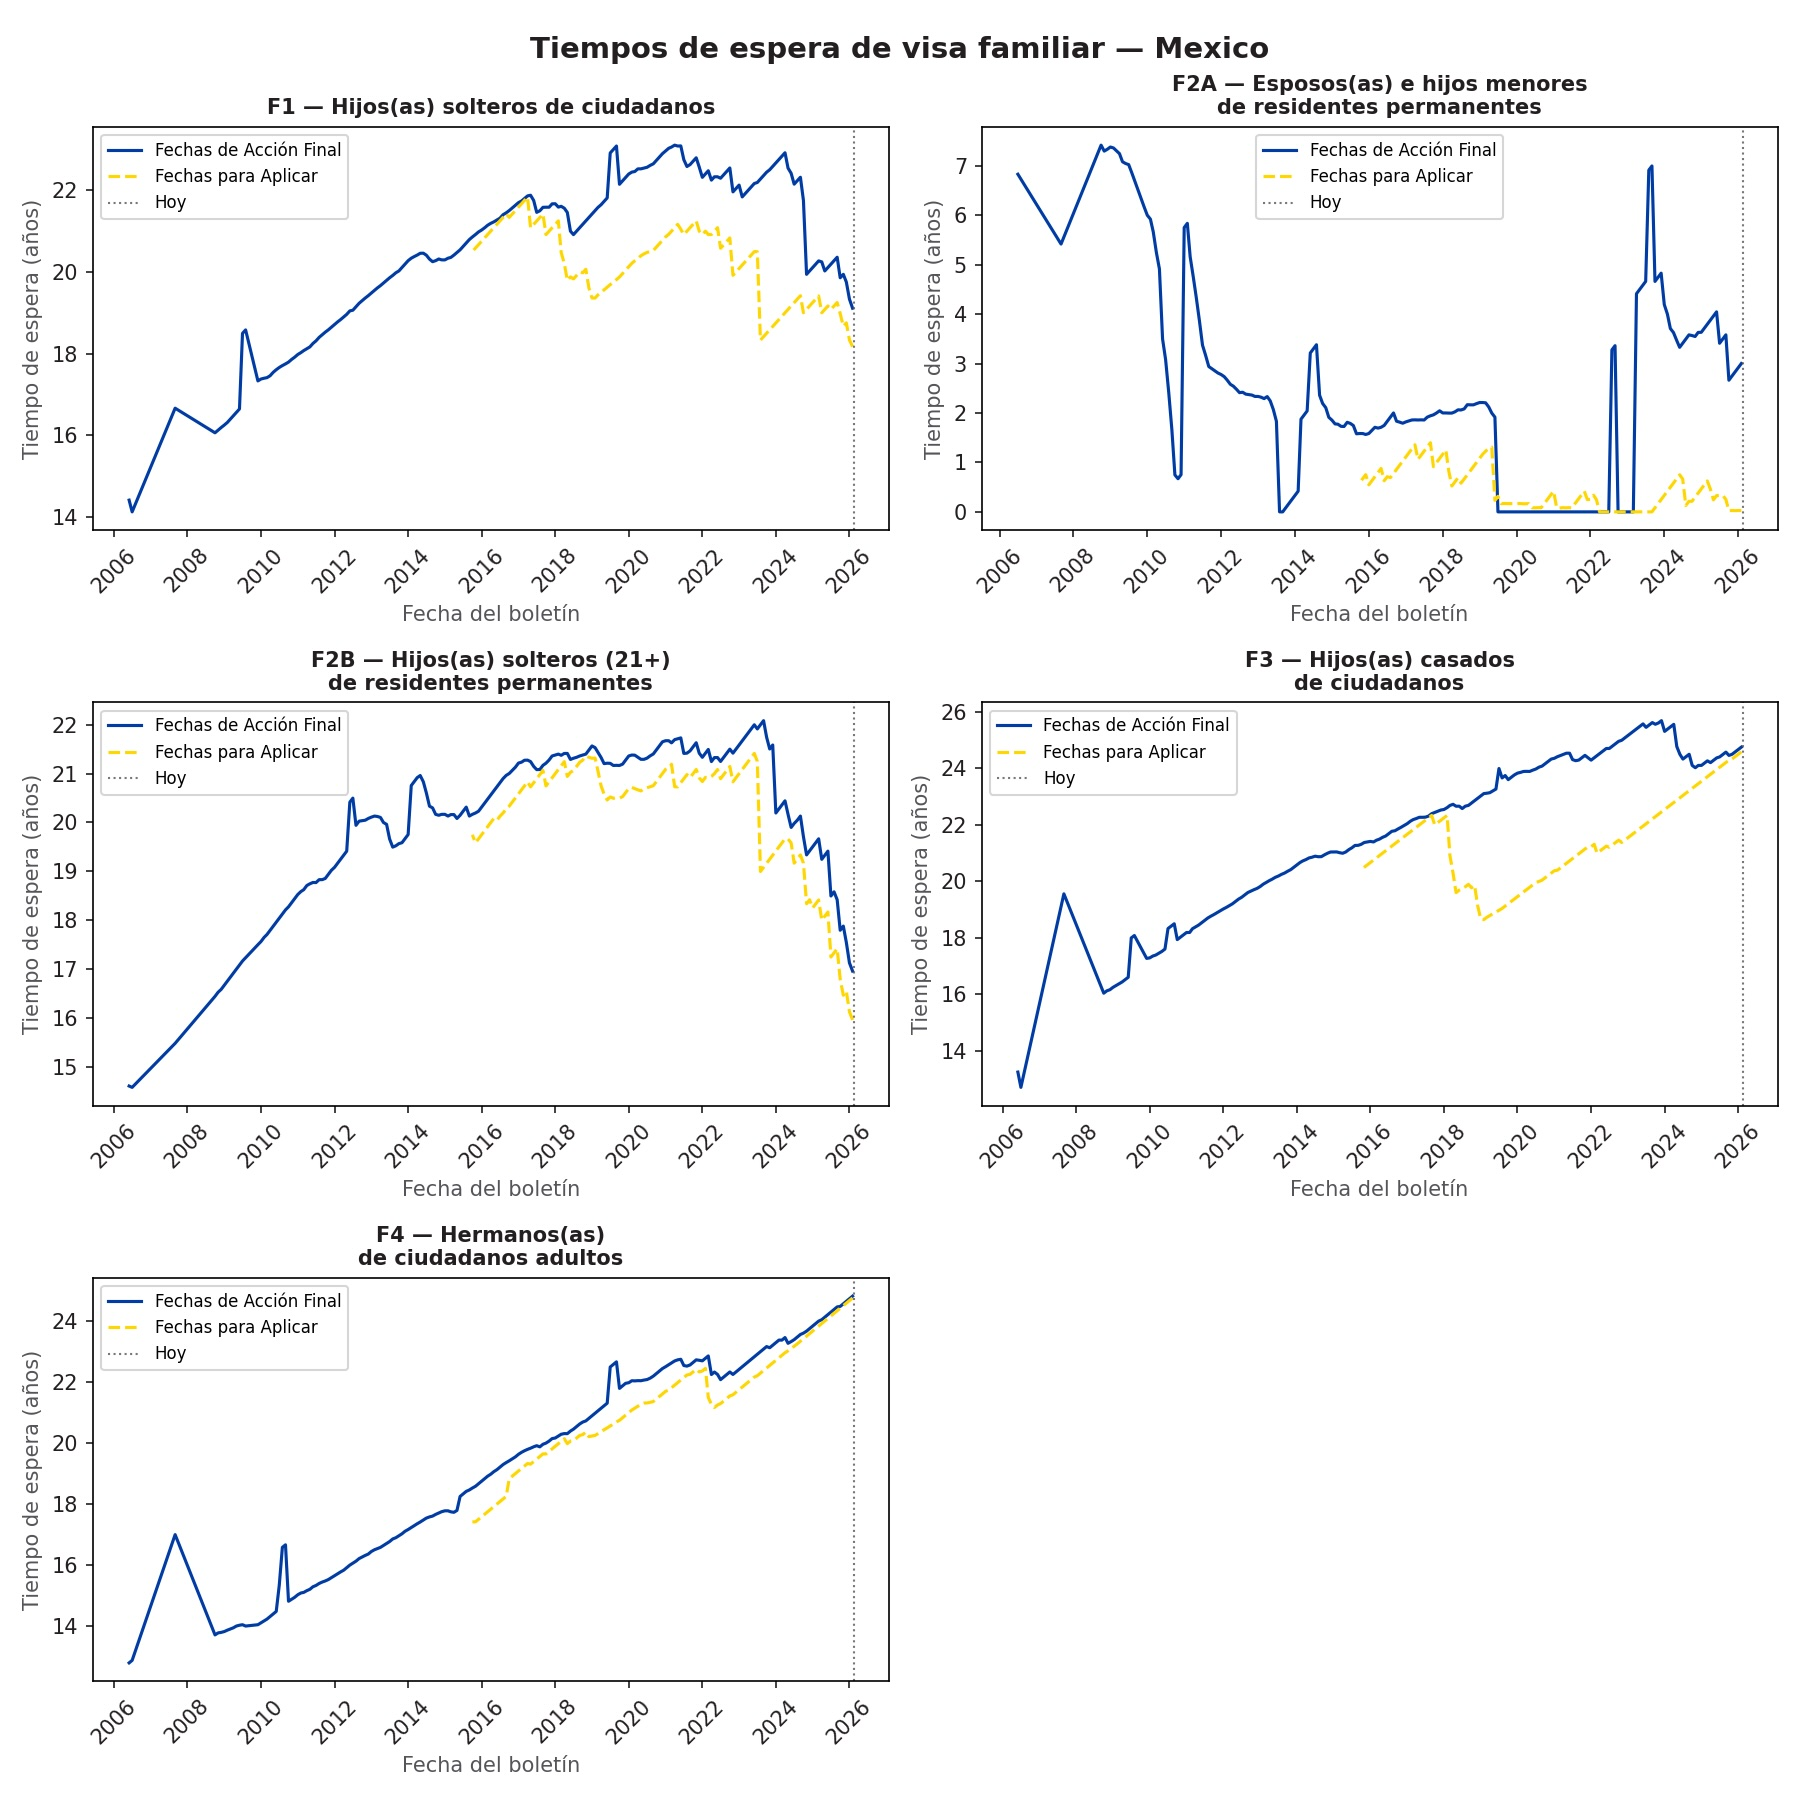
\includegraphics[width=0.85\textwidth]{Mexico_family_visa_wait_times.jpg}
    \caption[Tiempos de espera históricos de visa familiar para México (2006--2026).]{Tiempos de espera históricos de visa familiar para México, categorías F1, F2A, F2B, F3 y F4 (2006--2026). México se utiliza como ejemplo ilustrativo de país o área de cargabilidad de alta demanda y rezagos severos. Fuente: elaboración propia con datos del Departamento de Estado \cita{7}, \cita{14}.}
    \label{fig:visa_bulletin}
\end{figure}

\subsection*{Justificación técnica}

Desde el punto de vista técnico, el \textit{Visa Bulletin} constituye un problema relevante de modelado temporal porque combina fechas numéricas, estados administrativos categóricos (\textit{Current} y \textit{Unavailable}), periodos de estancamiento y episodios de retrogresión. Esta estructura exige comparar modelos lineales y no lineales bajo validación temporal \textit{walk-forward} con métricas robustas a escala e intervalos de predicción \cita{16}, \cita{17}, \cita{18}, evitando asumir de antemano que una arquitectura compleja será superior. La hibridación ARIMA-LSTM y los modelos globales como DeepAR cuentan con precedentes documentados en otros dominios \cita{12}, \cita{19}, \cita{20}--\cita{21}, \cita{22}; la aportación técnica de este trabajo no radica en proponer una arquitectura inédita, sino en \textbf{aplicar e integrar correctamente esas técnicas al \textit{Visa Bulletin}} a partir de una base de datos estructurada, un protocolo de evaluación reproducible y la cuantificación explícita de la incertidumbre del pronóstico.

\subsection*{Justificación profesionalizante}

En términos profesionalizantes, el proyecto culmina en \textbf{tres productos tangibles}: una base de datos longitudinal del \textit{Visa Bulletin}, un sistema predictivo reproducible y un demostrador académico de visualización (descritos en el Capítulo~III). Estos entregables permiten trasladar conocimientos de inteligencia artificial, analítica de datos y evaluación de modelos a una solución aplicada, verificable y útil para explorar escenarios de planeación. De esta manera, el anteproyecto mantiene el perfil aplicado propio de la MIAAD y evita presentar el marco metodológico como producto final independiente; el impacto inmediato es informativo (apoyar la planificación de los solicitantes con intervalos de predicción al 95\,\%) y el impacto secundario es habilitar investigaciones académicas posteriores sobre el comportamiento agregado del sistema migratorio estadounidense.

\clearpage

% ============================================================
% 1.5 PREGUNTAS E HIPÓTESIS DE INVESTIGACIÓN
% ============================================================
\section{1.5 Preguntas e hipótesis}

Las preguntas e hipótesis aquí formuladas se derivan de los objetivos específicos de la Sección~1.3 y son evaluables con los datos, modelos y métricas descritos en el Capítulo~III. Las preguntas se enuncian en forma abierta; las hipótesis se contrastarán empíricamente con los datos del piloto.

\subsection*{Pregunta general}

\textit{¿De qué manera y con qué grado de precisión un sistema predictivo basado en modelos lineales y de aprendizaje profundo puede estimar el comportamiento mensual de las fechas de prioridad del \textit{U.S. Visa Bulletin}, por país o área de cargabilidad, categoría migratoria y tipo de tabla, bajo validación temporal \textit{walk-forward}?}

\subsection*{Preguntas específicas}

\begin{enumerate}[label=PE\arabic*., leftmargin=1.4cm, itemsep=4pt]
    \item \textbf{Caracterización histórica.} ¿Qué patrones de avance, estancamiento, retrogresión y de los códigos administrativos \textit{Current} y \textit{Unavailable} se observan en las series del \textit{Visa Bulletin} por país y categoría?
    \item \textbf{Desempeño predictivo.} ¿Qué modelo de los implementados ---lineales (ARIMA, SARIMA, Prophet) o no lineales (LSTM, ARIMA-LSTM, DeepAR, XGBoost)--- ofrece el mejor desempeño predictivo en sMAPE y MASE sobre el conjunto piloto evaluable, y con qué consistencia entre estratos?
    \item \textbf{Heterogeneidad predictiva.} ¿Qué características de las series (longitud efectiva, frecuencia de \textit{Current}/\textit{Unavailable}, presencia de retrogresiones) están asociadas con mayor dificultad predictiva del sistema?
    \item \textbf{Calibración de incertidumbre.} ¿Qué cobertura empírica alcanzan los intervalos de predicción al 95\,\% generados por el sistema, y cómo varía esa cobertura entre estratos país-categoría-tabla?
\end{enumerate}

\subsection*{Hipótesis}

\begin{enumerate}[label=H\arabic*., leftmargin=1.2cm, itemsep=4pt]
    \item \textbf{Desempeño predictivo.} Se espera que el mejor modelo no lineal del marco comparativo (ARIMA-LSTM, DeepAR o XGBoost) reduzca el error de pronóstico (MASE) respecto al modelo lineal más fuerte en una proporción material de las series piloto evaluables. La identidad del modelo ganador es una pregunta empírica que el experimento responderá con datos.
    \item \textbf{Heterogeneidad estructural y calibración.} La dificultad predictiva ---medida como MASE del modelo ganador--- estará negativamente asociada a la longitud efectiva de la serie y positivamente asociada a la frecuencia de retrogresiones y transiciones C/U. Adicionalmente, los intervalos de predicción al 95\,\% alcanzarán una cobertura empírica cercana a la nominal en el agregado, con posibles desviaciones en estratos administrativos inestables.
\end{enumerate}

Estas hipótesis postulan asociaciones predictivas verificables empíricamente con los datos del proyecto; no asumen relaciones causales entre las decisiones administrativas del Departamento de Estado y los regresores empleados. La interpretación causal queda explícitamente fuera del alcance del proyecto.

\clearpage

% ============================================================
% II. MARCO TEÓRICO Y TECNOLÓGICO (v4.0 — subsecciones numeradas)
% ============================================================
\chapter{II. Marco Teórico y Tecnológico}

En este capítulo se desarrollan los fundamentos teóricos y las herramientas tecnológicas que sustentan el sistema predictivo propuesto. La Sección~2.1 expone el marco teórico, organizado en ocho subsecciones que cubren el sistema migratorio estadounidense y el \textit{Visa Bulletin} (2.1.1), las series de tiempo y los modelos lineales clásicos (2.1.2), los fundamentos del aprendizaje profundo (2.1.3), las redes neuronales recurrentes y la arquitectura LSTM (2.1.4), los modelos híbridos y las arquitecturas modernas de pronóstico (2.1.5), el aprendizaje automático aplicado a fenómenos migratorios (2.1.6), las métricas y los protocolos de evaluación de modelos predictivos (2.1.7) y, finalmente, el pronóstico multiserie y la heterogeneidad estructural por país-categoría (2.1.8). La Sección~2.2 describe el marco tecnológico organizado en cinco subsecciones operativas. Cada subsección teórica concluye con un párrafo de \textit{Implicación para este proyecto} que conecta el contenido con una decisión metodológica concreta del Capítulo~III.

\section{2.1 Fundamentos teóricos}

\subsection{2.1.1 El sistema de inmigración de Estados Unidos y el \textit{Visa Bulletin}}

El sistema de inmigración basado en preferencias de los Estados Unidos tiene su origen en la \textit{Immigration and Nationality Act} (INA) de 1965, legislación que reemplazó el sistema de cuotas por origen nacional vigente desde 1921 e introdujo un esquema de categorías de preferencia con límites numéricos anuales \cita{10}. La INA, codificada en el Título 8 del \textit{U.S. Code} (\S\S\,1151--1153), establece en su Sección 201 un mínimo anual de 226,000 visas de inmigrante por preferencia familiar y 140,000 por preferencia laboral, para un techo global de aproximadamente 675,000 admisiones permanentes anuales, excluyendo familiares inmediatos de ciudadanos, refugiados y asilados \cita{10}. La Sección 202 de la INA prescribe un \textbf{límite por país del 7\,\%} del total combinado de visas familiares y laborales, equivalente a un máximo de aproximadamente 25,620 visas anuales por nación independiente, disposición que constituye la causa estructural primaria del rezago migratorio (\textit{backlog}) que afecta desproporcionadamente a países con alta demanda como India, China, México y Filipinas \cita{23}.

Las categorías de preferencia familiar, definidas en la Sección 203(a) de la INA, se organizan en cinco niveles \cita{10}, \cita{7}. La categoría \textbf{F1} corresponde a hijos e hijas solteros mayores de 21 años de ciudadanos estadounidenses, con una asignación de 23,400 visas anuales. La categoría \textbf{F2} se subdivide en \textbf{F2A}, para cónyuges e hijos menores de 21 años de residentes permanentes legales (\textit{Lawful Permanent Residents}, LPR), que recibe el 77\,\% de las 114,200 visas asignadas a F2, y \textbf{F2B}, para hijos solteros mayores de 21 años de LPR, que recibe el 23\,\% restante. A lo largo del documento, la convención \textbf{F1--F4} se utiliza como abreviatura del conjunto completo \{F1, F2A, F2B, F3, F4\} (cinco series mensuales por país de cargabilidad), no como rango excluyente de F2A o F2B. La categoría \textbf{F3} comprende hijos casados de ciudadanos con 23,400 visas, mientras que \textbf{F4} abarca hermanos de ciudadanos adultos con 65,000 visas anuales. En el ámbito laboral, las categorías basadas en empleo (\textit{Employment-Based}, EB) distribuyen las 140,000 visas anuales en cinco niveles: \textbf{EB-1} para trabajadores prioritarios, \textbf{EB-2} para profesionales con grados avanzados o capacidad excepcional, \textbf{EB-3} para trabajadores calificados y profesionales, \textbf{EB-4} para inmigrantes especiales y \textbf{EB-5} para inversionistas, cada uno con porcentajes definidos del total \cita{10}.

El \textit{Visa Bulletin}, publicado mensualmente por la Oficina de Asuntos Consulares del DOS, constituye el instrumento administrativo que regula la disponibilidad de números de visa \cita{7}. Desde octubre de 2015, el boletín presenta dos tablas: las \textbf{Final Action Dates} (FAD, Fechas de Acción Final), que determinan cuándo una visa puede ser efectivamente emitida, y las \textbf{Dates for Filing} (DFF, Fechas para Presentación), fechas más permisivas que indican cuándo un solicitante puede presentar documentación ante el \textit{National Visa Center} (NVC) o el formulario I-485 de ajuste de estatus \cita{7}. La \textbf{fecha de prioridad} (\textit{priority date}) de cada solicitante, definida como la fecha en que el USCIS recibe la petición de inmigrante (formulario I-130 para familiares o I-140 para empleo), establece su posición cronológica en la cola de espera. Las visas se asignan estrictamente en orden cronológico de fecha de prioridad dentro de cada categoría y país o área de cargabilidad, conforme a la Sección 203(e) de la INA.

El fenómeno de \textbf{retrogresión} ocurre cuando las fechas de corte en el \textit{Visa Bulletin} retroceden de un mes al siguiente, situación que deja a solicitantes previamente elegibles sin acceso temporal al siguiente paso de su trámite \cita{7}. Este fenómeno se origina cuando la demanda de números de visa en una categoría o país excede la oferta mensual disponible, forzando al DOS a restringir las fechas para mantener la emisión dentro de los límites anuales. La retrogresión es más frecuente hacia el final del año fiscal federal (julio--septiembre) y puede ser dramática: Bier \cita{23} documenta que las categorías basadas en empleo de países sujetos a límite efectivo, en particular India, han experimentado retrogresiones de varios años en periodos recientes en respuesta a desbalances entre demanda agregada y cuotas estatutarias.

La magnitud del rezago migratorio es considerable. Según datos compilados por FWD.us a partir de estadísticas del Departamento de Estado, aproximadamente 4 millones de personas esperan en el extranjero en filas de inmigración familiar \cita{6}. Bier \cita{23} documentó que los tiempos de espera promedio se duplicaron entre 1991 y 2018, pasando de 2 años y 10 meses a 5 años y 8 meses, con el 28\,\% de los inmigrantes esperando una década o más. El rezago total creció de aproximadamente 3.3 millones en 1992 a 6.9 millones en 2021, y se estima que 675,000 solicitantes (14\,\%) fallecerían antes de recibir su residencia permanente si permanecieran indefinidamente en la fila \cita{23}. Este fenómeno genera series de tiempo con características únicas: movimientos no lineales, retrogresiones abruptas, patrones estacionales ligados al calendario fiscal federal y dependencias estructurales de la política migratoria, lo que justifica la exploración de modelos predictivos avanzados que trasciendan los enfoques lineales tradicionales.

\paragraph{Consideración ética.} El despliegue de sistemas de inteligencia artificial en dominios con impacto directo sobre personas migrantes demanda transparencia metodológica, comunicación responsable de la incertidumbre y accesibilidad. El presente sistema no toma decisiones automáticas que afecten el estatus migratorio de individuos: se limita a pronosticar fechas oficiales publicadas por el gobierno estadounidense, publica código y datos abiertos, acompaña sus pronósticos con intervalos de predicción, y exhibe en el demostrador una advertencia explícita de que las estimaciones son informativas y no constituyen asesoría legal individual.

\paragraph{Implicación para este proyecto.} La estructura legal de la INA ---categorías de preferencia, cupos anuales, límite del 7\,\% por país y dos tablas (FAD y DFF)--- determina directamente la unidad de análisis del sistema. Cada combinación de país de cargabilidad, categoría migratoria y tipo de tabla define una serie temporal mensual con régimen propio. Esto sustenta la formulación de la variable predicha $y_{p,c,b,t}$ ---donde $p$ indexa el país o área de cargabilidad, $c$ la categoría migratoria, $b$ el tipo de tabla y $t$ el mes calendario--- como variable numérica continua sobre cada combinación (Sección~3.1.4), y la cobertura escalonada en estructural\,/\,evaluable\,/\,piloto (Tabla~\ref{tab:cobertura_visapredict}).

\subsection{2.1.2 Series de tiempo: fundamentos matemáticos y modelos clásicos}

Una \textbf{serie de tiempo} es la realización de un proceso estocástico $\{Y_t : t \in T\}$, donde $Y_t$ es el valor observado en el instante $t$ y $T = \{1, 2, \ldots\}$ es el conjunto de instantes discretos \cita{24}, \cita{25}; el análisis busca identificar su estructura de dependencia temporal para describirla y pronosticarla. La \textbf{descomposición clásica} representa la serie en forma aditiva $Y_t = T_t + S_t + C_t + \varepsilon_t$ \cita{24}, \cita{26}, donde $T_t$ es la componente de tendencia (movimiento sistemático de largo plazo), $S_t$ la componente estacional (oscilaciones de período fijo), $C_t$ la componente cíclica (oscilaciones de período variable, no necesariamente fijo) y $\varepsilon_t$ el componente irregular o ruido aleatorio sin estructura predecible. El supuesto de \textbf{estacionariedad débil} (media, varianza y autocovarianza independientes del tiempo) se contrasta empíricamente con dos pruebas de hipótesis con criterios opuestos, lo que provee confirmación cruzada robusta: la prueba \textbf{Augmented Dickey-Fuller} (ADF) \cita{27} ---prueba de raíz unitaria cuya hipótesis nula es la no estacionariedad; rechazarla sugiere que la serie es estacionaria--- y la prueba \textbf{Kwiatkowski-Phillips-Schmidt-Shin} (KPSS) \cita{28} ---con hipótesis nula opuesta: la serie es estacionaria; rechazarla sugiere no estacionariedad---. La estructura de dependencia temporal se identifica con la función de \textbf{autocorrelación} (ACF), que cuantifica la correlación entre observaciones separadas por $k$ rezagos, y la función de \textbf{autocorrelación parcial} (PACF), que mide esa correlación eliminando el efecto lineal de los rezagos intermedios; el patrón conjunto de ACF y PACF orienta la selección del orden $(p, q)$ del modelo bajo la metodología iterativa de \textbf{Box-Jenkins} \cita{24}, \cita{29}.

Los \textbf{modelos ARIMA} (\textit{AutoRegressive Integrated Moving Average}) \cita{24}, \cita{29} son la piedra angular del pronóstico clásico. El modelo ARIMA$(p,d,q)$ se expresa, en notación de operador de retardo $B$ con $BY_t = Y_{t-1}$, como
\begin{equation}
    \phi_p(B)(1-B)^d Y_t = c + \theta_q(B)\varepsilon_t,
\end{equation}
donde $\phi_p(B)$ y $\theta_q(B)$ son los polinomios autorregresivo y de media móvil (de órdenes $p$ y $q$) en el operador $B$, $d$ es el grado de diferenciación, $c$ una constante y $\varepsilon_t$ el ruido blanco. Su extensión estacional \textbf{SARIMA} (\textit{Seasonal ARIMA}) $(p,d,q)(P,D,Q)_s$ \cita{29} incorpora componentes estacionales multiplicativos de período $s$, donde $(P, D, Q)$ son las versiones estacionales de los órdenes $(p, d, q)$; la extensión \textbf{ARIMAX} permite incluir regresores exógenos contemporáneos como indicadores de política migratoria o calendarios fiscales \cita{29}. La selección de órdenes sigue Box-Jenkins guiada por los criterios de información de Akaike (\textit{Akaike Information Criterion}, AIC) \cita{30} y bayesiano (\textit{Bayesian Information Criterion}, BIC) \cita{31}; el BIC, más estricto con la complejidad, es preferible cuando el tamaño muestral $n$ es grande. Como alternativa, \textbf{Prophet} \cita{32} descompone la serie aditivamente con tendencia por tramos, estacionalidad de Fourier y efectos de calendario explícitos, sacrificando rigurosidad estadística por robustez ante atípicos y facilidad de uso.

Estos modelos, pese a su elegancia, son intrínsecamente lineales \cita{19}; Kontopoulou \textit{et al.} \cita{33} documentan que los enfoques de aprendizaje profundo mejoran la precisión hasta en 14\,\% frente a ARIMA, particularmente en predicciones de múltiples pasos, lo que motiva la exploración de arquitecturas híbridas.

\paragraph{Implicación para este proyecto.} ARIMA, SARIMA, ARIMAX y Prophet \cita{32} son los modelos lineales de referencia que los modelos no lineales del marco comparativo deberán superar (Sección~3.3.1) para satisfacer los criterios cualitativos de éxito. El BIC guía la selección del orden $(p,d,q)(P,D,Q)_s$ y la componente lineal del híbrido ARIMA-LSTM se construye con esta familia, absorbiendo con pocos parámetros la dinámica explicable de las series del \textit{Visa Bulletin}.

\subsection{2.1.3 Fundamentos del aprendizaje profundo}

El aprendizaje profundo es una familia de métodos basados en la composición jerárquica de representaciones no lineales mediante redes neuronales de múltiples capas \cita{34}, \cita{35}. Una \textbf{red neuronal artificial} compone capas $\mathbf{h}^{(\ell)} = \phi^{(\ell)}(\mathbf{W}^{(\ell)}\mathbf{h}^{(\ell-1)} + \mathbf{b}^{(\ell)})$ donde $\phi$ es una función de activación no lineal y $\mathbf{W}, \mathbf{b}$ son los parámetros entrenables; la versión clásica con $L$ capas, denominada \textbf{perceptrón multicapa} (MLP), puede representar funciones continuas arbitrarias dada suficiente capacidad por el teorema de aproximación universal \cita{34}. El entrenamiento minimiza una función de pérdida (típicamente MSE para regresión) mediante variantes del descenso del gradiente estocástico, con gradientes calculados por \textbf{retropropagación} \cita{36}.

El proyecto se apoya en tres elementos prácticos de esta familia: (i)~la activación \textbf{ReLU} (\textit{Rectified Linear Unit}) $\max(0, x)$ que mitiga el desvanecimiento del gradiente sufrido por las activaciones sigmoide y tanh \cita{37}; (ii)~el optimizador \textbf{Adam} de Kingma y Ba \cita{38}, estándar \textit{de facto} en redes profundas modernas, con valores $\beta_1 = 0.9$ y $\beta_2 = 0.999$ salvo refinamiento por búsqueda restringida; y (iii)~estrategias de regularización indispensables en régimen de datos pequeño ---\textit{weight decay}, \textbf{dropout} de Srivastava \textit{et al.} \cita{39}, su variante recurrente variacional de Gal y Ghahramani \cita{40}, normalización por lotes de Ioffe y Szegedy \cita{41} y \textit{early stopping} sobre el error de validación.

\paragraph{Implicación para este proyecto.} El régimen de datos pequeño ($\sim$290 observaciones por serie en FAD, $\sim$125 en DFF) hace inviable una red profunda sin contención agresiva. El entrenamiento del componente LSTM aplicará Adam con búsqueda restringida de hiperparámetros, \textit{dropout} (incluido el variacional \cita{40} para la cuantificación de incertidumbre), \textit{early stopping} y normalización por lotes.

\subsection{2.1.4 Redes neuronales recurrentes y arquitectura LSTM}

Las \textbf{redes neuronales recurrentes} (RNN) incorporan conexiones cíclicas que mantienen un estado oculto $\mathbf{h}_t = \phi(\mathbf{W}_{hh}\mathbf{h}_{t-1} + \mathbf{W}_{xh}\mathbf{x}_t + \mathbf{b}_h)$ ---donde $\mathbf{W}_{hh}$ es la matriz de pesos recurrentes (estado oculto a estado oculto), $\mathbf{W}_{xh}$ la matriz de pesos de entrada (entrada a estado oculto), $\mathbf{b}_h$ el vector de sesgo, $\mathbf{x}_t$ la entrada en el paso $t$ y $\phi$ la función de activación---, con función de pérdida ajustada por \textit{Backpropagation Through Time} (BPTT) \cita{42}, \cita{34}, \cita{36}. Su limitación principal es el \textbf{gradiente desvaneciente} demostrado por Bengio, Simard y Frasconi \cita{37}: durante la retropropagación a través de muchos pasos temporales, el producto repetido de pesos menores a uno hace que la señal de gradiente decrezca exponencialmente, impidiendo aprender dependencias de largo plazo (su contraparte, el \textit{gradiente explosivo}, se mitiga con recorte).

La arquitectura \textbf{Long Short-Term Memory} (LSTM) \cita{43} resuelve el desvanecimiento mediante un \textbf{estado de celda} $\mathbf{C}_t$ regulado por compuertas multiplicativas que permite el flujo de gradiente sin degradación. Las ecuaciones de una celda LSTM, dadas $\mathbf{x}_t$, $\mathbf{h}_{t-1}$ y $\mathbf{C}_{t-1}$, son:

\begin{align}
    \mathbf{f}_t &= \sigma(\mathbf{W}_f [\mathbf{h}_{t-1}, \mathbf{x}_t] + \mathbf{b}_f) & \text{(compuerta de olvido)}\\
    \mathbf{i}_t &= \sigma(\mathbf{W}_i [\mathbf{h}_{t-1}, \mathbf{x}_t] + \mathbf{b}_i) & \text{(compuerta de entrada)}\\
    \tilde{\mathbf{C}}_t &= \tanh(\mathbf{W}_C [\mathbf{h}_{t-1}, \mathbf{x}_t] + \mathbf{b}_C) & \text{(estado candidato)}\\
    \mathbf{C}_t &= \mathbf{f}_t \odot \mathbf{C}_{t-1} + \mathbf{i}_t \odot \tilde{\mathbf{C}}_t & \text{(actualización de celda)}\\
    \mathbf{o}_t &= \sigma(\mathbf{W}_o [\mathbf{h}_{t-1}, \mathbf{x}_t] + \mathbf{b}_o) & \text{(compuerta de salida)}\\
    \mathbf{h}_t &= \mathbf{o}_t \odot \tanh(\mathbf{C}_t) & \text{(estado oculto)}
\end{align}

donde $\sigma$ es la sigmoide, $\tanh$ la tangente hiperbólica, $\odot$ el producto de Hadamard, y $\mathbf{W}, \mathbf{b}$ las matrices de pesos y vectores de sesgo de cada compuerta \cita{43}, \cita{34}. La actualización aditiva $\mathbf{C}_t = \mathbf{f}_t \odot \mathbf{C}_{t-1} + \mathbf{i}_t \odot \tilde{\mathbf{C}}_t$ es la clave del diseño: al ser aditiva (no multiplicativa), los gradientes fluyen sin desvanecerse a lo largo de muchos pasos temporales. Variantes relevantes incluyen LSTM bidireccional (BiLSTM) \cita{44}, \cita{45}, LSTM apilada multi-capa \cita{34}, \cita{46} y \textbf{GRU} (\textit{Gated Recurrent Unit}) de Cho \textit{et al.} \cita{47}, que fusiona las compuertas de entrada y olvido. Los hiperparámetros críticos ---ventana retrospectiva, número de capas, dimensión del estado oculto, tasa de aprendizaje, \textit{batch size} y \textit{dropout} recurrente--- se seleccionan típicamente con búsqueda en cuadrícula, aleatoria u optimización bayesiana sobre validación temporal \cita{48}.

\paragraph{Implicación para este proyecto.} La LSTM constituye el componente no lineal del híbrido ARIMA-LSTM y se evalúa también como modelo de referencia univariado puro (Tabla~\ref{tab:modelos_referencia}, fila ``LSTM puro'' \cita{43}). La separación explícita entre LSTM puro y ARIMA-LSTM permite estimar empíricamente cuánta de la mejora atribuible al híbrido proviene del componente recurrente y cuánta de la integración con la parte lineal.

\subsection{2.1.5 Modelos híbridos y arquitecturas modernas para pronóstico}

El \textbf{fundamento teórico de la hibridación} entre modelos lineales y no lineales fue formalizado por Zhang \cita{19}, quien propuso descomponer la serie como $y_t = L_t + N_t$, con $L_t$ capturado por ARIMA y $N_t$ por una red neuronal. La estrategia \textbf{secuencial} ajusta primero ARIMA, calcula los residuales $e_t = y_t - \hat{L}_t$ y los modela con una LSTM, reportando reducciones del error cuadrático medio de hasta 18.87\,\% frente a los modelos individuales \cita{19}. Existen además estrategias en \textbf{paralelo} (promedio ponderado de salidas independientes) y de \textbf{ensamble} (\textit{stacking}, promedio óptimo) \cita{49}; la competencia M4 con 100\,000 series y 61 métodos \cita{50} mostró que 12 de los 17 más precisos eran combinaciones, y el ganador ES-RNN de Smyl \cita{49} superó al mejor método de combinación de referencia por aproximadamente 10\,\% en sMAPE.

La evidencia reciente de modelos híbridos ARIMA-LSTM es favorable en epidemiología \cita{12}, \cita{21}, economía \cita{51}, energía \cita{52} y comercio \cita{20}, aunque las magnitudes de mejora varían por dominio, característica de la serie y modelo de referencia, lo que motiva la evaluación empírica en el dominio migratorio del presente proyecto sin asumirla de antemano. Entre las arquitecturas modernas se documentan N-BEATS \cita{53}, \textit{Temporal Fusion Transformer} (TFT) \cita{54}, PatchTST \cita{55} y \textbf{DeepAR} \cita{22} (LSTM probabilística autorregresiva con distribuciones predictivas completas); de éstas, DeepAR es la única que el proyecto incorpora al marco comparativo por su pertinencia multiserie (Sección~2.1.8). El detalle conceptual de TFT y PatchTST queda únicamente como referencia bibliográfica y entrada de glosario. Paralelamente, \textbf{XGBoost} de Chen y Guestrin \cita{56} se incorpora como modelo tabular con regresores rezagados, calendáricos y categóricos en la Tabla~\ref{tab:modelos_referencia}.

\paragraph{Implicación para este proyecto.} La hibridación ARIMA-LSTM en cascada (estrategia secuencial de Zhang \cita{19}) constituye uno de los candidatos del marco comparativo, junto con DeepAR global \cita{22} y XGBoost tabular \cita{56}, todos enumerados en la Tabla~\ref{tab:modelos_referencia}. La identidad del modelo no lineal con mejor desempeño es una pregunta empírica que el estudio responderá con datos, no un compromiso adoptado de antemano. La inclusión simultánea de modelos lineales fuertes (Prophet) y de candidatos no lineales heterogéneos (local, global, tabular) mitiga el sesgo de selección que aparecería al comparar sólo contra modelos de referencia débiles.

\subsection{2.1.6 Aprendizaje automático aplicado a fenómenos migratorios}

La aplicación de técnicas de aprendizaje automático a fenómenos migratorios constituye un campo emergente pero creciente en la intersección de la ciencia de datos y los estudios migratorios. Pu \textit{et al.} \cita{9} presentaron una revisión sistemática que concluyó que no existe un modelo universalmente óptimo para predicción migratoria y que la calidad de los datos constituye la restricción principal. Los autores identificaron que la creciente disponibilidad de datos de redes sociales ha habilitado aplicaciones de IA previamente imposibles y que la integración de modelos de aprendizaje automático con enfoques tradicionales ofrecerá avances significativos \cita{9}.

En el ámbito del pronóstico de flujos de asilo, Carammia, Iacus y Wilkin \cita{13} desarrollaron un algoritmo adaptativo (AdaENet) que integra estadísticas administrativas con fuentes de datos no tradicionales y demostraron que superó a los modelos ARIMA de referencia, particularmente durante periodos anómalos como la crisis migratoria europea. Hoffmann Pham y Luengo-Oroz \cita{57} propusieron un marco computacional para estructurar el problema de predicción de desplazamiento forzado, advirtiendo que los modelos más flexibles pueden sobreajustar datos de desplazamiento debido a su naturaleza irregular e influenciada por eventos discretos. Esta advertencia es particularmente pertinente para el presente proyecto, dado que las fechas del \textit{Visa Bulletin} son sensibles a eventos de política que pueden generar cambios estructurales en la dinámica de las series.

En el contexto específico de la inmigración estadounidense, Fabio \cita{8} aplicó análisis de intervención y agrupamiento de series de tiempo a datos de inmigración de EE.\,UU. desde 1820 hasta 2020, y Vegesana \cita{11} adoptó un enfoque de clasificación supervisada para predecir decisiones sobre solicitudes de visa H-1B con datos de 2011 a 2016. A pesar de la demanda práctica evidenciada por herramientas comerciales como VisaBulletin.ai y MyPriorityDate.com, \textbf{no se identificó, en la revisión preliminar, trabajo académico publicado que aplique modelos de aprendizaje automático específicamente al pronóstico de fechas de prioridad del \textit{Visa Bulletin}}, lo que constituye una brecha clara en la literatura revisada que el presente proyecto busca abordar.

\paragraph{Implicación para este proyecto.} La revisión preliminar no identifica trabajos académicos que apliquen sistemáticamente modelos predictivos al \textit{Visa Bulletin} en múltiples combinaciones país\,$\times$\,categoría\,$\times$\,tabla. Esta brecha sustenta la pertinencia del proyecto y motiva su pregunta general (Sección~1.5). La cautela documentada por Hoffmann Pham y Luengo-Oroz \cita{57} sobre el sobreajuste de modelos flexibles en datos migratorios orienta la elección del régimen de regularización del Capítulo~IV.

\subsection{2.1.7 Evaluación de modelos predictivos de series de tiempo}

La evaluación rigurosa de modelos predictivos requiere métricas cuantitativas estandarizadas, diseño experimental apropiado para datos temporales, comparación estadística contra modelos de referencia y cuantificación de la incertidumbre. Hyndman y Koehler \cita{16} realizaron un análisis crítico de las métricas de precisión de pronóstico y propusieron un marco que distingue entre errores dependientes de escala, errores porcentuales, errores relativos y errores escalados.

Las \textbf{métricas dependientes de escala} incluyen el \textbf{Error Absoluto Medio} (MAE):
\begin{equation}
    \text{MAE} = \frac{1}{n}\sum_{t=1}^{n}|y_t - \hat{y}_t|
\end{equation}
y la \textbf{Raíz del Error Cuadrático Medio} (RMSE):
\begin{equation}
    \text{RMSE} = \sqrt{\frac{1}{n}\sum_{t=1}^{n}(y_t - \hat{y}_t)^2}
\end{equation}
donde $y_t$ es el valor observado, $\hat{y}_t$ el valor predicho y $n$ el número de observaciones del conjunto evaluado \cita{16}, \cita{58}. El RMSE penaliza desproporcionadamente errores grandes debido a la operación cuadrática, haciéndolo sensible a valores atípicos. El \textbf{Error Absoluto Porcentual Medio} (MAPE):
\begin{equation}
    \text{MAPE} = \frac{100\%}{n}\sum_{t=1}^{n}\left|\frac{y_t - \hat{y}_t}{y_t}\right|
\end{equation}
permite comparaciones independientes de escala pero presenta degeneración cuando $y_t$ se aproxima a cero \cita{16}. El \textbf{MAPE Simétrico} (sMAPE):
\begin{equation}
    \text{sMAPE} = \frac{100\%}{n}\sum_{t=1}^{n}\frac{|y_t - \hat{y}_t|}{(|y_t| + |\hat{y}_t|)/2}
\end{equation}
aborda parcialmente la asimetría del MAPE y fue la métrica principal de la competencia M4 \cita{50}. Hyndman y Koehler \cita{16} propusieron el \textbf{Error Absoluto Escalado Medio} (MASE) como métrica universal:
\begin{equation}
    \text{MASE} = \frac{1}{n}\sum_{t=1}^{n}\frac{|y_t - \hat{y}_t|}{\dfrac{1}{n-m}\displaystyle\sum_{i=m+1}^{n}|y_i - y_{i-m}|}
\end{equation}
donde $m$ es el período estacional. Un MASE menor que 1 indica que el modelo supera al pronóstico naïve estacional \cita{16}.

El \textbf{diseño experimental} para evaluación de modelos de series de tiempo requiere consideraciones especiales. La partición estándar \textit{train/validation/test} debe respetar el orden temporal \cita{58}, \cita{17}. La \textbf{validación walk-forward} (\textit{rolling origin evaluation}) \cita{58} entrena con datos hasta el punto $t$, pronostica el horizonte $h$ pasos adelante, avanza el origen una posición y repite el proceso. Bergmeir y Benítez \cita{17} propusieron métodos de validación cruzada bloqueada adaptados para datos temporales que preservan la dependencia.

La \textbf{comparación estadística formal} entre modelos se realiza con la \textbf{prueba de Diebold-Mariano} (DM) \cita{18}, que evalúa la hipótesis nula de igual precisión predictiva entre dos modelos contrastando la media de la diferencia de pérdidas $d_t = g(e_{1,t}) - g(e_{2,t})$, donde $e_{i,t}$ es el error del modelo $i$ en el paso $t$. El estadístico DM:
\begin{equation}
    \text{DM} = \frac{\bar{d}}{\sqrt{\hat{V}(\bar{d})}} \sim \mathcal{N}(0,1)
\end{equation}
donde $\bar{d}$ es la media muestral de $d_t$, $\hat{V}(\bar{d})$ su varianza estimada con corrección por autocorrelación, $g(\cdot)$ una función de pérdida (típicamente cuadrática o absoluta) y $\mathcal{N}(0,1)$ la distribución normal estándar bajo la hipótesis nula. Este estadístico permite establecer formalmente si una diferencia observada en desempeño es estadísticamente significativa \cita{18}. Esta prueba se aplicará sistemáticamente en el proyecto para comparar los modelos no lineales contra los lineales más fuertes.

La \textbf{cuantificación de incertidumbre} es crítica en modelos que apoyan decisiones con impacto personal. Para cada pronóstico puntual $\hat{y}_t$, un \textbf{intervalo de predicción} al nivel $(1-\alpha)$ ---en este proyecto $\alpha = 0{.}05$, es decir, al \textbf{95\,\%}--- es un par $[L_t, U_t]$ tal que, bajo los supuestos del modelo, la probabilidad de que el valor real $y_t$ caiga dentro del intervalo es aproximadamente $1-\alpha$. A diferencia del intervalo de confianza ---que cuantifica la incertidumbre sobre los parámetros estimados---, el intervalo de predicción incorpora también la variabilidad inherente del proceso, por lo que es típicamente más amplio. La elección del nivel del 95\,\% sigue la convención académica estándar en pronóstico de series temporales \cita{16}, \cita{26} como compromiso entre amplitud informativa (intervalos no triviales) y precisión útil (intervalos lo bastante estrechos para informar decisiones). Los modelos ARIMA producen intervalos analíticos bajo supuestos gaussianos. Para redes neuronales se aplican: (i)~ensambles, (ii)~\textit{Monte Carlo dropout} de Gal y Ghahramani \cita{40} y (iii)~\textbf{predicción conforme} de Vovk, Gammerman y Shafer \cita{59}, que produce intervalos con garantías de cobertura marginalmente válidas bajo el supuesto mínimo de intercambiabilidad. Esta última será considerada como referencia agnóstica al modelo. Finalmente, la \textbf{reproducibilidad} constituye una dimensión esencial de la evaluación; Makridakis, Spiliotis y Assimakopoulos \cita{23} argumentaron que muchos trabajos de pronóstico con aprendizaje automático no son reproducibles por configuraciones experimentales imprecisas y falta de código o datos. El presente proyecto se compromete con la reproducibilidad integral mediante código abierto, datos publicados y manifiestos de versiones y semillas.

\paragraph{Implicación para este proyecto.} Las métricas centrales reportadas son \textbf{sMAPE, MASE, MAE y RMSE}; MAPE se reporta sólo de manera complementaria. La validación es \textit{walk-forward} expansiva \cita{17} sobre los últimos 24~meses de cada serie evaluable, con prueba de Diebold-Mariano \cita{18} frente a los modelos lineales más fuertes y \textit{conformal prediction} \cita{59} como referencia agnóstica de cobertura. Las definiciones formales de las métricas dadas en esta subsección son la \textbf{única fuente canónica} de su forma operativa: el Capítulo~III no las re-define, sólo las invoca por nombre.

\subsection{2.1.8 Pronóstico multiserie y heterogeneidad por país-categoría}

El \textit{Visa Bulletin} no genera una serie temporal aislada sino un \textbf{conjunto de series interrelacionadas} indexadas por país de cargabilidad $p$, categoría migratoria $c$ y tipo de tabla $b$. Esta estructura demanda extender los conceptos de las subsecciones 2.1.2--2.1.5 al \textbf{pronóstico multiserie}, donde el objeto de modelado es la matriz de series $\{y_{p,c,b,t}\}$ con dependencias entre países y entre categorías. Lim y Zohren \cita{48} distinguen tres regímenes: (i)~\textit{modelos locales} entrenados de forma independiente sobre cada serie; (ii)~\textit{modelos globales} entrenados conjuntamente sobre el panel completo, aprovechando la transferencia de información entre series; y (iii)~\textit{modelos jerárquicos o parcialmente compartidos} que combinan parámetros compartidos con componentes específicos por serie \cita{48}, \cita{46}.

Los \textbf{modelos locales} aprovechan la especificidad estadística de cada combinación país-categoría (la serie F4-México tiene retrogresiones recurrentes; la categoría EB-1 para \textit{All Chargeability Areas} permanece \textit{Current} durante periodos prolongados), pero cada modelo dispone únicamente de su propio histórico de $\sim$290 observaciones. Los \textbf{modelos globales}, ejemplificados por DeepAR de Salinas \textit{et al.} \cita{22} ---una LSTM probabilística autoregresiva entrenada sobre cientos o miles de series relacionadas---, explotan regularidades estructurales compartidas y permiten que series cortas se beneficien de las más informativas. Los \textbf{modelos jerárquicos} ofrecen una vía intermedia, con capas inferiores compartidas y capas superiores específicas por familia de categoría o país \cita{46}.

La heterogeneidad estructural entre series es por sí misma un objeto de estudio: países sujetos al límite efectivo (México, India, China, Filipinas) generan series con \textit{backlog} predominante; el resto opera mayoritariamente bajo \textit{Current} con retrogresiones esporádicas; las categorías laborales presentan saltos estructurales por transferencias de cupo entre EB que no aparecen en las familiares. Esta heterogeneidad se caracterizará en el análisis exploratorio (Objetivo Específico~2) y motivará la decisión final entre régimen local, global o jerárquico.

\paragraph{Implicación para este proyecto.} La metodología (Capítulo~IV) decidirá empíricamente entre modelos locales por serie, modelos globales tipo DeepAR \cita{22} y modelos jerárquicos parcialmente compartidos, evaluados todos bajo el mismo esquema \textit{walk-forward}. La cobertura escalonada (Tabla~\ref{tab:cobertura_visapredict}) determina sobre qué subconjunto se entrena cada régimen. Los resultados se reportarán de manera agregada y desagregada para que un buen desempeño promedio no oculte fallas sistemáticas en estratos sensibles como las retrogresiones documentadas en F4-México o EB-2-India \cita{60}.

\section{2.2 Marco tecnológico}

El desarrollo del sistema se sustenta en un ecosistema tecnológico abierto, maduro y ampliamente adoptado por la comunidad académica e industrial de la ciencia de datos. La selección se rige por tres criterios: \textbf{reproducibilidad} (disponibilidad pública del software con control de versiones), \textbf{interoperabilidad} (integración fluida entre bibliotecas) y \textbf{eficiencia local} (capacidad de operar sobre hardware Apple Silicon sin GPU dedicada). Las herramientas se organizan en cinco subsecciones operativas.

\subsection{2.2.1 Lenguaje y entorno de desarrollo}

El lenguaje de programación es \textbf{Python} (versión 3.11 o superior), elegido por su ecosistema científico consolidado y su condición de estándar \textit{de facto} en investigación de aprendizaje automático \cita{34}, \cita{61}. El entorno de desarrollo integra \textbf{Jupyter Lab} para exploración iterativa y \textbf{Visual Studio Code} para módulos productivos. La gestión de dependencias se realiza con \texttt{pip} y archivos \texttt{requirements.txt} versionados, complementada con entornos virtuales (\texttt{venv}) para aislar las configuraciones de cada componente.

\subsection{2.2.2 Adquisición y procesamiento de datos}

La extracción automatizada de los boletines históricos se realiza con \textbf{Beautiful Soup 4} para el análisis sintáctico de HTML y \textbf{Requests} para las peticiones HTTP, complementadas con \textbf{tqdm} para monitorear el progreso de tareas largas. El módulo de \textit{scraping} está alojado en \url{https://github.com/UACJ-MIAAD/VisaBulletinScraping}, derivado del trabajo de Bellamy, al que se añade soporte para las cinco categorías de preferencia familiar y un módulo de validación estructural que detecta cambios en el formato del boletín. El procesamiento, limpieza y transformación de los datos se realiza con \textbf{pandas} y \textbf{NumPy}, que proveen estructuras tabulares y arreglos numéricos optimizados.

\subsection{2.2.3 Modelado estadístico y aprendizaje automático}

Para los componentes lineales (ARIMA, SARIMA, ARIMAX) se emplea \textbf{statsmodels}, que implementa estimación por máxima verosimilitud, pruebas de estacionariedad (ADF y KPSS) y funciones de autocorrelación. \textbf{Prophet} se utiliza para el modelo aditivo con \textit{changepoints} \cita{32}. Para los modelos no lineales tabulares se emplea \textbf{scikit-learn} \cita{62}, junto con \textbf{XGBoost} \cita{56} para el ensamble de árboles potenciados. Las redes neuronales profundas (LSTM apilada, BiLSTM y la rama no lineal del híbrido ARIMA-LSTM) se implementan en \textbf{PyTorch} \cita{63}, marco de aprendizaje profundo que ofrece diferenciación automática, ejecución en GPU/MPS y un estilo imperativo. \textbf{DeepAR} \cita{22} se evalúa mediante GluonTS o un equivalente compatible con PyTorch. Las prácticas de implementación siguen las directrices de Chollet \cita{61} para diseño, regularización y evaluación honesta de redes profundas.

\subsection{2.2.4 Visualización y evaluación}

La visualización exploratoria y la presentación de resultados utilizan \textbf{matplotlib}, \textbf{seaborn} y \textbf{Plotly}, esta última para visualizaciones interactivas en el demostrador del proyecto. Las métricas de evaluación (MAE, RMSE, sMAPE, MASE) se calculan con implementaciones propias apoyadas en \textbf{scikit-learn} \cita{62}, garantizando consistencia con las formulaciones canónicas presentadas en la Sección~2.1.7. La cuantificación de incertidumbre por \textit{Monte Carlo dropout} \cita{40} y predicción conforme \cita{59} se implementa sobre PyTorch.

\subsection{2.2.5 Publicación y reproducibilidad}

El control de versiones utiliza \textbf{Git} y \textbf{GitHub} con licencia MIT para promover la reutilización académica. La redacción del anteproyecto y de los documentos derivados se realiza en \textbf{\LaTeX} mediante \textbf{Overleaf}. Los experimentos se registran con \textbf{MLflow} para garantizar la trazabilidad de hiperparámetros, métricas y artefactos. El demostrador académico se distribuye como una aplicación ejecutable desde el repositorio para mostrar el funcionamiento del sistema, sin dependencia de infraestructura comercial. La elección concreta del marco de presentación se reserva para la fase de implementación.

\clearpage

% ============================================================
% III. PRODUCTO ESPERADO Y VALIDACIÓN  (B10 — Semana 13)
% Subsecciones 3.1 Descripción y arquitectura tentativa,
%              3.2 Delimitaciones y limitaciones,
%              3.3 Forma de validación.
% Figura 4 (TikZ) y Tabla 1 introducidas en este capítulo.
% Sin nuevas referencias IEEE: toda la prosa se apoya en [1]–[64].
% ============================================================
\chapter{III. Producto esperado y validación}

En este capítulo se describe el producto esperado del proyecto y la forma en que será validado. La Sección~3.1 detalla el sistema, sus entregables tangibles y la arquitectura de procesamiento y predicción. La Sección~3.2 delimita el alcance y reconoce las limitaciones. La Sección~3.3 describe la estrategia de validación: protocolo temporal, métricas, criterios de éxito y forma de reporte. Los aspectos operativos de la implementación (selección de hiperparámetros, diagnóstico de \textit{overfitting}, amenazas a la validez interna y externa) se desarrollan en el Capítulo~IV (Metodología); este capítulo responde estrictamente a las dos preguntas: \textbf{¿qué se entrega?} y \textbf{¿cómo se valida?}

\section{3.1 Descripción del producto esperado}

\subsection*{3.1.1 Concepto del sistema y panorama del alcance}

El producto es un \textbf{sistema predictivo aplicado} para las fechas de prioridad del \textit{U.S. Visa Bulletin}, organizado como panel multiserie por país o área de cargabilidad, categoría migratoria y tipo de tabla, denominado internamente \textit{VisaPredict} en el contexto del proyecto y entregado como demostrador académico ejecutable desde el repositorio (no como plataforma operativa pública permanente ni servicio comercial). Su cobertura se organiza en tres niveles: la \textbf{base de datos} estructura todas las combinaciones de país de cargabilidad (México, India, China, Filipinas, \textit{All Chargeability Areas Except Those Listed}) por categoría migratoria (familiares F1, F2A, F2B, F3, F4 y basadas en empleo EB-1 a EB-5 con sus subcategorías) y tipo de tabla (FAD y DFF); la \textbf{cobertura evaluable} se restringe a las series con histórico, continuidad y variabilidad suficientes para pronóstico (Tabla~\ref{tab:exclusion_visapredict}); y la \textbf{cobertura piloto inicial} se enfoca en las categorías familiares (F1--F4) sobre los países de alta demanda y la agrupación residual, comenzando por México por la severidad de sus rezagos. Para cada combinación país-categoría-tabla evaluable produce un pronóstico mensual a horizontes de 1, 3, 6 y 12 meses, acompañado de un intervalo de predicción al 95\,\%. La Figura~\ref{fig:matriz_visapredict} sintetiza este alcance.

\begin{figure}[H]
    \centering
    \begin{tikzpicture}[
        font=\footnotesize,
        every node/.style={align=center, anchor=center},
        x=2.4cm, y=0.70cm,
        chead/.style={rectangle, fill=uacjblue, text=white, font=\small\bfseries,
                      minimum width=2.3cm, minimum height=0.50cm, inner sep=2pt,
                      rounded corners=2pt},
        chip/.style={rectangle, fill=uacjblue, text=white, font=\scriptsize\bfseries,
                     minimum width=1.2cm, minimum height=0.40cm, inner sep=2pt,
                     rounded corners=2pt, anchor=west},
        chipres/.style={rectangle, fill=uacjgray, text=white, font=\scriptsize\bfseries,
                        minimum width=1.2cm, minimum height=0.40cm, inner sep=2pt,
                        rounded corners=2pt, anchor=west},
        rowlbl/.style={anchor=east, text=uacjblack, font=\bfseries},
        pilot/.style={rectangle, draw=uacjblue, line width=0.6pt,
                      fill=uacjyellow!35, text=uacjblack,
                      minimum width=2.3cm, minimum height=0.55cm, inner sep=2pt},
        pilothalf/.style={rectangle, draw=uacjblue, line width=0.6pt,
                          fill=uacjyellow!18, text=uacjblack,
                          minimum width=2.3cm, minimum height=0.55cm, inner sep=2pt},
        residual/.style={rectangle, draw=uacjgray, line width=0.5pt,
                         fill=uacjgray!10, text=uacjblack,
                         minimum width=2.3cm, minimum height=0.55cm, inner sep=2pt,
                         font=\itshape},
        statelo/.style={rectangle, draw=uacjblue, line width=0.5pt,
                        fill=uacjblue!4, text=uacjblack,
                        minimum width=2.3cm, minimum height=0.55cm, inner sep=2pt},
        statehi/.style={rectangle, draw=uacjgray, line width=0.5pt,
                        fill=uacjgray!18, text=uacjblack,
                        minimum width=2.3cm, minimum height=0.55cm, inner sep=2pt,
                        font=\bfseries},
        tabcell/.style={rectangle, draw=uacjblue, line width=0.5pt,
                        fill=uacjblue!8, text=uacjblue, font=\bfseries\footnotesize,
                        minimum width=2.0cm, minimum height=0.55cm, inner sep=2pt}
    ]
        \node[chead] at (1,0)   {Familia F};
        \node[chead] at (2,0)   {Empleo EB};
        \node[chead] at (3,0)   {Estados C\,/\,U};
        \node[chead, minimum width=2.0cm] at (4,0) {Tablas del VB};

        \node[chip] at (-0.75, -0.5) {PILOTO};

        \node[rowlbl] at (-0.05,-1.4) {México};
        \node[pilot]  at (1,-1.4) {F1\,--\,F4};
        \node[pilot]  at (2,-1.4) {EB-1\,--\,EB-5};
        \node[statelo] at (3,-1.4) {pocos meses};
        \node[tabcell, minimum width=2.0cm] at (4,-1.4) {FAD + DFF};

        \node[rowlbl] at (-0.05,-2.3) {India};
        \node[pilot]  at (1,-2.3) {F1\,--\,F4};
        \node[pilot]  at (2,-2.3) {EB-1\,--\,EB-5};
        \node[statelo] at (3,-2.3) {pocos meses};
        \node[tabcell, minimum width=2.0cm] at (4,-2.3) {FAD + DFF};

        \node[rowlbl] at (-0.05,-3.2) {China};
        \node[pilot]  at (1,-3.2) {F1\,--\,F4};
        \node[pilot]  at (2,-3.2) {EB-1\,--\,EB-5};
        \node[statelo] at (3,-3.2) {pocos meses};
        \node[tabcell, minimum width=2.0cm] at (4,-3.2) {FAD + DFF};

        \node[rowlbl] at (-0.05,-4.1) {Filipinas};
        \node[pilot]      at (1,-4.1) {F1\,--\,F4};
        \node[pilothalf]  at (2,-4.1) {EB selectivas};
        \node[statelo] at (3,-4.1) {pocos meses};
        \node[tabcell, minimum width=2.0cm] at (4,-4.1) {FAD + DFF};

        \draw[uacjgray, thick, dashed]
            (-0.55, -4.65) -- (4.5, -4.65);

        \node[chipres] at (-0.75, -5.0) {RESIDUAL};

        \node[rowlbl] at (-0.05,-5.9) {\textit{All Chargeability}};
        \node[residual] at (1,-5.9) {mayoría C};
        \node[residual] at (2,-5.9) {mayoría C};
        \node[statehi]  at (3,-5.9) {muchos C/U};
        \node[tabcell, minimum width=2.0cm] at (4,-5.9) {FAD + DFF};
    \end{tikzpicture}

    \vspace{6pt}
    \begin{minipage}{0.95\textwidth}
        \centering
        {\scriptsize
        \colorbox{uacjyellow!35}{\strut\hspace{0.45cm}}\,piloto pleno~~%
        \colorbox{uacjyellow!18}{\strut\hspace{0.45cm}}\,piloto parcial~~%
        \colorbox{uacjgray!10}{\strut\hspace{0.45cm}}\,residual administrativo~~%
        \colorbox{uacjblue!4}{\strut\hspace{0.45cm}}\,C/U poco frecuente~~%
        \colorbox{uacjgray!18}{\strut\hspace{0.45cm}}\,C/U frecuente\\[3pt]
        \textit{\textcolor{uacjgray}{\textit{All Chargeability} abrevia \textit{All Chargeability Areas Except Those Listed}: agrupación administrativa residual, no un país. La notación EB-1\,--\,EB-5 es esquemática.}}
        }
    \end{minipage}
    \caption[Matriz analítica del alcance del sistema.]{Matriz que sintetiza el alcance del sistema propuesto: cuatro países de cargabilidad piloto (México, India, China, Filipinas) más la categoría agregada residual \textit{All Chargeability Areas Except Those Listed}. Las columnas representan las dos familias de categorías (preferencia familiar F1\,--\,F4 y empleo EB-1\,--\,EB-5), la frecuencia esperada de los estados administrativos categóricos \textit{Current} y \textit{Unavailable}, y la combinación de tablas \textit{Final Action Dates} (FAD, desde 1992) y \textit{Dates for Filing} (DFF, desde octubre de 2015). La base de datos codificará las denominaciones efectivamente publicadas en cada boletín histórico (\textit{Other Workers}, \textit{Certain Religious Workers}, \textit{set-asides}). Fuente: elaboración propia.}
    \label{fig:matriz_visapredict}
\end{figure}

Internamente, el sistema integra un componente lineal (ARIMA o Prophet) y un componente no lineal (LSTM, ARIMA-LSTM, DeepAR o XGBoost), seleccionados empíricamente por estrato. El sistema se diferencia de las plataformas comerciales existentes ---que operan como cajas negras sin publicar metodología ni métricas de desempeño--- por su \textbf{trazabilidad metodológica verificable}: código abierto, datos publicados, métricas reportadas y protocolo de validación documentado.

\subsection*{3.1.2 Arquitectura de procesamiento y predicción}

La Figura~\ref{fig:arquitectura_visapredict} muestra la arquitectura de procesamiento y predicción del sistema, organizada en cinco etapas: fuente, ingesta, características, modelado y validación.

\begin{figure}[H]
    \centering
    \begin{tikzpicture}[
        font=\footnotesize,
        every node/.style={align=center, inner sep=0pt, outer sep=0pt},
        % ===== Geometría fija (idéntica a fig:objetivos_visapredict) =====
        % Card: 2.85cm ancho × 5.4cm alto. Gap horizontal 0.20cm.
        % Total: 5*2.85 + 4*0.20 = 15.05cm (cabe en textwidth ~15.24cm)
        % Centros x: 1.425, 4.475, 7.525, 10.575, 13.625
        % Layout vertical interno (alturas relativas a card.north):
        %   Header (top → -1.05cm), Verbo (centro -1.55cm),
        %   Desc (centro -2.95cm, altura 2.05cm), Chip (centro -4.85cm),
        %   Card.south = -5.4cm. Footer gris a 1mm bajo card.south.
        % Banner Salida: ancho 14.5cm, anchor=north en (7.525, -0.55cm).
        % Flecha amarilla: c4.south → banner.north.
        % ============= Estilos =============
        archcard/.style={rectangle, rounded corners=5pt, draw=uacjblue, line width=0.8pt,
                         fill=white, minimum width=2.85cm, minimum height=5.4cm,
                         anchor=north},
        archcardcore/.style={rectangle, rounded corners=5pt, draw=uacjblue, line width=1.4pt,
                             fill=uacjyellow!18, minimum width=2.85cm, minimum height=5.4cm,
                             anchor=north},
        archhead/.style={rectangle, rounded corners=5pt, fill=uacjblue, text=white,
                         minimum width=2.85cm, minimum height=1.05cm,
                         font=\Large\bfseries, anchor=north, inner sep=0pt},
        archverb/.style={font=\scriptsize\bfseries, text=uacjblue, anchor=center,
                         minimum width=2.75cm, minimum height=0.55cm, inner sep=2pt},
        archdesc/.style={text=uacjblack, font=\scriptsize, anchor=center,
                         text width=2.6cm, minimum height=2.05cm, align=center, inner sep=2pt},
        archchip/.style={rectangle, rounded corners=3pt, fill=uacjyellow!60,
                         draw=uacjblue!45, line width=0.4pt,
                         text=uacjblack, font=\scriptsize\bfseries,
                         minimum width=2.5cm, minimum height=0.85cm, anchor=center,
                         text width=2.35cm, align=center, inner sep=2pt},
        archfoot/.style={font=\scriptsize\itshape, text=uacjgray, anchor=north,
                         minimum width=2.85cm, minimum height=0.4cm},
        flow/.style={-{Stealth[length=2.4mm,width=1.8mm]},
                     draw=uacjblue!55, line width=0.9pt},
        flowdown/.style={-{Stealth[length=2.8mm,width=2.2mm]},
                         draw=uacjyellow!90!uacjgray, line width=1.3pt},
        outbanner/.style={rectangle, rounded corners=5pt, fill=uacjblue!8,
                          draw=uacjblue!55, line width=0.5pt,
                          minimum height=1.4cm, text=uacjblack,
                          font=\scriptsize, inner xsep=10pt, inner ysep=6pt,
                          text width=14.5cm, align=justify}
    ]
        % ===== Cards 1, 2, 3, 5 (etapas estándar) =====
        \foreach \i/\xc/\num/\verb/\desc/\chip/\foot in {%
            1/1.425/01/FUENTE/{Visa Bulletin\\(HTML mensual)\\travel.state.gov\\1992--2026}/{$\blacktriangleright$\;Boletín mensual}/Datos crudos,
            2/4.475/02/INGESTA/{Extracción\\automatizada\\Parser de fechas\\Deduplicación}/{$\blacktriangleright$\;Pipeline ETL}/ETL,
            3/7.525/03/CARACTER.\@/{Series numéricas por\\país-categoría-tabla\\Filtrado C/U\\Calendario fiscal}/{$\blacktriangleright$\;Panel multiserie}/Representación,
            5/13.625/05/VALIDACIÓN/{Walk-forward\\sMAPE \textperiodcentered\ MASE\\Comparación estadística\\Cobertura empírica}/{$\blacktriangleright$\;Reporte de evaluación}/Evaluación%
        }{
            \node[archcard] (c\i) at (\xc, 5.4) {};
            \node[archhead] at (c\i.north) {\num};
            \node[archverb] at ([yshift=-1.55cm]c\i.north) {\verb};
            \node[archdesc] at ([yshift=-2.95cm]c\i.north) {\desc};
            \node[archchip] at ([yshift=-4.85cm]c\i.north) {\chip};
            \node[archfoot] at ([yshift=-1mm]c\i.south) {\foot};
        }
        % ===== Card 4 (núcleo del sistema, resaltado en uacjyellow!18) =====
        \node[archcardcore] (c4) at (10.575, 5.4) {};
        \node[archhead] at (c4.north) {04};
        \node[archverb] at ([yshift=-1.55cm]c4.north) {MODELADO};
        \node[archdesc] at ([yshift=-2.95cm]c4.north)
            {Modelos lineales\\y no lineales\\(Tabla~\ref{tab:modelos_referencia})\\Pronóstico + IP 95\,\%};
        \node[archchip] at ([yshift=-4.85cm]c4.north)
            {$\blacktriangleright$\;Pronóstico + IP};
        \node[archfoot] at ([yshift=-1mm]c4.south) {Pronóstico};

        % ===== Flechas horizontales entre cards (sin shorten <= ni >=, prohibido) =====
        \draw[flow] (c1.east) -- (c2.west);
        \draw[flow] (c2.east) -- (c3.west);
        \draw[flow] (c3.east) -- (c4.west);
        \draw[flow] (c4.east) -- (c5.west);

        % ===== Banner Salida del sistema (debajo, alineado al centro) =====
        % anchor=north en (7.525, -1.15) deja ~6.5mm libres debajo del pie
        % gris para que la flecha amarilla descendente se vea claramente.
        \node[outbanner, anchor=north] (out) at (7.525, -1.15)
            {\textbf{\textcolor{uacjblue}{Salida del sistema.}} Pronóstico mensual de la fecha de prioridad por país\,$\times$\,categoría\,$\times$\,tabla a horizontes $h$\,=\,1, 3, 6, 12 meses, con intervalos de predicción al 95\,\%, evaluado bajo \textit{walk-forward} contra los modelos de referencia de la Tabla~\ref{tab:modelos_referencia} y publicado de manera reproducible junto con la base de datos longitudinal abierta.};

        % ===== Flecha amarilla descendente desde card 4 al banner =====
        % Sale 0.55cm debajo de c4.south (justo abajo del pie gris) y
        % aterriza 4pt arriba del borde superior del banner, alineada
        % verticalmente con el centro de c4 (x = 10.575cm).
        \draw[flowdown] ([yshift=-0.55cm]c4.south) -- ([yshift=4pt]out.north -| c4.south);
    \end{tikzpicture}
    \caption[Arquitectura de procesamiento y predicción del sistema.]{Arquitectura de procesamiento y predicción del sistema, organizada en cinco etapas (Fuente, Ingesta, Características, Modelado y Validación). El flujo horizontal avanza desde la ingesta del \textit{Visa Bulletin} hasta la publicación de pronósticos validados; el bloque~4 (resaltado) implementa el modelado de las series mediante la familia de modelos comparados en la Tabla~\ref{tab:modelos_referencia}, sin privilegiar de antemano ninguna arquitectura. Fuente: elaboración propia.}
    \label{fig:arquitectura_visapredict}
\end{figure}

La etapa~1 (\textit{Fuente}) toma los boletines mensuales del Departamento de Estado \cita{7}, \cita{14} como única fuente primaria del producto. La etapa~2 (\textit{Ingesta}) ejecuta el módulo de extracción automatizada \texttt{VisaBulletinScraping} (Apéndice~A). La etapa~3 (\textit{Características}) genera, para cada combinación país-categoría-tabla evaluable, una serie temporal mensual con la fecha de prioridad expresada como días de desplazamiento respecto a una fecha base, junto con los atributos de calendario fiscal; los meses con códigos administrativos \textit{Current} y \textit{Unavailable} se filtran del entrenamiento del componente predictivo según el tratamiento de la Sección~3.1.5. La etapa~4 (\textit{Modelado}) entrena, sobre la misma partición temporal, la familia de modelos de la Tabla~\ref{tab:modelos_referencia} y emite el pronóstico con su intervalo de predicción al 95\,\%. La etapa~5 (\textit{Validación}) ejecuta el esquema \textit{walk-forward}, calcula las métricas de desempeño y publica los resultados desagregados por país, categoría y tipo de tabla.

\subsection*{3.1.3 Entregables tangibles}

El proyecto se materializa en \textbf{tres entregables tangibles} que en conjunto cumplen los principios de reproducibilidad, transparencia metodológica y utilidad práctica. La Figura~\ref{fig:entregables_visapredict} sintetiza estos entregables y la audiencia objetivo de cada uno.

\begin{figure}[H]
    \centering
    % Geometría: card 4.55cm de ancho × 3.95cm de alto.
    %   - header con anchor=north en c.north (top)
    %   - body con anchor=north en yshift=-0.85cm desde c.north (deja 0.55cm para el header + 3pt de aire)
    %   - aud con anchor=north west en yshift=-3.45cm desde c.north (asegura no choque con body)
    %   - badge desplazado hacia afuera (-3pt, +3pt) desde c.north west para no tapar el título
    \begin{tikzpicture}[
        font=\footnotesize,
        every node/.style={align=center},
        card/.style={rectangle, rounded corners=4pt, draw=uacjblue, line width=0.7pt,
                     fill=uacjblue!3, minimum width=4.55cm, minimum height=3.95cm,
                     inner sep=0pt},
        hdr/.style={rectangle, fill=uacjblue, text=white, minimum height=0.6cm,
                    minimum width=4.55cm, font=\small\bfseries, inner sep=2pt,
                    rounded corners=4pt},
        body/.style={text width=4.0cm, font=\scriptsize, text=uacjblack,
                     align=left, anchor=north},
        aud/.style={font=\scriptsize\itshape, text=uacjgray, anchor=south west},
        badge/.style={circle, fill=uacjyellow, draw=uacjblue, line width=0.7pt,
                      text=uacjblack, minimum size=8mm, font=\bfseries\small,
                      inner sep=0pt}
    ]
        \node[card] (c1) at (0,0) {};
        \node[hdr, anchor=north] at (c1.north) {Base de datos longitudinal};
        \node[body] at ([yshift=-0.85cm]c1.north)
            {Histórico mensual del \textit{Visa Bulletin} 1992--2026 organizado como panel multiserie país\,$\times$\,categoría\,$\times$\,tabla\,$\times$\,mes, con etiquetas administrativas C/U/F, publicado bajo licencia abierta.};
        \node[aud] at ([xshift=6pt, yshift=4pt]c1.south west) {$\blacktriangleright$ Investigación · datos abiertos};
        \node[badge] at ([xshift=-3pt, yshift=3pt]c1.north west) {01};

        \node[card] (c2) at (5.05,0) {};
        \node[hdr, anchor=north] at (c2.north) {Sistema predictivo};
        \node[body] at ([yshift=-0.85cm]c2.north)
            {Código fuente del \textit{pipeline} de modelado, modelos entrenados, pronósticos a $h$\,=\,1, 3, 6, 12 meses con intervalos al 95\,\% y reporte de evaluación reproducible.};
        \node[aud] at ([xshift=6pt, yshift=4pt]c2.south west) {$\blacktriangleright$ Investigadores · revisores};
        \node[badge] at ([xshift=-3pt, yshift=3pt]c2.north west) {02};

        \node[card] (c3) at (10.1,0) {};
        \node[hdr, anchor=north] at (c3.north) {Demostrador académico};
        \node[body] at ([yshift=-0.85cm]c3.north)
            {Aplicación ejecutable desde el repositorio: selección por país y categoría, visualización de series, pronósticos e intervalos, identidad UACJ y disclaimer académico permanente.};
        \node[aud] at ([xshift=6pt, yshift=4pt]c3.south west) {$\blacktriangleright$ Solicitantes · abogados};
        \node[badge] at ([xshift=-3pt, yshift=3pt]c3.north west) {03};
    \end{tikzpicture}
    \caption[Tres entregables tangibles del proyecto.]{Tres entregables tangibles del proyecto: base de datos longitudinal abierta, sistema predictivo reproducible y demostrador académico de visualización. Fuente: elaboración propia.}
    \label{fig:entregables_visapredict}
\end{figure}

\subsection*{3.1.4 Definición operativa de la variable predicha}

Es necesario distinguir con precisión qué se predice. La variable objetivo del sistema \textbf{no} es el tiempo total de obtención de la \textit{Green Card} para un solicitante individual ---variable que depende de procesos administrativos del National Visa Center, del USCIS, de la disponibilidad documental, de la admisibilidad migratoria, de la edad del solicitante, de cambios en la composición familiar y de decisiones discrecionales no observables--- sino el \textbf{movimiento mensual de las fechas de prioridad publicadas en el \textit{Visa Bulletin}}, para cada combinación de país de cargabilidad, categoría migratoria y tipo de tabla.

Formalmente, el sistema modela el \textit{Visa Bulletin} como un \textbf{panel multiserie} $\{y_{p,c,b,t}\}$ indexado por país o área de cargabilidad ($p$), categoría migratoria ($c$), tipo de tabla ($b$) y mes calendario ($t$). Para cada combinación $(p, c, b, t)$, $y_{p,c,b,t}$ representa la fecha de prioridad publicada como variable numérica continua, lo que habilita su tratamiento mediante familias de regresión temporal. Los dominios concretos de cada índice ---países piloto, categorías familiares y de empleo, ambas tablas--- se enumeran en la Tabla~\ref{tab:cobertura_visapredict}; la codificación operativa de $y_{p,c,b,t}$ (fecha de referencia y normalización a número de días) corresponde a la metodología y se especifica en el Capítulo~IV, Sección~4.1.

\subsubsection*{Cobertura analítica propuesta del Visa Bulletin}

La Tabla~\ref{tab:cobertura_visapredict} formaliza el alcance del estudio. La cobertura efectiva dependerá de la disponibilidad, continuidad y calidad histórica de cada serie, y se organizará en tres niveles: \textbf{cobertura estructural} (la base de datos admite todas las combinaciones), \textbf{cobertura evaluable} (series con longitud y variabilidad suficientes para pronóstico) y \textbf{cobertura piloto} (subconjuntos de alta relevancia, como países de demanda históricamente alta).

\begin{table}[H]
    \centering
    \footnotesize
    \arrayrulecolor{uacjblue}
    \setlength{\arrayrulewidth}{0.7pt}
    \setlength{\tabcolsep}{4pt}
    \begin{tabular}{>{\raggedright\arraybackslash}p{3.2cm}
                    >{\raggedright\arraybackslash}p{4.4cm}
                    >{\raggedright\arraybackslash}p{5.0cm}}
        \hline
        \rowcolor{uacjblue!85}
        \textcolor{white}{\textbf{Dimensión}} &
        \textcolor{white}{\textbf{Inclusión propuesta}} &
        \textcolor{white}{\textbf{Observación metodológica}} \\
        \hline
        \rowcolor{uacjblue!4}
        Categorías familiares & F1, F2A, F2B, F3, F4 & Incluir si existe serie histórica suficiente. \\
        Categorías laborales & EB-1, EB-2, EB-3, \textit{Other Workers}, EB-4, \textit{Certain Religious Workers}, EB-5 & Requieren tratamiento por cambios normativos y disponibilidad histórica desigual. \\
        \rowcolor{uacjblue!4}
        Países de alta demanda & México, India, China, Filipinas & Prioridad analítica por rezagos prolongados; constituyen la cobertura piloto inicial. \\
        Área general & \textit{All Chargeability Areas Except Those Listed} & Puede contener muchos valores \textit{Current}; tratamiento diferenciado. \\
        \rowcolor{uacjblue!4}
        Tablas & \textit{Final Action Dates} y \textit{Dates for Filing} & \textit{Dates for Filing} sólo está disponible desde octubre de 2015. \\
        Códigos especiales & \textit{Current} (C) y \textit{Unavailable} (U) & Tratamiento descrito en la Sección~3.1.5. \\
        \hline
    \end{tabular}
    \arrayrulecolor{black}
    \caption[Cobertura analítica propuesta del U.S. Visa Bulletin.]{Cobertura analítica propuesta del U.S.\ Visa Bulletin. Se distinguen cobertura estructural (base de datos completa), cobertura evaluable (series con suficiente información para pronóstico) y cobertura piloto (países o áreas de cargabilidad de alta demanda como México, India, China, Filipinas y la categoría agregada \textit{All Chargeability Areas Except Those Listed}). Fuente: elaboración propia.}
    \label{tab:cobertura_visapredict}
\end{table}

\subsection*{3.1.5 Tratamiento administrativo y separación FAD/DFF}

El \textit{Visa Bulletin} no siempre publica una fecha de prioridad: en una proporción de los meses se publica el código administrativo \textit{Current} (\textbf{C}, sin \textit{backlog}) o \textit{Unavailable} (\textbf{U}, cupo agotado o congelamiento), que son estados operativos, no fechas. Cada observación recibe una etiqueta $e_{p,c,b,t} \in \{\text{C}, \text{U}, \text{F}\}$ ---donde $\text{F}$ denota el régimen ``fecha específica''--- y la base de datos longitudinal conserva esta anotación para todas las celdas. Las series cuya proporción $C$\,/\,$U$ excede los umbrales de la Tabla~\ref{tab:exclusion_visapredict} se reportan a nivel descriptivo pero no entran al análisis predictivo principal. Las \textit{retrogresiones} dentro del régimen $F$ se conservan como observaciones legítimas que el sistema debe representar.

Las dos tablas del \textit{Visa Bulletin} no son intercambiables. Las \textit{Final Action Dates} (FAD) se publican desde 1992 \cita{14}; no obstante, la serie mensual estructuralmente homogénea que el módulo de extracción consolida a partir del HTML del boletín abarca de forma continua el periodo \textbf{diciembre de 2001}--2026 (296~observaciones por serie), mientras que los boletines de 1992--2001 ---disponibles en fuentes estadísticas y de archivo \cita{14}--- quedan reservados para una integración posterior. Las \textit{Dates for Filing} (DFF) sólo están disponibles desde \textbf{octubre de 2015}, lo que limita su histórico a unas 130~observaciones. Esta asimetría histórica define dos regímenes de cobertura distintos en la base de datos. Las decisiones operativas que de ella se derivan ---régimen de entrenamiento, evaluación separada por tabla, umbrales de longitud y manejo de comparaciones cruzadas--- corresponden a la metodología y se documentan en el Capítulo~IV, Sección~4.1.1.

\paragraph{Nota sobre reproducibilidad y alcance público.} El sistema se desarrolla con criterios de reproducibilidad académica ---datos estructurados, código documentado, ambiente de ejecución y protocolo de evaluación versionados---. El demostrador tiene fines académicos y de visualización, por lo que no sustituye asesoría legal migratoria ni se presenta como herramienta oficial de predicción individual. Los detalles operativos de publicación, repositorio, ambiente de ejecución, licencia y separación entre el demostrador académico y el dominio público del autor se concentran en el Apéndice~A.

\section{3.2 Delimitaciones y limitaciones}

El alcance del proyecto se acota mediante un conjunto explícito de delimitaciones, mientras que las restricciones impuestas por factores externos se reconocen como limitaciones, conforme a la distinción metodológica establecida en los lineamientos del curso. La Figura~\ref{fig:alcance_visapredict} sintetiza el contraste entre ambos conjuntos: a la izquierda, las decisiones soberanas del investigador para mantener la propuesta manejable; a la derecha, los factores que escapan a su control y deben ser reconocidos con honestidad académica.

\begin{figure}[H]
    \centering
    % Geometría: dos carriles de 6.85cm × 9.85cm, alineados al norte.
    %   - Chips de altura/ancho uniformes:
    %     · text width = 5.45cm (acomoda hasta 2 líneas en \scriptsize)
    %     · minimum width = 6.05cm (asegura ancho idéntico en TODOS los chips)
    %     · minimum height = 1.0cm (asegura altura idéntica con 1 ó 2 líneas)
    %     · inner xsep = 9pt, inner ysep = 5pt (respiración interna)
    %   - Step vertical entre chips = 1.20cm (chip 1.0 + gap 0.20cm visible).
    %   - Headers ambos en uacjblue (paleta UACJ), distinción por icono +
    %     fondo de chip (azul tenue vs amarillo cálido). Acento amarillo 2.5pt
    %     bajo cada header como remate institucional.
    \begin{tikzpicture}[
        font=\footnotesize,
        every node/.style={align=center, outer sep=0pt},
        lane/.style={rectangle, rounded corners=6pt, line width=0.8pt,
                     minimum width=6.85cm, minimum height=9.85cm, inner sep=0pt,
                     anchor=north west},
        lanehdr/.style={rectangle, fill=uacjblue, text=white,
                        minimum width=6.85cm, minimum height=0.75cm,
                        font=\small\bfseries\sffamily, inner sep=3pt,
                        rounded corners=6pt, anchor=north},
        accent/.style={rectangle, fill=uacjyellow, anchor=north,
                       minimum width=6.85cm, minimum height=2.5pt,
                       inner sep=0pt, outer sep=0pt},
        chip/.style={rectangle, rounded corners=6pt,
                     draw=uacjblue, line width=0.5pt,
                     text=uacjblack,
                     minimum width=6.05cm, minimum height=1.0cm,
                     inner xsep=9pt, inner ysep=5pt,
                     font=\scriptsize, anchor=north,
                     align=left, text width=5.45cm},
        chipL/.style={chip, fill=uacjblue!8},
        chipR/.style={chip, fill=uacjyellow!28},
        sub/.style={font=\scriptsize\itshape, text=uacjgray, anchor=north}
    ]
        % --- Carril izquierdo: Delimitaciones ---
        \node[lane, draw=uacjblue, fill=uacjblue!3] (laneL) at (0, 0) {};
        \node[lanehdr] (hL) at (laneL.north)
            {$\blacklozenge$\,~DELIMITACIONES};
        \node[accent] at (hL.south) {};
        \node[sub] at ([yshift=-0.95cm]laneL.north)
            {Decisiones del investigador};

        \node[chipL] at ([yshift=-1.50cm]laneL.north)
            {{\color{uacjblue}\textbf{Geografía}}~~MX · IN · CN · PH · \textit{All Charg.}};
        \node[chipL] at ([yshift=-2.70cm]laneL.north)
            {{\color{uacjblue}\textbf{Tiempo}}~~Histórico mensual 1992--2026};
        \node[chipL] at ([yshift=-3.90cm]laneL.north)
            {{\color{uacjblue}\textbf{Granularidad}}~~Mensual (no diaria/semanal)};
        \node[chipL] at ([yshift=-5.10cm]laneL.north)
            {{\color{uacjblue}\textbf{Modelos}}~~8 comparados; transformadores fuera};
        \node[chipL] at ([yshift=-6.30cm]laneL.north)
            {{\color{uacjblue}\textbf{Stack}}~~Python; sin nube comercial ni GPU dedicada};
        \node[chipL] at ([yshift=-7.50cm]laneL.north)
            {{\color{uacjblue}\textbf{Métricas}}~~sMAPE · MASE · MAE · RMSE};
        \node[chipL] at ([yshift=-8.70cm]laneL.north)
            {{\color{uacjblue}\textbf{Salida}}~~Fecha de prioridad (no estado C/U)};

        % --- Carril derecho: Limitaciones ---
        \node[lane, draw=uacjblue, fill=uacjyellow!5] (laneR) at (7.15, 0) {};
        \node[lanehdr] (hR) at (laneR.north)
            {$\blacktriangle$\,~LIMITACIONES};
        \node[accent] at (hR.south) {};
        \node[sub] at ([yshift=-0.95cm]laneR.north)
            {Factores externos al investigador};

        \node[chipR] at ([yshift=-1.50cm]laneR.north)
            {{\color{uacjblue}\textbf{Política}}~~Discontinuidades por retrogresión};
        \node[chipR] at ([yshift=-2.70cm]laneR.north)
            {{\color{uacjblue}\textbf{Tamaño muestral}}~~$\sim$\,290 obs FAD · $\sim$\,125 obs DFF};
        \node[chipR] at ([yshift=-3.90cm]laneR.north)
            {{\color{uacjblue}\textbf{Expertos}}~~Acceso limitado a abogados consulares};
        \node[chipR] at ([yshift=-5.10cm]laneR.north)
            {{\color{uacjblue}\textbf{Cómputo}}~~LSTM acotada por hardware local};
        \node[chipR] at ([yshift=-6.30cm]laneR.north)
            {{\color{uacjblue}\textbf{Regulación}}~~Cambios discrecionales del DOS};
        \node[chipR] at ([yshift=-7.50cm]laneR.north)
            {{\color{uacjblue}\textbf{Códigos C/U}}~~Reducen el conjunto entrenable};
        \node[chipR] at ([yshift=-8.70cm]laneR.north)
            {{\color{uacjblue}\textbf{Formato histórico}}~~Boletines con cambios de estructura};
    \end{tikzpicture}
    \caption[Alcance del proyecto: delimitaciones y limitaciones.]{Alcance del proyecto: \textbf{delimitaciones} (decisiones soberanas del investigador) frente a \textbf{limitaciones} (factores externos fuera de su control). Fuente: elaboración propia.}
    \label{fig:alcance_visapredict}
\end{figure}

A continuación se desarrollan ambos conjuntos en detalle.

\subsection*{Delimitaciones (decisiones del investigador)}

\begin{itemize}[leftmargin=1.4cm, itemsep=2pt, topsep=2pt]
    \item \textbf{Alcance geográfico y categorial.} El sistema se diseña para múltiples países de cargabilidad (México, India, China, Filipinas, \textit{All Chargeability Areas Except Those Listed}) y múltiples categorías migratorias (familiar F1--F4 y empleo EB-1 a EB-5). La cobertura efectiva dependerá de la disponibilidad histórica de cada serie. La validación piloto comienza por México por la severidad de sus rezagos en categorías familiares.
    \item \textbf{Alcance temporal.} La base longitudinal se enmarca en el periodo 1992--2026 publicado por el Departamento de Estado \cita{7}, \cita{14}; la ventana de modelado aprovecha la serie mensual estructuralmente homogénea extraída del HTML del boletín, que abarca de forma continua desde diciembre de 2001 hasta el mes inmediatamente anterior a la fecha de cierre del experimento (véase la salvedad de disponibilidad en la Sección~3.1.5).
    \item \textbf{Granularidad.} La unidad de análisis es mensual, por coherencia con la propia frecuencia de publicación del \textit{Visa Bulletin}; no se generan pronósticos diarios ni semanales.
    \item \textbf{Salida del sistema.} El sistema pronostica la fecha de prioridad únicamente sobre los meses con régimen $F$ (fecha específica). No predice los códigos administrativos \textit{Current} o \textit{Unavailable}, que se manejan como filtrado de datos (Sección~3.1.5).
    \item \textbf{Modelos a comparar.} La comparación se restringe a los ocho modelos enumerados en la Tabla~\ref{tab:modelos_referencia}: naïve estacional, ARIMA, SARIMA, Prophet \cita{32}, LSTM puro, ARIMA-LSTM \cita{12}, \cita{19}, DeepAR \cita{22} y XGBoost \cita{56}. La estrategia específica de cada candidato (cascada, panel multiserie, regresores tabulares) y los umbrales objetivo de sMAPE y MASE corresponden a la metodología (Capítulo~IV, Sección~4.3). Arquitecturas más recientes basadas en transformadores (TFT \cita{54}, N-BEATS \cita{53}, PatchTST \cita{55}) se documentan como referencia teórica, pero no se implementan en esta entrega.
    \item \textbf{Stack tecnológico.} El desarrollo se realiza con bibliotecas estándar del ecosistema científico de Python (Capítulo~II, Sección~2.2). Se prescinde de infraestructura en la nube comercial para preservar la reproducibilidad.
\end{itemize}

\subsection*{Limitaciones (factores externos)}

\begin{itemize}[leftmargin=1.4cm, itemsep=2pt, topsep=2pt]
    \item \textbf{Discontinuidades estructurales.} El \textit{Visa Bulletin} presenta retrogresiones y rebalanceos discrecionales del Departamento de Estado que pueden generar discontinuidades difícilmente modelables a partir de datos históricos puros \cita{7}, \cita{6}.
    \item \textbf{Volatilidad del marco regulatorio.} Decisiones discrecionales del Poder Ejecutivo de Estados Unidos pueden alterar el comportamiento del sistema migratorio de forma no anticipable por ningún modelo basado en datos pasados \cita{3}.
    \item \textbf{Acceso restringido a expertos.} La revisión cualitativa por parte de abogados de inmigración y oficiales consulares depende de su disponibilidad y voluntad, sin garantías contractuales.
    \item \textbf{Recursos de cómputo.} El entrenamiento se realiza en hardware Apple~Silicon sin GPU dedicada de gran escala, lo que limita el tamaño efectivo de las redes neuronales recurrentes a configuraciones moderadas.
    \item \textbf{Tamaño muestral acotado para aprendizaje profundo.} La granularidad mensual del \textit{Visa Bulletin} produce series con $\sim$\,296 observaciones por combinación país-categoría en FAD y $\sim$\,130 en DFF (disponible desde octubre de 2015), lo que constituye un régimen de datos pequeño para el aprendizaje profundo. Esta restricción incrementa el riesgo de sobreajuste y exige un diseño parsimonioso del componente no lineal, especificado en el Capítulo~IV \cita{48}, \cita{46}.
    \item \textbf{Reducción del conjunto entrenable por C/U.} Las series con alta proporción de meses \textit{Current} o \textit{Unavailable} resultan en un conjunto entrenable más pequeño que el histórico nominal y, en casos extremos, quedan excluidas conforme a los criterios de la Tabla~\ref{tab:exclusion_visapredict}.
    \item \textbf{Cambios de formato del boletín.} Los boletines más antiguos presentan variaciones estructurales en el HTML publicado, lo que demanda parsers tolerantes y validación estructural automatizada.
\end{itemize}

No toda combinación país $\times$ categoría $\times$ tabla del \textit{Visa Bulletin} es modelable predictivamente: las series con histórico insuficiente, exceso de estados administrativos $C/U$, baja variabilidad o cambios normativos no armonizables se reportan a nivel descriptivo pero no entran al pipeline de entrenamiento y evaluación cuantitativa. Los criterios operativos y sus umbrales corresponden a la metodología y se documentan en el Capítulo~IV, Sección~4.2.1 (Tabla~\ref{tab:exclusion_visapredict}).

\section{3.3 Forma de validación}

La validación del sistema se diseña como un proceso reproducible que combina una estrategia de validación temporal, las métricas de desempeño definidas en la Sección~2.1.7, criterios cualitativos de éxito y un esquema de validación cualitativa. Los detalles operativos del protocolo ---selección de hiperparámetros, pre-registro de comparaciones y pruebas estadísticas formales--- se desarrollan en el Capítulo~IV (Metodología).

\subsection*{3.3.1 Protocolo de validación, métricas y modelos comparados}

La validación adopta el esquema \textit{walk-forward} expansivo: el conjunto de entrenamiento crece progresivamente hacia el futuro y el modelo se reajusta antes de generar el pronóstico de cada nueva ventana, respetando la causalidad temporal inherente a las series del \textit{Visa Bulletin} \cita{58}, \cita{17}. Los errores se reportan por horizonte (1, 3, 6 y 12~meses) además del agregado. La parametrización operativa del protocolo ---ventanas iniciales por tabla, paso de avance del origen y conjunto de prueba reservado--- corresponde a la metodología y se documenta en el Capítulo~IV, Sección~4.4. La evaluación cuantitativa adopta las cuatro métricas definidas formalmente en la Sección~2.1.7 (sMAPE, MASE, MAE y RMSE), calculadas sólo sobre observaciones con estado $F$ (fecha específica); la calibración de los intervalos al 95\,\% se contrasta mediante \textbf{cobertura empírica observada} frente a cobertura nominal, complementada con predicción conforme \cita{59} como referencia agnóstica al modelo. La validación cuantitativa contrasta dos enfoques sobre el mismo conjunto piloto: \textbf{modelos lineales de referencia} (naïve estacional, ARIMA, SARIMA, Prophet \cita{32}) y \textbf{modelos no lineales} (LSTM puro \cita{43}, ARIMA-LSTM \cita{12}, \cita{19}, DeepAR \cita{22} y XGBoost \cita{56}); ningún modelo se destaca de antemano. La estrategia específica de cada candidato (cascada, panel multiserie, regresores tabulares) y los umbrales objetivo de sMAPE y MASE son decisiones metodológicas que se documentan en el Capítulo~IV, Sección~4.3 (Fase~3), Tabla~\ref{tab:modelos_referencia}. Los detalles operativos del protocolo ---selección de hiperparámetros sin \textit{leakage} mediante validación interna anidada, corrección por comparaciones múltiples y pre-registro de la familia de pruebas--- se describen en el Capítulo~IV, Sección~4.4.

\subsection*{3.3.2 Criterios de éxito y niveles esperados}

La validación cuantitativa se reporta según una gradación en tres niveles ---mínimo, satisfactorio e ideal--- que reconoce la incertidumbre genuina sobre el desempeño final introducida por el régimen de datos pequeño y por las discontinuidades estructurales del \textit{Visa Bulletin}. La Tabla~\ref{tab:niveles_exito_visapredict} fija las condiciones que se consideran satisfechas en cada nivel y constituye la fuente única de los criterios cualitativos de éxito; los \textbf{umbrales numéricos específicos} ---proporción mínima de series con mejora, magnitud mínima de reducción de MASE y prueba estadística formal sobre la familia de comparaciones pre-registradas--- son decisiones operativas de la \textbf{metodología} y se documentan en el Capítulo~IV, Sección~4.4 (Fase~4), donde también se formaliza el pre-registro de la familia de pruebas confirmatorias y la corrección por comparaciones múltiples para controlar la tasa de falsos positivos antes de mirar el conjunto de prueba reservado. La elección de esos umbrales se sustenta en la práctica recomendada por Hyndman y Athanasopoulos \cita{26} de reportar mejoras frente al naïve estacional cuantificadas con MASE, y en la evidencia empírica de modelos híbridos ARIMA-LSTM y de aprendizaje profundo global en dominios con periodicidad mensual y rezago discontinuo \cita{12}, \cita{19}, \cita{20}--\cita{21}, \cita{48}, \cita{22}. Un incumplimiento parcial de los criterios no invalida el proyecto: se documentará el resultado y se analizarán las causas (régimen de datos pequeño, discontinuidades estructurales, inestabilidad regulatoria); el valor del trabajo se sostiene sobre la entrega tangible del sistema funcional, la base de datos abierta y el demostrador académico (Sección~3.1.3).

\begin{table}[H]
    \centering
    \footnotesize
    \arrayrulecolor{uacjblue}
    \setlength{\arrayrulewidth}{0.7pt}
    \setlength{\tabcolsep}{4pt}
    \begin{tabular}{>{\raggedright\arraybackslash}p{2.6cm}
                    >{\raggedright\arraybackslash}p{9.4cm}}
        \hline
        \rowcolor{uacjblue!85}
        \textcolor{white}{\textbf{Nivel}} &
        \textcolor{white}{\textbf{Condiciones que se consideran satisfechas}} \\
        \hline
        \rowcolor{uacjblue!4}
        \textbf{Mínimo} & Entrega de la base de datos longitudinal abierta, ejecución completa del \textit{walk-forward} sobre el conjunto piloto evaluable y reporte de métricas (sMAPE, MASE, MAE, RMSE) y de cobertura empírica de los intervalos. No requiere que algún modelo no lineal supere a los lineales: el reporte honesto de un resultado nulo también cumple el nivel mínimo. \\
        \textbf{Satisfactorio} & El mejor modelo no lineal del marco comparativo mejora de manera consistente sobre el modelo lineal más fuerte (ARIMA o Prophet, según el estrato) en una proporción material de las series piloto, con una magnitud de mejora suficiente para ser útil al usuario final del demostrador. \\
        \rowcolor{uacjblue!4}
        \textbf{Ideal} & Adicionalmente, los intervalos de predicción al 95\,\% mantienen cobertura empírica cercana a la nominal en el agregado y el demostrador académico publica una bitácora retrospectiva acotada durante al menos seis ciclos mensuales del boletín. \\
        \hline
    \end{tabular}
    \arrayrulecolor{black}
    \caption[Niveles de éxito del proyecto.]{Tres niveles de éxito ---mínimo, satisfactorio e ideal--- definidos para el proyecto. Esta gradación reconoce la incertidumbre asociada al régimen de datos pequeño y a las discontinuidades estructurales del \textit{Visa Bulletin} y permite reportar el resultado experimental con precisión metodológica. Fuente: elaboración propia.}
    \label{tab:niveles_exito_visapredict}
\end{table}

\subsection*{3.3.3 Validación cualitativa, intervalos y \textit{disclaimer}}

La validación cuantitativa se complementa con: (i)~asesoría metodológica continua del Director de tesis sobre diseño experimental, coherencia teórica y rigor de la evaluación; (ii)~\textbf{validación retrospectiva acotada} sobre un número limitado de boletines publicados después del cierre del entrenamiento, según disponibilidad temporal dentro del periodo de tesis; y (iii)~retroalimentación abierta de los usuarios del demostrador, recogida de manera ética y sin datos personales identificables. La salida central del sistema es siempre un \textbf{intervalo de predicción al 95\,\%} acompañado de su cobertura nominal; los mecanismos técnicos de generación de esos intervalos se describen en el Capítulo~IV, Sección~4.3.2, y su calibración mediante cobertura empírica observada frente a cobertura nominal se reporta estratificada por país, categoría y tipo de tabla en la fase de evaluación (Sección~4.4). En el demostrador, cada intervalo se presenta con una lectura legible (``la fecha de prioridad probablemente caiga entre $x_1$ y $x_2$ con un nivel de confianza del 95\,\%''). Toda salida del demostrador despliega de manera permanente una advertencia académica versionada: las estimaciones se basan en datos históricos del Departamento de Estado, no constituyen asesoría legal migratoria, no predicen el resultado individual de un caso específico y no garantizan que la fecha real coincida con la estimada (texto íntegro en el Apéndice~A).

\clearpage

% ============================================================
% IV. METODOLOGÍA
% ============================================================
\chapter{IV. Metodología}

La metodología adoptada para la construcción del sistema predictivo descrito en el Capítulo~III es \textbf{CRISP-DM} (\textit{Cross-Industry Standard Process for Data Mining}) \cita{64}, marco estandarizado para proyectos de minería de datos y aprendizaje automático compuesto por seis fases dependientes, secuenciales y cíclicas: comprensión del negocio, comprensión de los datos, preparación de los datos, modelado, evaluación y despliegue. Su elección responde a tres criterios: (i)~el problema es esencialmente predictivo sobre datos históricos tabulares ---dominio para el cual CRISP-DM ofrece un marco maduro, ampliamente documentado y agnóstico al lenguaje de implementación---; (ii)~su carácter iterativo facilita revisitar la curación de datos y el modelado tras los hallazgos del análisis exploratorio, sin descartar fases ya completadas; y (iii)~el énfasis explícito de CRISP-DM en la fase de despliegue se alinea con la entrega del demostrador académico ejecutable como producto verificable del proyecto.

La fase de \textbf{comprensión del negocio} de CRISP-DM ---entender la dinámica del \textit{Visa Bulletin}, las cuotas estatutarias del INA, el régimen administrativo de los códigos \textit{Current} y \textit{Unavailable}, y las necesidades informativas de los solicitantes de residencia permanente--- ya quedó desarrollada en los Capítulos~I y~II y se materializa en los objetivos específicos OE~1 a OE~5 de la Sección~1.3. Las cinco fases restantes se instrumentan en este capítulo como cinco fases operativas alineadas con esos objetivos (Figura~\ref{fig:metodologia}): la \textbf{Fase~1} (Ingesta y curación) integra las fases CRISP-DM de comprensión y preparación de los datos; la \textbf{Fase~2} (Análisis exploratorio) profundiza la comprensión de los datos para definir el conjunto evaluable; la \textbf{Fase~3} (Modelado lineal y no lineal) corresponde directamente a la fase de modelado de CRISP-DM; la \textbf{Fase~4} (Evaluación \textit{walk-forward} y comparación estadística) implementa la fase de evaluación; y la \textbf{Fase~5} (Demostrador académico y reporte) materializa la fase de despliegue. Las decisiones técnicas que esta metodología instrumenta ---selección de hiperparámetros sin \textit{leakage}, diagnóstico de \textit{overfitting} y amenazas a la validez--- se desarrollan al final del capítulo.

\begin{figure}[H]
    \centering
    % Geometría:
    %   - 5 cajas de fase de 2.75cm × 1.75cm centradas en x = 0, 3.4, 6.8, 10.2, 13.6
    %   - step horizontal 3.4cm → gap libre entre cajas = 3.4 - 2.75 = 0.65cm
    %   - flechas con shorten <=3.5pt y shorten >=3.5pt → ~0.55cm visibles, sin
    %     encimar las cajas; punta Latex 2.2mm × 1.6mm (más fina y editorial)
    %   - badges OE en amarillo institucional posicionados above=3.5mm
    %   - altura uniforme acomoda hasta 4 líneas (Fase 2) sin desbordar
    \begin{tikzpicture}[
        font=\footnotesize,
        every node/.style={align=center, outer sep=0pt},
        % Geometría ajustada (v4.8): ancho de caja 2.55cm, step horizontal
        % 3.10cm → gap = 0.55cm. Total 5*2.55 + 4*0.55 = 14.95cm < textwidth
        % 15.24cm (antes era 16.35cm y sobrellenaba 34.79pt en L1255).
        phase/.style={rectangle, rounded corners=5pt,
                      draw=uacjblue, line width=0.9pt,
                      fill=uacjblue!10,
                      minimum width=2.55cm, minimum height=1.75cm,
                      inner xsep=4pt, inner ysep=4pt,
                      text width=2.35cm, text=uacjblack},
        % NOTA: babel(spanish) activa los caracteres `<` y `>`, lo que rompe
        % `shorten <=` y `shorten >=` de TikZ. Sustituimos esos atajos por
        % desplazamientos xshift explícitos en las coordenadas de cada flecha
        % (mismo efecto visual: la flecha no toca las cajas).
        flow/.style={-{Latex[length=2.2mm, width=1.6mm]},
                     draw=uacjblue, line width=0.9pt},
        oebadge/.style={rectangle, rounded corners=2pt,
                        fill=uacjyellow, draw=uacjblue, line width=0.4pt,
                        text=uacjblack, font=\scriptsize\bfseries\sffamily,
                        inner xsep=5pt, inner ysep=1.5pt,
                        minimum height=0.42cm}
    ]
        \node[phase] (f1) at (0,0)     {\textbf{Fase~1}\\Ingesta y curación\\del \textit{Visa Bulletin}};
        \node[phase] (f2) at (3.10,0)  {\textbf{Fase~2}\\Análisis\\exploratorio\\y caracterización};
        \node[phase] (f3) at (6.20,0)  {\textbf{Fase~3}\\Modelado lineal\\y no lineal};
        \node[phase] (f4) at (9.30,0)  {\textbf{Fase~4}\\Evaluación\\\textit{walk-forward}};
        \node[phase] (f5) at (12.40,0) {\textbf{Fase~5}\\Demostrador\\y reporte};

        \draw[flow] ([xshift=3.5pt]f1.east) -- ([xshift=-3.5pt]f2.west);
        \draw[flow] ([xshift=3.5pt]f2.east) -- ([xshift=-3.5pt]f3.west);
        \draw[flow] ([xshift=3.5pt]f3.east) -- ([xshift=-3.5pt]f4.west);
        \draw[flow] ([xshift=3.5pt]f4.east) -- ([xshift=-3.5pt]f5.west);

        \node[oebadge, above=3.5mm of f1] {OE\,1};
        \node[oebadge, above=3.5mm of f2] {OE\,2};
        \node[oebadge, above=3.5mm of f3] {OE\,3};
        \node[oebadge, above=3.5mm of f4] {OE\,4};
        \node[oebadge, above=3.5mm of f5] {OE\,5};
    \end{tikzpicture}
    \caption[Fases de la metodología y su correspondencia con los Objetivos Específicos.]{Fases de la metodología operativa y su correspondencia con los Objetivos Específicos (OE) de la Sección~1.3. Fuente: elaboración propia.}
    \label{fig:metodologia}
\end{figure}

\section{4.1 Fase 1. Ingesta, curación y publicación de la base de datos}

\textbf{Objetivo de fase.} Construir la base de datos longitudinal abierta del \textit{U.S. Visa Bulletin} 1992--2026 (Entregable~01).

\textbf{Actividades.} (i)~adaptación del módulo \texttt{VisaBulletinScraping} (Apéndice~A) para descargar la serie mensual del boletín ---continua desde diciembre de 2001, con el periodo 1992--2001 reservado a integración archival posterior (Sección~3.1.5)---; (ii)~\textit{parsers} tolerantes a las cinco familias de formato HTML usadas a lo largo del tiempo; (iii)~normalización de las fechas de prioridad a número de días desde $t_0 = $ 1 de enero de 1975; (iv)~codificación explícita de las etiquetas administrativas por celda según el esquema de la Sección~3.1.5; (v)~validación estructural automatizada con pruebas unitarias por categoría y país; (vi)~publicación del CSV consolidado bajo licencia abierta.

\textbf{Producto verificable.} Base de datos longitudinal del \textit{Visa Bulletin} con cobertura $1992$--$2026$ publicada en el repositorio público bajo licencia abierta.

\subsection*{4.1.1 Régimen de entrenamiento y separación FAD/DFF}

El componente predictivo se entrena \textbf{exclusivamente sobre observaciones con $e = F$}: los códigos administrativos $C$ y $U$ no contienen fecha numérica que pueda servir como objetivo de regresión y su imputación arbitraria introduciría saltos artificiales que comprometerían la coherencia de la dinámica modelada. Las celdas $C$ y $U$ se conservan en la base de datos como anotación descriptiva pero quedan fuera del entrenamiento del regresor.

La asimetría histórica entre \textit{Final Action Dates} (FAD, desde 1992) y \textit{Dates for Filing} (DFF, desde octubre de 2015) ---descrita en la Sección~3.1.5--- exige tres decisiones operativas en el diseño experimental: (i)~los modelos para FAD y DFF se entrenan y evalúan de manera \textbf{separada}, sin agregar métricas entre tablas; (ii)~la cobertura evaluable de DFF utiliza un umbral de longitud propio, considerando que series con menos de 60~observaciones difícilmente sostienen un modelo recurrente sin sobreajuste; y (iii)~cualquier comparación cruzada FAD-DFF se acompaña de una nota explícita sobre la diferencia de longitud histórica y la incertidumbre asociada al periodo más corto.

\section{4.2 Fase 2. Análisis exploratorio y caracterización}

\textbf{Objetivo de fase.} Caracterizar el comportamiento histórico de las series por país y categoría (Entregable parcial sobre OE~2).

\textbf{Actividades.} (i)~descomposición STL (\textit{Seasonal-Trend decomposition using LOESS}) por serie evaluable; (ii)~pruebas de Dickey-Fuller aumentada \cita{27} y KPSS \cita{28} para estacionariedad; (iii)~identificación cuantitativa de retrogresiones y periodos \textit{Current}/\textit{Unavailable}; (iv)~aplicación de los criterios de exclusión de la Tabla~\ref{tab:exclusion_visapredict}; (v)~caracterización por estrato (longitud efectiva, frecuencia C/U, número de retrogresiones, coeficiente de variación).

\textbf{Producto verificable.} Reporte reproducible de análisis exploratorio con tabla resumen por país-categoría-tabla y conjunto definitivo de \textit{series evaluables}.

\subsection*{4.2.1 Criterios de exclusión metodológica de series}

La actividad~(iv) de esta fase aplica un conjunto de criterios operativos para definir el conjunto de \textit{series evaluables}. La Tabla~\ref{tab:exclusion_visapredict} formaliza estos criterios y sus umbrales; las series excluidas se reportan a nivel descriptivo pero no entran al pipeline de entrenamiento y evaluación cuantitativa.

\begin{table}[H]
    \centering
    \footnotesize
    \arrayrulecolor{uacjblue}
    \setlength{\arrayrulewidth}{0.7pt}
    \setlength{\tabcolsep}{4pt}
    \begin{tabular}{>{\raggedright\arraybackslash}p{4.0cm}
                    >{\raggedright\arraybackslash}p{8.6cm}}
        \hline
        \rowcolor{uacjblue!85}
        \textcolor{white}{\textbf{Criterio}} &
        \textcolor{white}{\textbf{Umbral operativo y razón de la exclusión}} \\
        \hline
        \rowcolor{uacjblue!4}
        Exceso de \textit{Current} & Más del 70\,\% de los meses de la ventana evaluada en estado \textit{Current}. La serie no contiene fechas suficientes para entrenar un regresor temporal. \\
        Exceso de \textit{Unavailable} & Más del 30\,\% de los meses en estado \textit{Unavailable}. La frecuencia de congelamientos administrativos invalida supuestos de continuidad. \\
        \rowcolor{uacjblue!4}
        Longitud insuficiente & Menos de 60~observaciones consecutivas con estado ``fecha específica'' tras la limpieza. Las series cortas no sostienen un modelo recurrente sin sobreajuste. \\
        Baja variabilidad & Coeficiente de variación de los movimientos mensuales inferior al 1\,\%, indicador de serie cuasi-constante sin información dinámica útil. \\
        \rowcolor{uacjblue!4}
        Datos faltantes no recuperables & Tres o más meses consecutivos no publicados en el boletín oficial sin recuperación posible mediante archivos del DOS. \\
        Cambios normativos no armonizables & Modificaciones administrativas que alteran la definición de la categoría (por ejemplo, redefinición de subcategorías EB) sin posibilidad de armonización retrospectiva. \\
        \rowcolor{uacjblue!4}
        Ausencia de fecha específica & La combinación nunca ha publicado una fecha específica en el periodo evaluado; sólo \textit{Current} o \textit{Unavailable}. La serie no contiene observaciones modelables como fecha numérica y queda fuera del análisis predictivo. \\
        Composición variable de categoría agregada & Aplicable a \textit{All Chargeability Areas Except Those Listed}: la composición de países que conforman la categoría cambia a lo largo del periodo evaluado conforme entran/salen del estado de límite efectivo, lo cual constituye no-estacionariedad de composición. Cualquier inferencia sobre tendencia se acompañará de la advertencia explícita correspondiente. \\
        \hline
    \end{tabular}
    \arrayrulecolor{black}
    \caption[Criterios de exclusión metodológica de series del Visa Bulletin.]{Criterios de exclusión metodológica de series del U.S.\ Visa Bulletin del análisis predictivo principal. Las series excluidas se reportan descriptivamente pero no entran al pipeline cuantitativo. Fuente: elaboración propia.}
    \label{tab:exclusion_visapredict}
\end{table}

\section{4.3 Fase 3. Modelado lineal y no lineal}

\textbf{Objetivo de fase.} Implementar y entrenar la familia de modelos de la Tabla~\ref{tab:modelos_referencia} (Entregable~02 parcial).

\textbf{Actividades.} (i)~implementación de los modelos lineales (naïve estacional, ARIMA, SARIMA, Prophet) con \texttt{statsmodels} y Prophet; (ii)~implementación de la LSTM puro y del híbrido ARIMA-LSTM en cascada \cita{19} con PyTorch; (iii)~implementación de DeepAR \cita{22} sobre el panel multiserie; (iv)~implementación de XGBoost con \textit{features} tabulares (rezagos, calendario fiscal, indicadores administrativos); (v)~persistencia de los modelos entrenados como artefactos \texttt{.pkl} y \texttt{.pt} reproducibles desde el repositorio. La Tabla~\ref{tab:modelos_referencia} consolida los ocho modelos del marco comparativo, su tipo, los umbrales objetivo de sMAPE y MASE y la función específica de cada uno dentro del estudio.

\begin{table}[H]
    \centering
    \begin{spacing}{1.05}
    \footnotesize
    \arrayrulecolor{uacjblue}
    \setlength{\arrayrulewidth}{0.7pt}
    \setlength{\tabcolsep}{4pt}
    \begin{tabular}{>{\raggedright\arraybackslash}p{3.4cm}
                    >{\raggedright\arraybackslash}p{3.4cm}
                    >{\centering\arraybackslash}p{1.4cm}
                    >{\centering\arraybackslash}p{1.4cm}
                    >{\raggedright\arraybackslash}p{3.0cm}}
        \hline
        \rowcolor{uacjblue!85}
        \textcolor{white}{\textbf{Modelo}} &
        \textcolor{white}{\textbf{Tipo}} &
        \textcolor{white}{\textbf{sMAPE obj.}} &
        \textcolor{white}{\textbf{MASE obj.}} &
        \textcolor{white}{\textbf{Función en el marco comparativo}} \\
        \hline
        \rowcolor{uacjblue!4}
        Naïve estacional & Modelo de referencia & --- & 1.00 & Referencia mínima. \\
        ARIMA & Lineal univariado \cita{24}, \cita{29} & $<$ 25\,\% & $<$ 0.97 & Modelo lineal sin estacionalidad. \\
        \rowcolor{uacjblue!4}
        SARIMA & Lineal estacional & $<$ 22\,\% & $<$ 0.94 & Captura ciclos anuales del año fiscal. \\
        Prophet & Aditivo con \textit{changepoints} \cita{32} & $<$ 20\,\% & $<$ 0.92 & Modela retrogresiones como cambios de régimen. \\
        \rowcolor{uacjblue!4}
        LSTM puro & Profundo univariado \cita{43} & $<$ 20\,\% & $<$ 0.90 & Capacidad no lineal sin componente lineal. \\
        ARIMA-LSTM & Híbrido local \cita{12}, \cita{19} & $<$ 17\,\% & $<$ 0.88 & Referencia híbrida lineal\,+\,no lineal por serie. \\
        \rowcolor{uacjblue!4}
        DeepAR & Profundo global multiserie \cita{22} & $<$ 17\,\% & $<$ 0.88 & Aprende transferencia entre series del panel. \\
        XGBoost + regresores & Tabular con exógenas \cita{56} & $<$ 18\,\% & $<$ 0.90 & Alternativa con \textit{features} de calendario. \\
        \hline
    \end{tabular}
    \arrayrulecolor{black}
    \end{spacing}
    \caption[Modelos comparados y métricas objetivo.]{Modelos comparados y métricas objetivo sobre el conjunto de prueba reservado de los últimos 24~meses del histórico. Ningún modelo se destaca de antemano; la evaluación determinará empíricamente cuál(es) lidera(n) en cada estrato país\,$\times$\,categoría\,$\times$\,tabla. Los umbrales son objetivos de diseño realistas para una serie con discontinuidades estructurales; los valores observados se reportarán en la fase experimental. Fuente: elaboración propia.}
    \label{tab:modelos_referencia}
\end{table}

\subsection*{4.3.1 Selección de hiperparámetros sin \textit{leakage}}

Los hiperparámetros de cada modelo se seleccionan por \textbf{validación interna anidada} dentro del conjunto de entrenamiento de cada iteración \textit{walk-forward}: en cada origen de pronóstico se reserva un sub-conjunto interno de los últimos 12~meses como validación, sobre el cual se elige la configuración por búsqueda en cuadrícula restringida o búsqueda aleatoria; los hiperparámetros pueden re-ajustarse en cada iteración o fijarse a la mediana de las configuraciones seleccionadas en una etapa piloto previa al \textit{walk-forward} principal. Esta elección se sustenta en Bergmeir y Benítez \cita{17} (inadecuación de la validación cruzada con barajado para datos temporales) y en Hyndman y Athanasopoulos \cita{26}.

\textbf{Producto verificable.} Conjunto de modelos entrenados con bitácora de los hiperparámetros explorados.

\subsection*{4.3.2 Generación de intervalos de predicción}

Cada modelo del marco comparativo entrega, junto con el pronóstico puntual, un \textbf{intervalo de predicción al 95\,\%} construido con tres mecanismos complementarios según el tipo de modelo. Los componentes lineales (ARIMA, SARIMA y Prophet) generan intervalos \textbf{analíticos} bajo supuestos gaussianos sobre los residuales, utilizados como referencia de cobertura mínima. La rama recurrente (LSTM puro y componente recurrente del híbrido ARIMA-LSTM) aplica \textit{Monte Carlo dropout} \cita{40} manteniendo activo el \textit{dropout} durante la inferencia y agregando un número fijo de pasadas para muestrear de la distribución predictiva aproximada. Como referencia agnóstica al modelo se calculan adicionalmente intervalos de \textbf{predicción conforme} \cita{59} sobre los residuales del conjunto de validación interna, con garantías de cobertura marginalmente válidas bajo el supuesto de intercambiabilidad. La elección entre estos mecanismos para la salida final del demostrador es una decisión empírica que se resolverá según la cobertura observada en la fase de evaluación (Sección~4.4); la presentación al usuario en lenguaje legible se especifica en la Sección~3.3.3.

\section{4.4 Fase 4. Evaluación walk-forward y comparación estadística}

\textbf{Objetivo de fase.} Ejecutar el protocolo de validación temporal y la comparación estadística de los modelos (Entregable~02 completo).

\textbf{Actividades.} (i)~ejecución del esquema \textit{walk-forward} expansivo (Sección~3.3.1) sobre cada serie evaluable, con ventana de entrenamiento inicial de 60~meses para \textit{Final Action Dates} (FAD), mínimo 36~meses para \textit{Dates for Filing} (DFF), avance del origen en pasos de un mes y conjunto de prueba reservado correspondiente a los últimos 24~meses del histórico disponible; (ii)~cálculo de las métricas sMAPE, MASE, MAE y RMSE por horizonte (1, 3, 6 y 12~meses) y agregadas; (iii)~cálculo de cobertura empírica de los intervalos al 95\,\%; (iv)~aplicación de la prueba de Diebold-Mariano \cita{18} sobre la familia pre-registrada de comparaciones; (v)~aplicación de la corrección de Holm a nivel familiar $\alpha = 0.05$; (vi)~reporte estratificado por país, categoría y tipo de tabla.

\subsection*{4.4.1 Pre-registro de la familia de comparaciones múltiples}

Con varios países, categorías, tablas y modelos, el espacio de pruebas estadísticas posibles asciende a varios cientos. Para controlar la tasa de falsos positivos, la familia de pruebas confirmatorias se \textbf{pre-registrará} antes de la evaluación: una prueba de Diebold-Mariano \cita{18} por cada celda piloto país\,$\times$\,categoría\,$\times$\,tabla, comparando el mejor modelo no lineal contra el modelo lineal más fuerte (ARIMA o Prophet) de esa celda. El registro se hace mediante \textit{commit hash} público antes de mirar el conjunto de prueba reservado. Las pruebas restantes se reportarán como \textbf{exploratorias} y no contarán para la evaluación de la hipótesis principal H1.

\subsection*{4.4.2 Diagnóstico de \textit{overfitting} y \textit{leakage}}

Cada modelo se reportará junto con dos indicadores diagnósticos sintetizados en la Tabla~\ref{tab:diagnostico_visapredict}: la razón sMAPE prueba\,/\,entrenamiento (señal de sobreajuste cuando excede 1.3) y el sMAPE de entrenamiento (señal de \textit{leakage} cuando es anormalmente bajo). Estos indicadores no sustituyen a las métricas principales: las complementan al exponer riesgos típicos del aprendizaje supervisado sobre series temporales.

\begin{table}[H]
    \centering
    \footnotesize
    \arrayrulecolor{uacjblue}
    \setlength{\arrayrulewidth}{0.7pt}
    \setlength{\tabcolsep}{4pt}
    \begin{tabular}{>{\raggedright\arraybackslash}p{4.2cm}
                    >{\centering\arraybackslash}p{2.0cm}
                    >{\raggedright\arraybackslash}p{6.0cm}}
        \hline
        \rowcolor{uacjblue!85}
        \textcolor{white}{\textbf{Indicador}} &
        \textcolor{white}{\textbf{Umbral}} &
        \textcolor{white}{\textbf{Interpretación operativa}} \\
        \hline
        \rowcolor{uacjblue!4}
        Razón sMAPE prueba\,/\,entrenamiento & $>2.0$ & Sobreajuste alto. Se revisará regularización, capacidad y horizonte. \\
        Razón sMAPE prueba\,/\,entrenamiento & $1.3$\,--\,$2.0$ & Sobreajuste moderado; se valorará \textit{early stopping} y \textit{dropout}. \\
        \rowcolor{uacjblue!4}
        Razón sMAPE prueba\,/\,entrenamiento & $\leq 1.3$ & Coherencia adecuada entre entrenamiento y prueba. \\
        \hline
        sMAPE en entrenamiento & $<$\,$0.5$\,\% & \textit{Leakage} sospechoso. Se auditarán las \textit{features} y la partición temporal. \\
        sMAPE en entrenamiento & $\geq$\,$0.5$\,\% & Sin indicio de fuga de información futura al entrenamiento. \\
        \hline
    \end{tabular}
    \arrayrulecolor{black}
    \caption[Esquema diagnóstico de \textit{overfitting} y \textit{leakage}.]{Esquema diagnóstico de \textit{overfitting} y \textit{leakage} aplicado a cada modelo evaluado. La razón entre el sMAPE en prueba y en entrenamiento expone problemas de capacidad o regularización; un sMAPE en entrenamiento anormalmente bajo apunta a una fuga de información futura. Fuente: elaboración propia.}
    \label{tab:diagnostico_visapredict}
\end{table}

\subsection*{4.4.3 Amenazas a la validez del estudio}

Siguiendo la taxonomía clásica del diseño experimental se identifican cuatro tipos de amenazas. Las mitigaciones operativas ---validación temporal, manejo de hiperparámetros, diagnóstico de fugas y comparación estadística--- ya quedaron descritas en las secciones previas; aquí se invocan por referencia para no duplicar su tratamiento, y se añade únicamente lo que es propio de esta amenaza.

\begin{itemize}[leftmargin=1.4cm, itemsep=3pt, topsep=2pt]
    \item \textbf{Validez interna.} Las fuentes potenciales de \textit{data leakage} ---normalización con el conjunto completo, selección de hiperparámetros con información del test, regresores exógenos datados con posterioridad al pronóstico--- quedan controladas por la combinación de validación \textit{walk-forward} expansiva (Sección~3.3.1), validación interna anidada para hiperparámetros (Sección~4.3.1) y diagnóstico cuantitativo del sMAPE de entrenamiento (Sección~4.4.2, Tabla~\ref{tab:diagnostico_visapredict}). No se introduce aquí ningún mecanismo adicional.
    \item \textbf{Validez externa.} La cobertura piloto se restringe a las categorías familiares (F1--F4) sobre los países de alta demanda y la categoría agregada \textit{All Chargeability Areas Except Those Listed}. La generalización a categorías basadas en empleo (EB-1 a EB-5) y a boletines emitidos bajo administraciones cualitativamente distintas no está garantizada y se discutirá explícitamente en el manuscrito final.
    \item \textbf{Validez de constructo.} Las variables predichas son las fechas publicadas en el \textit{Visa Bulletin}, no la adjudicación individual de un caso. La interpretación de las predicciones como pronósticos sobre el sistema (no sobre individuos) se enfatiza en la validación cualitativa del demostrador (Sección~3.3.3) y queda formalizada en el \textit{disclaimer} académico permanente (Apéndice~A.5).
    \item \textbf{Validez estadística.} El régimen de datos pequeño ($\sim$\,400~obs FAD, $\sim$\,125~DFF) y los 24~meses del conjunto de prueba reservado limitan la potencia. La estrategia confirmatoria ---intervalos de confianza para las métricas centrales, prueba de Diebold-Mariano sobre la familia pre-registrada y corrección de Holm--- está descrita en el flujo de actividades de esta misma sección y en el pre-registro de la Sección~4.4.1. Como complemento específico de esta amenaza se ejecutará un análisis de potencia preliminar mediante simulación: para mejoras del 5\,\% en MASE con $n = 24$ puntos por serie, la potencia estimada se sitúa en $1 - \beta \approx 0{.}5$\,--\,$0{.}7$ a $\alpha = 0{.}05$, magnitud que se reportará junto con los resultados para contextualizar el alcance estadístico de las conclusiones.
\end{itemize}

\textbf{Instrumentos.} \texttt{scikit-learn}, \texttt{scipy.stats}, MLflow, \texttt{pandas} para el reporte tabular.

\textbf{Producto verificable.} Reporte de evaluación con tablas y figuras.

\section{4.5 Fase 5. Demostrador académico y reporte final}

\textbf{Objetivo de fase.} Empaquetar el demostrador académico (Entregable~03) y producir el reporte de evaluación.

\textbf{Actividades.} (i)~aplicación que permita seleccionar país y categoría y consultar series, pronósticos e intervalos al 95\,\%, sin compromiso anticipado con un marco de presentación específico; (ii)~integración del \textit{disclaimer} académico permanente (Apéndice~A); (iii)~documentación bilingüe del repositorio; (iv)~publicación del manuscrito de tesis y del reporte de evaluación.

\textbf{Producto verificable.} Aplicación ejecutable con instrucciones de instalación y uso.

\section{4.6 Riesgos del proyecto y plan de mitigación}

La Tabla~\ref{tab:riesgos_visapredict} enumera los riesgos identificados en la planeación del proyecto, su impacto estimado y las acciones de mitigación previstas para cada uno.

\begin{table}[H]
    \centering
    \footnotesize
    \arrayrulecolor{uacjblue}
    \setlength{\arrayrulewidth}{0.7pt}
    \setlength{\tabcolsep}{4pt}
    \begin{tabular}{>{\raggedright\arraybackslash}p{4.2cm}
                    >{\centering\arraybackslash}p{1.4cm}
                    >{\raggedright\arraybackslash}p{6.6cm}}
        \hline
        \rowcolor{uacjblue!85}
        \textcolor{white}{\textbf{Riesgo}} &
        \textcolor{white}{\textbf{Impacto}} &
        \textcolor{white}{\textbf{Mitigación}} \\
        \hline
        \rowcolor{uacjblue!4}
        Cambio de formato del Visa Bulletin durante la ejecución & Alto & Validación estructural automática y \textit{parsers} tolerantes versionados con pruebas unitarias por categoría. \\
        Series con histórico insuficiente para LSTM & Alto & Aplicación estricta de los criterios de la Tabla~\ref{tab:exclusion_visapredict}; uso de DeepAR global cuando la transferencia entre series sea informativa. \\
        \rowcolor{uacjblue!4}
        Sobreajuste por tamaño muestral acotado & Medio & \textit{Dropout}, \textit{early stopping}, búsqueda restringida de hiperparámetros y reporte sistemático de la razón prueba\,/\,entrenamiento. \\
        Cambios discrecionales de política durante el periodo de prueba & Medio & Reporte explícito de los meses afectados; análisis de sensibilidad descartando los meses anómalos. \\
        \rowcolor{uacjblue!4}
        Hardware local insuficiente para DeepAR & Medio & Configuración acotada de DeepAR; uso de Colab o instancia académica si fuera necesario. \\
        Indisponibilidad temporal de \texttt{travel.state.gov} & Bajo & Cache local de boletines descargados; descargas redundantes desde el archivo histórico oficial. \\
        \hline
    \end{tabular}
    \arrayrulecolor{black}
    \caption[Riesgos del proyecto y plan de mitigación.]{Riesgos identificados durante la planeación del proyecto y plan de mitigación asociado. Fuente: elaboración propia.}
    \label{tab:riesgos_visapredict}
\end{table}

% ============================================================
% CRONOGRAMA DE ACTIVIDADES
% ============================================================
\chapter{Cronograma de actividades}

El cronograma cubre el periodo de \textbf{diez meses} de trabajo activo, distribuido entre \textbf{agosto de 2026 y mayo de 2027}, con un receso académico durante \textbf{diciembre de 2026}. Las actividades se organizan con granularidad \textbf{semanal} (S1 a S4 por mes, 40 semanas activas más 4 semanas de receso) y se alinean con las cinco fases de la metodología CRISP-DM (Capítulo~IV), con los Objetivos Específicos OE~1 a OE~5 (Sección~1.3) y con las dos asignaturas del programa MIAAD: \textbf{Proyecto de Innovación Tecnológica~I} (PI-I, agosto--noviembre de 2026) y \textbf{Proyecto de Innovación Tecnológica~II} (PI-II, enero--mayo de 2027). La Tabla~\ref{tab:hitos_visapredict} enumera los hitos verificables del proyecto y sus fechas objetivo; la Tabla~\ref{tab:cronograma_visapredict} sintetiza el plan semanal completo.

% La tabla de hitos se coloca primero (hoja vertical del capítulo) para optimizar
% espacio, y el cronograma semanal completo se ubica después en una hoja apaisada
% dedicada. La numeración natural resulta entonces: Tabla 8 = hitos, Tabla 9 =
% cronograma, sin manipulación de contadores.
\begin{table}[H]
    \centering
    \footnotesize
    \arrayrulecolor{uacjblue}
    \setlength{\arrayrulewidth}{0.7pt}
    \setlength{\tabcolsep}{4pt}
    \begin{tabular}{>{\raggedright\arraybackslash}p{2.0cm}
                    >{\raggedright\arraybackslash}p{4.0cm}
                    >{\raggedright\arraybackslash}p{6.4cm}}
        \hline
        \rowcolor{uacjblue!85}
        \textcolor{white}{\textbf{Mes}} &
        \textcolor{white}{\textbf{Hito}} &
        \textcolor{white}{\textbf{Producto verificable}} \\
        \hline
        \rowcolor{uacjblue!4}
        Sep 2026 & Base de datos publicada (E1) & Base de datos longitudinal del \textit{Visa Bulletin} 1992--2026 publicada en el repositorio público bajo licencia abierta. \\
        Nov 2026 & Análisis exploratorio y series evaluables (E2a) & Cuaderno reproducible con caracterización por estrato y conjunto definitivo de series evaluables. \\
        \rowcolor{uacjblue!4}
        Nov 2026 & Modelos lineales entrenados & ARIMA, SARIMA y Prophet entrenados con bitácora de hiperparámetros explorados. \\
        Nov 2026 & Cierre de PI-I & Revisión del documento entregable de PI-I, valoración del asesor de tesis y presentación de avance al comité. \\
        \rowcolor{uacjblue!4}
        Feb 2027 & Modelos no lineales entrenados (E2b completo) & LSTM, ARIMA-LSTM, DeepAR y XGBoost entrenados de manera reproducible. \\
        Abr 2027 & Evaluación cerrada (E3) & Reporte de \textit{walk-forward} con métricas, intervalos al 95\,\% y comparación estadística (Diebold-Mariano + Holm). \\
        \rowcolor{uacjblue!4}
        Abr 2027 & Cierre de PI-II & Revisión final del entregable de PI-II y valoración del asesor de tesis. \\
        May 2027 & Demostrador empaquetado (E4) & Aplicación ejecutable con instrucciones bilingües de instalación y uso. \\
        \rowcolor{uacjblue!4}
        May 2027 & \textbf{Defensa de tesis} & Manuscrito final, demostrador, base de datos y código publicados. \\
        \hline
    \end{tabular}
    \arrayrulecolor{black}
    \caption[Hitos del cronograma con sus productos verificables.]{Hitos del cronograma del proyecto y los productos verificables asociados. Fuente: elaboración propia.}
    \label{tab:hitos_visapredict}
\end{table}

% NOTA: dentro de \begin{landscape} NO usamos \begin{table}[H] (del paquete float)
% porque la combinación de ambos genera una hoja apaisada en blanco antes del
% cuadro. En su lugar colocamos el tabular directamente y usamos \captionof
% (del paquete caption, ya cargado) para producir el caption sin necesidad
% del entorno table flotante.
\begin{landscape}
\thispagestyle{empty}% sin encabezado/pie en esta hoja apaisada
% Wrap del contenido en una minipage de altura \textheight con alineación
% vertical centrada [c] — garantiza que título + tabla + caption queden
% en una sola hoja apaisada y centrados verticalmente, sin riesgo de
% partirse en varias páginas como ocurría con \vfill.
\noindent\begin{minipage}[c][\textheight][c]{\linewidth}
\centering
{\large\bfseries\color{uacjblue} Cuadro de actividades}\par
\vspace{0.6em}
\scriptsize
\arrayrulecolor{uacjblue}
\setlength{\arrayrulewidth}{0.4pt}
\setlength{\tabcolsep}{2pt}
\renewcommand{\arraystretch}{1.15}
% El tabular se escala al ancho útil de la hoja apaisada con \resizebox
% (graphicx ya está cargado). Esto evita el desbordamiento de la columna May'27
% sin tocar el contenido ni la cantidad de separadores '&' de cada fila.
\resizebox{\linewidth}{!}{%
    \begin{tabular}{|>{\raggedright\arraybackslash}p{4.6cm}|*{10}{cccc|}}
        \hline
        % --- Fila 1: meses ---
        \multicolumn{1}{|c|}{\cellcolor{uacjblue!85}}
        & \multicolumn{4}{c|}{\cellcolor{uacjblue!85}\textcolor{white}{\textbf{Ago'26}}}
        & \multicolumn{4}{c|}{\cellcolor{uacjblue!85}\textcolor{white}{\textbf{Sep'26}}}
        & \multicolumn{4}{c|}{\cellcolor{uacjblue!85}\textcolor{white}{\textbf{Oct'26}}}
        & \multicolumn{4}{c|}{\cellcolor{uacjblue!85}\textcolor{white}{\textbf{Nov'26}}}
        & \multicolumn{4}{c|}{\cellcolor{uacjblue!85}\textcolor{white}{\textbf{Dic'26}}}
        & \multicolumn{4}{c|}{\cellcolor{uacjblue!85}\textcolor{white}{\textbf{Ene'27}}}
        & \multicolumn{4}{c|}{\cellcolor{uacjblue!85}\textcolor{white}{\textbf{Feb'27}}}
        & \multicolumn{4}{c|}{\cellcolor{uacjblue!85}\textcolor{white}{\textbf{Mar'27}}}
        & \multicolumn{4}{c|}{\cellcolor{uacjblue!85}\textcolor{white}{\textbf{Abr'27}}}
        & \multicolumn{4}{c|}{\cellcolor{uacjblue!85}\textcolor{white}{\textbf{May'27}}} \\
        \hline
        % --- Fila 2: S1-S4 por mes ---
        \multicolumn{1}{|l|}{\cellcolor{uacjblue!85}\textcolor{white}{\textbf{Actividad}}}
        & \cellcolor{uacjblue!85}\textcolor{white}{S1}
        & \cellcolor{uacjblue!85}\textcolor{white}{S2}
        & \cellcolor{uacjblue!85}\textcolor{white}{S3}
        & \cellcolor{uacjblue!85}\textcolor{white}{S4}
        & \cellcolor{uacjblue!85}\textcolor{white}{S1}
        & \cellcolor{uacjblue!85}\textcolor{white}{S2}
        & \cellcolor{uacjblue!85}\textcolor{white}{S3}
        & \cellcolor{uacjblue!85}\textcolor{white}{S4}
        & \cellcolor{uacjblue!85}\textcolor{white}{S1}
        & \cellcolor{uacjblue!85}\textcolor{white}{S2}
        & \cellcolor{uacjblue!85}\textcolor{white}{S3}
        & \cellcolor{uacjblue!85}\textcolor{white}{S4}
        & \cellcolor{uacjblue!85}\textcolor{white}{S1}
        & \cellcolor{uacjblue!85}\textcolor{white}{S2}
        & \cellcolor{uacjblue!85}\textcolor{white}{S3}
        & \cellcolor{uacjblue!85}\textcolor{white}{S4}
        & \cellcolor{uacjblue!85}\textcolor{white}{S1}
        & \cellcolor{uacjblue!85}\textcolor{white}{S2}
        & \cellcolor{uacjblue!85}\textcolor{white}{S3}
        & \cellcolor{uacjblue!85}\textcolor{white}{S4}
        & \cellcolor{uacjblue!85}\textcolor{white}{S1}
        & \cellcolor{uacjblue!85}\textcolor{white}{S2}
        & \cellcolor{uacjblue!85}\textcolor{white}{S3}
        & \cellcolor{uacjblue!85}\textcolor{white}{S4}
        & \cellcolor{uacjblue!85}\textcolor{white}{S1}
        & \cellcolor{uacjblue!85}\textcolor{white}{S2}
        & \cellcolor{uacjblue!85}\textcolor{white}{S3}
        & \cellcolor{uacjblue!85}\textcolor{white}{S4}
        & \cellcolor{uacjblue!85}\textcolor{white}{S1}
        & \cellcolor{uacjblue!85}\textcolor{white}{S2}
        & \cellcolor{uacjblue!85}\textcolor{white}{S3}
        & \cellcolor{uacjblue!85}\textcolor{white}{S4}
        & \cellcolor{uacjblue!85}\textcolor{white}{S1}
        & \cellcolor{uacjblue!85}\textcolor{white}{S2}
        & \cellcolor{uacjblue!85}\textcolor{white}{S3}
        & \cellcolor{uacjblue!85}\textcolor{white}{S4}
        & \cellcolor{uacjblue!85}\textcolor{white}{S1}
        & \cellcolor{uacjblue!85}\textcolor{white}{S2}
        & \cellcolor{uacjblue!85}\textcolor{white}{S3}
        & \cellcolor{uacjblue!85}\textcolor{white}{S4} \\
        \hline
        \multicolumn{41}{|l|}{\cellcolor{uacjyellow!40}\textcolor{uacjblack}{\textbf{Proyecto de Innovación Tecnológica I (PI-I) -- semestre agosto--noviembre 2026}}} \\
        \hline

        Revisión bibliográfica complementaria
        & \cellcolor{uacjblue!50} & \cellcolor{uacjblue!50} & \cellcolor{uacjblue!50} & \cellcolor{uacjblue!50} & \cellcolor{uacjblue!50} & \cellcolor{uacjblue!50} &  &  &  &  &  &  &  &  &  &  &  &  &  &  &  &  &  &  &  &  &  &  &  &  &  &  &  &  &  &  &  &  &  &  \\
        \hline
        Fase~1·OE\,1 -- Adaptación de \textit{scrapers} y construcción del panel CSV
        & \cellcolor{uacjblue!70} & \cellcolor{uacjblue!70} & \cellcolor{uacjblue!70} & \cellcolor{uacjblue!70} & \cellcolor{uacjblue!70} & \cellcolor{uacjblue!70} & \cellcolor{uacjblue!70} &  &  &  &  &  &  &  &  &  &  &  &  &  &  &  &  &  &  &  &  &  &  &  &  &  &  &  &  &  &  &  &  &  \\
        \hline
        Fase~1·OE\,1 -- Validación SHA-256 y publicación del \textit{dataset} abierto
        &  &  &  &  &  &  & \cellcolor{uacjyellow!85} & \cellcolor{uacjyellow!85} &  &  &  &  &  &  &  &  &  &  &  &  &  &  &  &  &  &  &  &  &  &  &  &  &  &  &  &  &  &  &  &  \\
        \hline
        Fase~2·OE\,2 -- Análisis exploratorio (STL, ADF, KPSS, retrogresiones)
        &  &  &  &  &  & \cellcolor{uacjblue!70} & \cellcolor{uacjblue!70} & \cellcolor{uacjblue!70} & \cellcolor{uacjblue!70} & \cellcolor{uacjblue!70} & \cellcolor{uacjblue!70} & \cellcolor{uacjblue!70} &  &  &  &  &  &  &  &  &  &  &  &  &  &  &  &  &  &  &  &  &  &  &  &  &  &  &  &  \\
        \hline
        Fase~2·OE\,2 -- Criterios de exclusión y conjunto definitivo de series evaluables
        &  &  &  &  &  &  &  &  &  &  & \cellcolor{uacjyellow!85} & \cellcolor{uacjyellow!85} & \cellcolor{uacjyellow!85} &  &  &  &  &  &  &  &  &  &  &  &  &  &  &  &  &  &  &  &  &  &  &  &  &  &  &  \\
        \hline
        Fase~3a·OE\,3 -- Modelos lineales (naïve, ARIMA, SARIMA, Prophet)
        &  &  &  &  &  &  &  &  &  &  & \cellcolor{uacjblue!70} & \cellcolor{uacjblue!70} & \cellcolor{uacjblue!70} & \cellcolor{uacjblue!70} & \cellcolor{uacjblue!70} &  &  &  &  &  &  &  &  &  &  &  &  &  &  &  &  &  &  &  &  &  &  &  &  &  \\
        \hline
        Revisión del documento entregable de PI-I y valoración del asesor de tesis
        &  &  &  &  &  &  &  &  &  &  &  &  &  &  & \cellcolor{uacjyellow!85} & \cellcolor{uacjyellow!85} &  &  &  &  &  &  &  &  &  &  &  &  &  &  &  &  &  &  &  &  &  &  &  &  \\
        \hline
        Elaboración de la presentación de PI-I
        &  &  &  &  &  &  &  &  &  &  &  &  &  &  &  & \cellcolor{uacjyellow!85} &  &  &  &  &  &  &  &  &  &  &  &  &  &  &  &  &  &  &  &  &  &  &  &  \\
        \hline

        \cellcolor{uacjgray!30}\textit{Receso académico -- vacaciones}
        &  &  &  &  &  &  &  &  &  &  &  &  &  &  &  &  & \cellcolor{uacjgray!30} & \cellcolor{uacjgray!30} & \cellcolor{uacjgray!30} & \cellcolor{uacjgray!30} &  &  &  &  &  &  &  &  &  &  &  &  &  &  &  &  &  &  &  &  \\
        \hline

        \multicolumn{41}{|l|}{\cellcolor{uacjyellow!40}\textcolor{uacjblack}{\textbf{Proyecto de Innovación Tecnológica II (PI-II) -- semestre enero--mayo 2027}}} \\
        \hline

        Fase~3b·OE\,3 -- Modelos no lineales (LSTM, ARIMA-LSTM, DeepAR, XGBoost)
        &  &  &  &  &  &  &  &  &  &  &  &  &  &  &  &  &  &  &  &  & \cellcolor{uacjblue!70} & \cellcolor{uacjblue!70} & \cellcolor{uacjblue!70} & \cellcolor{uacjblue!70} & \cellcolor{uacjblue!70} & \cellcolor{uacjblue!70} & \cellcolor{uacjblue!70} & \cellcolor{uacjblue!70} &  &  &  &  &  &  &  &  &  &  &  &  \\
        \hline
        Fase~4·OE\,4 -- Validación \textit{walk-forward} y métricas (sMAPE, MASE, MAE, RMSE)
        &  &  &  &  &  &  &  &  &  &  &  &  &  &  &  &  &  &  &  &  &  &  &  &  &  & \cellcolor{uacjblue!70} & \cellcolor{uacjblue!70} & \cellcolor{uacjblue!70} & \cellcolor{uacjblue!70} & \cellcolor{uacjblue!70} & \cellcolor{uacjblue!70} & \cellcolor{uacjblue!70} &  &  &  &  &  &  &  &  \\
        \hline
        Fase~4·OE\,4 -- Diebold-Mariano + Holm y diagnóstico de \textit{overfit}/\textit{leakage}
        &  &  &  &  &  &  &  &  &  &  &  &  &  &  &  &  &  &  &  &  &  &  &  &  &  &  &  &  &  &  & \cellcolor{uacjblue!70} & \cellcolor{uacjblue!70} & \cellcolor{uacjblue!70} & \cellcolor{uacjblue!70} & \cellcolor{uacjblue!70} &  &  &  &  &  \\
        \hline
        Fase~5·OE\,5 -- Aplicación de demostración y \texttt{README} bilingüe
        &  &  &  &  &  &  &  &  &  &  &  &  &  &  &  &  &  &  &  &  &  &  &  &  &  &  &  &  &  &  &  &  & \cellcolor{uacjblue!70} & \cellcolor{uacjblue!70} & \cellcolor{uacjblue!70} & \cellcolor{uacjblue!70} & \cellcolor{uacjblue!70} &  &  &  \\
        \hline
        Revisión final del entregable de PI-II y valoración del asesor de tesis
        &  &  &  &  &  &  &  &  &  &  &  &  &  &  &  &  &  &  &  &  &  &  &  &  &  &  &  &  &  &  &  &  &  &  & \cellcolor{uacjyellow!85} & \cellcolor{uacjyellow!85} &  &  &  &  \\
        \hline
        \cellcolor{uacjblue!4}Redacción del reporte técnico (transversal todo el periodo activo)
        & \cellcolor{uacjblue!40} & \cellcolor{uacjblue!40} & \cellcolor{uacjblue!40} & \cellcolor{uacjblue!40} & \cellcolor{uacjblue!40} & \cellcolor{uacjblue!40} & \cellcolor{uacjblue!40} & \cellcolor{uacjblue!40} & \cellcolor{uacjblue!40} & \cellcolor{uacjblue!40} & \cellcolor{uacjblue!40} & \cellcolor{uacjblue!40} & \cellcolor{uacjblue!40} & \cellcolor{uacjblue!40} & \cellcolor{uacjblue!40} & \cellcolor{uacjblue!40} &  &  &  &  & \cellcolor{uacjblue!40} & \cellcolor{uacjblue!40} & \cellcolor{uacjblue!40} & \cellcolor{uacjblue!40} & \cellcolor{uacjblue!40} & \cellcolor{uacjblue!40} & \cellcolor{uacjblue!40} & \cellcolor{uacjblue!40} & \cellcolor{uacjblue!40} & \cellcolor{uacjblue!40} & \cellcolor{uacjblue!40} & \cellcolor{uacjblue!40} & \cellcolor{uacjblue!40} & \cellcolor{uacjblue!40} & \cellcolor{uacjblue!40} & \cellcolor{uacjblue!40} & \cellcolor{uacjblue!40} & \cellcolor{uacjblue!40} & \cellcolor{uacjblue!40} &  \\
        \hline
        Elaboración de la presentación final y \textbf{defensa de tesis}
        &  &  &  &  &  &  &  &  &  &  &  &  &  &  &  &  &  &  &  &  &  &  &  &  &  &  &  &  &  &  &  &  &  &  &  &  &  &  &  & \cellcolor{uacjyellow!85} \\
        \hline
    \end{tabular}%
}% cierra \resizebox
\arrayrulecolor{black}
\captionsetup{hypcap=false}% silencia warning «hypcap=true ignored» en captionof fuera de float
\captionof{table}[Cronograma semanal de actividades del proyecto (ago.~2026 -- may.~2027).]{Cronograma semanal del proyecto, organizado en 40~semanas activas (10~meses) más un receso académico de 4~semanas en diciembre de 2026. Las actividades se alinean con las cinco fases de CRISP-DM, los Objetivos Específicos OE~1--OE~5 y las dos asignaturas del programa MIAAD: Proyecto de Innovación Tecnológica~I (PI-I, ago.--nov.~2026) y Proyecto de Innovación Tecnológica~II (PI-II, ene.--may.~2027). Las celdas en azul marcan las semanas activas de cada actividad técnica; las celdas en amarillo corresponden a los hitos académicos (revisiones del entregable PI, presentaciones y defensa); la fila de redacción del reporte técnico (azul tenue) es transversal a todo el periodo activo, con interrupción durante el receso. Fuente: elaboración propia.}
\label{tab:cronograma_visapredict}
\end{minipage}
\end{landscape}

\clearpage

% ============================================================
% REFERENCIAS (ESTILO IEEE) — VERSIÓN 4.0
% Renumeradas en orden de primera aparición tras eliminar PLN,
% sentimiento, SHAP/LIME e interpretabilidad post-hoc.
% Una sola columna; sin URL para artículos con DOI.
% ============================================================
\chapter{Referencias}

\begin{spacing}{1.05}
\footnotesize
\sloppy
\hbadness=10000
\emergencystretch=3em
\begin{enumerate}[label={[\arabic*]}, leftmargin=0.9cm, labelsep=0.3cm, itemsep=4pt, parsep=0pt, topsep=0pt]

    \item \label{bib:1} U.S. Citizenship and Immigration Services, ``The Colorful History of the Green Card,'' USCIS Stories from the Archives, ene. 2023. [En línea]. Disponible en: \url{https://www.uscis.gov/about-us/our-history/stories-from-the-archives/the-colorful-history-of-the-green-card}

    \item \label{bib:2} CitizenPath, ``History of the Green Card,'' CitizenPath, nov. 2023. [En línea]. Disponible en: \url{https://citizenpath.com/history-green-card/}

    \item \label{bib:3} A. Bao, ``Trump says U.S. to `permanently pause migration from all Third World Countries' after DC shooting,'' \textit{CNBC}, nov. 2025. [En línea]. Disponible en: \url{https://www.cnbc.com/2025/11/28/trump-us-to-permanently-pause-migration-from-all-third-world-countries.html}

    \item \label{bib:4} U.S. Citizenship and Immigration Services, ``Quarterly All Forms, Net Backlog and Frontlog, Fiscal Year 2025, Quarter 3,'' USCIS Immigration and Citizenship Data, 2025. [En línea]. Disponible en: \url{https://www.uscis.gov/tools/reports-and-studies/immigration-and-citizenship-data}

    \item \label{bib:5} Boundless Immigration, ``USCIS Backlogs Hit Record High as EB-1A Growth Slows: Q2 FY2025 Data Analysis,'' sep. 2025. [En línea]. Disponible en: \url{https://www.boundless.com/blog/uscis-q2-fy2025-data}

    \item \label{bib:6} FWD.us, ``Family-Based Immigration Backlogs: 5 Things to Know,'' FWD.us Policy Report, 2022. [En línea]. Disponible en: \url{https://www.fwd.us/news/family-based-immigration-backlogs/}

    \item \label{bib:7} U.S. Department of State, Bureau of Consular Affairs, ``Visa Bulletin for May 2026,'' Washington, DC, EE.\,UU., may. 2026. [En línea]. Disponible en: \url{https://travel.state.gov/content/travel/en/legal/visa-law0/visa-bulletin/2026/visa-bulletin-for-may-2026.html}

    \item \label{bib:8} E. Fabio, ``Time series analysis on U.S. immigration data,'' tesis de maestría, Dept. of Mathematics and Statistics, San Diego State University, San Diego, CA, EE.\,UU., 2022. [En línea]. Disponible en: \url{https://digitalcollections.sdsu.edu/do/d37e5cc6-0741-4312-b779-167574c09d57}

    \item \label{bib:9} T. Pu, C. Huang, J. Yang y M. Huang, ``Transcending Time and Space: Survey Methods, Uncertainty, and Development in Human Migration Prediction,'' \textit{Sustainability}, vol. 15, no. 13, art. 10584, jul. 2023, doi: 10.3390/su151310584.

    \item \label{bib:10} U.S. Congress, ``Immigration and Nationality Act of 1965 (Hart-Celler Act),'' Pub. L. 89-236, 79 Stat. 911, oct. 1965. [En línea]. Disponible en: \url{https://www.govinfo.gov/content/pkg/STATUTE-79/pdf/STATUTE-79-Pg911.pdf}

    \item \label{bib:11} S. Vegesana, ``Predictive analytics for classification of immigration visa applications: a discriminative machine learning approach,'' reporte de maestría, Dept. of Computer Science, Kansas State University, Manhattan, KS, EE.\,UU., 2018. [En línea]. Disponible en: \url{https://krex.k-state.edu/items/895cd8b1-8b57-4ffa-9570-4427e97ed4a1}

    \item \label{bib:12} S. Jain, S. Agrawal, E. Mohapatra y K. Srinivasan, ``A novel ensemble ARIMA-LSTM approach for evaluating COVID-19 cases and future outbreak preparedness,'' \textit{Health Care Science}, vol. 3, no. 6, pp. 409--425, dic. 2024, doi: 10.1002/hcs2.123.

    \item \label{bib:13} M. Carammia, S. M. Iacus y T. Wilkin, ``Forecasting asylum-related migration flows with machine learning and data at scale,'' \textit{Scientific Reports}, vol. 12, no. 1, art. 1457, ene. 2022, doi: 10.1038/s41598-022-05241-8.

    \item \label{bib:14} U.S. Department of State, Bureau of Consular Affairs, ``Immigrant Visa Statistics: Mexico Family Preference Final Action Dates from FY1992--2023,'' 2024. [En línea]. Disponible en: \url{https://travel.state.gov/content/travel/en/legal/visa-law0/visa-statistics/immigrant-visa-statistics.html}

    \item \label{bib:15} M. Jordan, ``Immigrants Are Becoming U.S. Citizens at Fastest Clip in Years,'' \textit{The New York Times}, ago. 2024. [En línea]. Disponible en: \url{https://www.nytimes.com/2024/08/12/us/immigration-us-citizenship-rates.html}

    \item \label{bib:16} R. J. Hyndman y A. B. Koehler, ``Another look at measures of forecast accuracy,'' \textit{Int. J. Forecasting}, vol. 22, no. 4, pp. 679--688, 2006, doi: 10.1016/j.ijforecast.2006.03.001.

    \item \label{bib:17} C. Bergmeir y J. M. Benítez, ``On the use of cross-validation for time series predictor evaluation,'' \textit{Information Sciences}, vol. 191, pp. 192--213, may. 2012, doi: 10.1016/j.ins.2011.12.028.

    \item \label{bib:18} F. X. Diebold y R. S. Mariano, ``Comparing predictive accuracy,'' \textit{Journal of Business \& Economic Statistics}, vol. 13, no. 3, pp. 253--263, 1995, doi: 10.1080/07350015.1995.10524599.

    \item \label{bib:19} G. P. Zhang, ``Time series forecasting using a hybrid ARIMA and neural network model,'' \textit{Neurocomputing}, vol. 50, pp. 159--175, 2003, doi: 10.1016/S0925-2312(01)00702-0.

    \item \label{bib:20} C. B. A. Satrio, W. Darmawan, B. U. Nadia y N. Hanafiah, ``Forecasting Indonesia exports using a hybrid model ARIMA-LSTM,'' \textit{Procedia Computer Science}, vol. 179, pp. 480--487, 2021, doi: 10.1016/j.procs.2021.01.031.

    \item \label{bib:21} M. S. A. Mahmud y N. M. Noor, ``Hybrid ARIMA-LSTM for COVID-19 forecasting: A comparative AI modeling study,'' \textit{PeerJ Computer Science}, vol. 11, art. e3195, 2025, doi: 10.7717/peerj-cs.3195.

    \item \label{bib:22} D. Salinas, V. Flunkert, J. Gasthaus y T. Januschowski, ``DeepAR: Probabilistic forecasting with autoregressive recurrent networks,'' \textit{Int. J. Forecasting}, vol. 36, no. 3, pp. 1181--1191, 2020, doi: 10.1016/j.ijforecast.2019.07.001.

    \item \label{bib:23} S. Makridakis, E. Spiliotis y V. Assimakopoulos, ``Statistical and machine learning forecasting methods: Concerns and ways forward,'' \textit{PLoS ONE}, vol. 13, no. 3, art. e0194889, 2018, doi: 10.1371/journal.pone.0194889.

    \item \label{bib:24} G. E. P. Box y G. M. Jenkins, \textit{Time Series Analysis: Forecasting and Control}, rev. ed. San Francisco, CA, EE.\,UU.: Holden-Day, 1976.

    \item \label{bib:25} J. D. Hamilton, \textit{Time Series Analysis}. Princeton, NJ, EE.\,UU.: Princeton Univ. Press, 1994.

    \item \label{bib:26} R. J. Hyndman y G. Athanasopoulos, \textit{Forecasting: Principles and Practice}, 3.\textordfeminine\ ed. Melbourne, Australia: OTexts, 2021. [En línea]. Disponible en: \url{https://otexts.com/fpp3/}

    \item \label{bib:27} D. A. Dickey y W. A. Fuller, ``Distribution of the estimators for autoregressive time series with a unit root,'' \textit{J. Amer. Statist. Assoc.}, vol. 74, no. 366a, pp. 427--431, 1979, doi: 10.1080/01621459.1979.10482531.

    \item \label{bib:28} D. Kwiatkowski, P. C. B. Phillips, P. Schmidt y Y. Shin, ``Testing the null hypothesis of stationarity against the alternative of a unit root,'' \textit{J. Econometrics}, vol. 54, no. 1--3, pp. 159--178, 1992, doi: 10.1016/0304-4076(92)90104-Y.

    \item \label{bib:29} G. E. P. Box, G. M. Jenkins, G. C. Reinsel y G. M. Ljung, \textit{Time Series Analysis: Forecasting and Control}, 5.\textordfeminine\ ed. Hoboken, NJ, EE.\,UU.: John Wiley \& Sons, 2015.

    \item \label{bib:30} H. Akaike, ``A new look at the statistical model identification,'' \textit{IEEE Trans. Autom. Control}, vol. 19, no. 6, pp. 716--723, dic. 1974, doi: 10.1109/TAC.1974.1100705.

    \item \label{bib:31} G. Schwarz, ``Estimating the dimension of a model,'' \textit{Ann. Statist.}, vol. 6, no. 2, pp. 461--464, mar. 1978, doi: 10.1214/aos/1176344136.

    \item \label{bib:32} S. J. Taylor y B. Letham, ``Forecasting at scale,'' \textit{The American Statistician}, vol. 72, no. 1, pp. 37--45, 2018, doi: 10.1080/00031305.2017.1380080.

    \item \label{bib:33} V. I. Kontopoulou, A. D. Panagopoulos, I. Kakkos y G. K. Matsopoulos, ``A review of ARIMA vs. machine learning approaches for time series forecasting in data driven networks,'' \textit{Future Internet}, vol. 15, no. 8, art. 255, jul. 2023, doi: 10.3390/fi15080255.

    \item \label{bib:34} I. Goodfellow, Y. Bengio y A. Courville, \textit{Deep Learning}. Cambridge, MA, EE.\,UU.: MIT Press, 2016. [En línea]. Disponible en: \url{http://www.deeplearningbook.org}

    \item \label{bib:35} Y. LeCun, Y. Bengio y G. Hinton, ``Deep learning,'' \textit{Nature}, vol. 521, no. 7553, pp. 436--444, may. 2015, doi: 10.1038/nature14539.

    \item \label{bib:36} D. E. Rumelhart, G. E. Hinton y R. J. Williams, ``Learning representations by back-propagating errors,'' \textit{Nature}, vol. 323, no. 6088, pp. 533--536, 1986, doi: 10.1038/323533a0.

    \item \label{bib:37} Y. Bengio, P. Simard y P. Frasconi, ``Learning long-term dependencies with gradient descent is difficult,'' \textit{IEEE Trans. Neural Netw.}, vol. 5, no. 2, pp. 157--166, mar. 1994, doi: 10.1109/72.279181.

    \item \label{bib:38} D. P. Kingma y J. Ba, ``Adam: A method for stochastic optimization,'' en \textit{Proc. 3rd Int. Conf. Learning Representations (ICLR)}, San Diego, CA, EE.\,UU., may. 2015.

    \item \label{bib:39} N. Srivastava, G. Hinton, A. Krizhevsky, I. Sutskever y R. Salakhutdinov, ``Dropout: A simple way to prevent neural networks from overfitting,'' \textit{Journal of Machine Learning Research}, vol. 15, no. 56, pp. 1929--1958, 2014.

    \item \label{bib:40} Y. Gal y Z. Ghahramani, ``A theoretically grounded application of dropout in recurrent neural networks,'' en \textit{Advances in Neural Information Processing Systems 29 (NIPS 2016)}, 2016.

    \item \label{bib:41} S. Ioffe y C. Szegedy, ``Batch normalization: Accelerating deep network training by reducing internal covariate shift,'' en \textit{Proc. 32nd Int. Conf. Machine Learning (ICML)}, Lille, Francia, jul. 2015, pp. 448--456.

    \item \label{bib:42} J. L. Elman, ``Finding structure in time,'' \textit{Cognitive Science}, vol. 14, no. 2, pp. 179--211, 1990, doi: 10.1207/s15516709cog1402\_1.

    \item \label{bib:43} S. Hochreiter y J. Schmidhuber, ``Long short-term memory,'' \textit{Neural Computation}, vol. 9, no. 8, pp. 1735--1780, nov. 1997, doi: 10.1162/neco.1997.9.8.1735.

    \item \label{bib:44} M. Schuster y K. K. Paliwal, ``Bidirectional recurrent neural networks,'' \textit{IEEE Trans. Signal Process.}, vol. 45, no. 11, pp. 2673--2681, nov. 1997, doi: 10.1109/78.650093.

    \item \label{bib:45} A. Graves y J. Schmidhuber, ``Framewise phoneme classification with bidirectional LSTM and other neural network architectures,'' \textit{Neural Netw.}, vol. 18, no. 5--6, pp. 602--610, 2005, doi: 10.1016/j.neunet.2005.06.042.

    \item \label{bib:46} B. Lindemann, T. Müller, H. Vietz, N. Jazdi y M. Weyrich, ``A survey on long short-term memory networks for time series prediction,'' \textit{Procedia CIRP}, vol. 99, pp. 650--655, 2021, doi: 10.1016/j.procir.2021.03.088.

    \item \label{bib:47} K. Cho, B. van Merriënboer, C. Gulcehre, D. Bahdanau, F. Bougares, H. Schwenk y Y. Bengio, ``Learning phrase representations using RNN encoder-decoder for statistical machine translation,'' en \textit{Proc. 2014 Conf. Empirical Methods Natural Language Processing (EMNLP)}, Doha, Qatar, oct. 2014, pp. 1724--1734, doi: 10.3115/v1/D14-1179.

    \item \label{bib:48} B. Lim y S. Zohren, ``Time-series forecasting with deep learning: A survey,'' \textit{Phil. Trans. R. Soc. A}, vol. 379, no. 2194, art. 20200209, 2021, doi: 10.1098/rsta.2020.0209.

    \item \label{bib:49} S. Smyl, ``A hybrid method of exponential smoothing and recurrent neural networks for time series forecasting,'' \textit{Int. J. Forecasting}, vol. 36, no. 1, pp. 75--85, 2020, doi: 10.1016/j.ijforecast.2019.03.017.

    \item \label{bib:50} S. Makridakis, E. Spiliotis y V. Assimakopoulos, ``The M4 Competition: 100,000 time series and 61 forecasting methods,'' \textit{Int. J. Forecasting}, vol. 36, no. 1, pp. 54--74, 2020, doi: 10.1016/j.ijforecast.2019.04.014.

    \item \label{bib:51} S. Hamiane, Y. Ghanou, H. Khalifi y M. Telmem, ``Comparative analysis of LSTM, ARIMA, and hybrid models for forecasting future GDP,'' \textit{Ingénierie des Systèmes d'Information}, vol. 29, no. 3, pp. 1061--1072, 2024, doi: 10.18280/isi.290306.

    \item \label{bib:52} A. Agbessi Pierre, A. A. Salami, K. S. Agbosse y B. Birregah, ``Peak electrical energy consumption prediction by ARIMA, LSTM, GRU, ARIMA-LSTM and ARIMA-GRU approaches,'' \textit{Energies}, vol. 16, no. 12, art. 4739, 2023, doi: 10.3390/en16124739.

    \item \label{bib:53} B. N. Oreshkin, D. Carpov, N. Chapados y Y. Bengio, ``N-BEATS: Neural basis expansion analysis for interpretable time series forecasting,'' en \textit{Proc. 8th Int. Conf. Learning Representations (ICLR)}, abr. 2020.

    \item \label{bib:54} B. Lim, S. Ö. Arık, N. Loeff y T. Pfister, ``Temporal Fusion Transformers for interpretable multi-horizon time series forecasting,'' \textit{Int. J. Forecasting}, vol. 37, no. 4, pp. 1748--1764, 2021, doi: 10.1016/j.ijforecast.2021.03.012.

    \item \label{bib:55} Y. Nie, N. H. Nguyen, P. Sinthong y J. Kalagnanam, ``A time series is worth 64 words: Long-term forecasting with transformers,'' en \textit{Proc. 11th Int. Conf. Learning Representations (ICLR)}, may. 2023.

    \item \label{bib:56} T. Chen y C. Guestrin, ``XGBoost: A scalable tree boosting system,'' en \textit{Proc. 22nd ACM SIGKDD Int. Conf. Knowledge Discovery and Data Mining (KDD)}, San Francisco, CA, EE.\,UU., ago. 2016, pp. 785--794, doi: 10.1145/2939672.2939785.

    \item \label{bib:57} K. Hoffmann Pham y M. Luengo-Oroz, ``Predictive modelling of movements of refugees and internally displaced people: Towards a computational framework,'' \textit{J. Ethnic and Migration Studies}, vol. 49, no. 2, pp. 408--444, 2023, doi: 10.1080/1369183X.2022.2100546.

    \item \label{bib:58} L. J. Tashman, ``Out-of-sample tests of forecasting accuracy: An analysis and review,'' \textit{Int. J. Forecasting}, vol. 16, no. 4, pp. 437--450, 2000, doi: 10.1016/S0169-2070(00)00065-0.

    \item \label{bib:59} V. Vovk, A. Gammerman y G. Shafer, \textit{Algorithmic Learning in a Random World}. Nueva York, NY, EE.\,UU.: Springer, 2005, doi: 10.1007/b106715.

    \item \label{bib:60} D. J. Bier, ``Immigration wait times from quotas have doubled: Green card backlogs are long, growing, and inequitable,'' Cato Institute Policy Analysis No. 873, jun. 2019. [En línea]. Disponible en: \url{https://www.cato.org/publications/policy-analysis/immigration-wait-times-quotas-have-doubled}

    \item \label{bib:61} F. Chollet, \textit{Deep Learning with Python}, 2.\textordfeminine\ ed. Shelter Island, NY, EE.\,UU.: Manning Publications, 2021.

    \item \label{bib:62} F. Pedregosa \textit{et al.}, ``Scikit-learn: Machine learning in Python,'' \textit{Journal of Machine Learning Research}, vol. 12, pp. 2825--2830, 2011.

    \item \label{bib:63} A. Paszke \textit{et al.}, ``PyTorch: An imperative style, high-performance deep learning library,'' en \textit{Advances in Neural Information Processing Systems 32 (NeurIPS 2019)}, 2019, pp. 8026--8037.

    \item \label{bib:64} P. Chapman, J. Clinton, R. Kerber, T. Khabaza, T. Reinartz, C. Shearer, y R. Wirth, \textit{CRISP-DM 1.0: Step-by-step Data Mining Guide}. Chicago, IL, EE.\,UU.: SPSS Inc.\ / The CRISP-DM Consortium, 2000.

\end{enumerate}
\end{spacing}

\clearpage

% ============================================================
% APÉNDICE A: RECURSOS DEL PROYECTO
% ============================================================
\chapter*{Apéndice A. Recursos del proyecto}
\addcontentsline{toc}{chapter}{Apéndice A. Recursos del proyecto}
\setcounter{section}{0}
\renewcommand{\thesection}{A.\arabic{section}}

\section{Demostrador académico (entregable evaluado)}

El demostrador académico se entrega como aplicación ejecutable desde el repositorio público (Sección~A.2), sin dependencia operativa de servicios comerciales. Las instrucciones de instalación, los datos procesados y los modelos entrenados se incluyen en el repositorio bajo licencia abierta. La aplicación permite consulta por país de cargabilidad, categoría migratoria y tipo de tabla, con pronósticos a 1, 3, 6 y 12 meses e intervalos de predicción al 95\,\%, y exhibe de manera permanente el \textit{disclaimer} académico (Sección~A.5).

\section{Repositorio de código fuente}

El código fuente del módulo de extracción de datos históricos del \textit{Visa Bulletin}, desarrollado como extensión del trabajo de Bellamy y publicado bajo licencia MIT, se encuentra en:
\begin{center}
\url{https://github.com/UACJ-MIAAD/VisaBulletinScraping}
\end{center}

El repositorio incluye soporte extendido para las cinco categorías de preferencia familiar (F1, F2A, F2B, F3, F4), pruebas automatizadas de integridad estructural, archivos \texttt{requirements.txt} con versiones fijadas y documentación en inglés y español.

\section{Anexo de reproducibilidad}

Conforme al compromiso de ciencia abierta del proyecto, el repositorio público incluye los siguientes siete componentes de reproducibilidad, cada uno verificable por terceros:

\begin{enumerate}[label=R\arabic*., leftmargin=1.3cm, itemsep=2pt, topsep=4pt]
    \item \textbf{Identificador persistente del repositorio.} Repositorio público con \textit{commit hash} congelado en la fecha de defensa; opcionalmente archivable en Zenodo o equivalente para obtener un identificador persistente (DOI) si la plataforma lo permite al momento de la entrega.
    \item \textbf{Manifiesto de dependencias.} Archivo \texttt{requirements.txt} con versiones fijadas (\texttt{==}) de todas las bibliotecas Python utilizadas, complementado opcionalmente con \texttt{environment.yml} para reproducibilidad bajo Conda.
    \item \textbf{Semillas aleatorias.} Cada experimento documenta explícitamente la(s) semilla(s) usada(s) para los generadores pseudoaleatorios de NumPy, PyTorch y scikit-learn, configuradas al inicio de cada \textit{notebook} o script.
    \item \textbf{Especificación del hardware.} Memoria del sistema, modelo de CPU, presencia o ausencia de GPU dedicada, sistema operativo y arquitectura (Apple Silicon, x86\_64, etc.) reportados en \texttt{REPRODUCIBILITY.md}.
    \item \textbf{Tiempos de ejecución.} Tiempos por etapa del \textit{pipeline} (ingesta, características, entrenamiento, \textit{walk-forward}, evaluación) reportados como información orientativa.
    \item \textbf{Integridad de datos.} \textit{Checksums} SHA-256 publicados para los archivos crudos (\texttt{data/raw/}) y procesados (\texttt{data/processed/}), permitiendo verificar bit a bit la base reproducida.
    \item \textbf{Bitácora de hiperparámetros.} Registro completo de las configuraciones exploradas y la(s) configuración(es) seleccionada(s) por modelo y por estrato, almacenado mediante MLflow o equivalente.
\end{enumerate}

\subsection*{Estructura del repositorio}

El repositorio se organiza con la estructura estándar de proyectos de ciencia de datos: \texttt{src/} (código del \textit{pipeline}), \texttt{data/raw/} y \texttt{data/processed/}, \texttt{notebooks/} (cuadernos de exploración y reportes), \texttt{models/} (artefactos entrenados), \texttt{tests/} (pruebas automatizadas), \texttt{docs/} (documentación) y un \texttt{README.md} con instrucciones paso a paso para reproducir cada figura y tabla del manuscrito desde cero, junto con un \texttt{REPRODUCIBILITY.md} que consolida los siete puntos R1--R7.

\section{Separación entre el demostrador académico y el dominio público del autor}

El dominio \texttt{visapredictai.com} corresponde a un proyecto personal del autor, anterior y posterior a la tesis, y \textbf{no se considera parte del entregable académico ni es objeto de evaluación}. El demostrador académico oficial se entrega como aplicación ejecutable desde el repositorio (Sección~A.1), sin dependencia operativa del dominio comercial. La captura del portal incluida en la Figura~\ref{fig:portal_visapredict} es material descriptivo del proyecto personal del autor, no un componente sometido a evaluación. Cualquier cifra cuantitativa reportada en la tesis se refiere exclusivamente al demostrador entregado con el repositorio.

\begin{figure}[H]
    \centering
    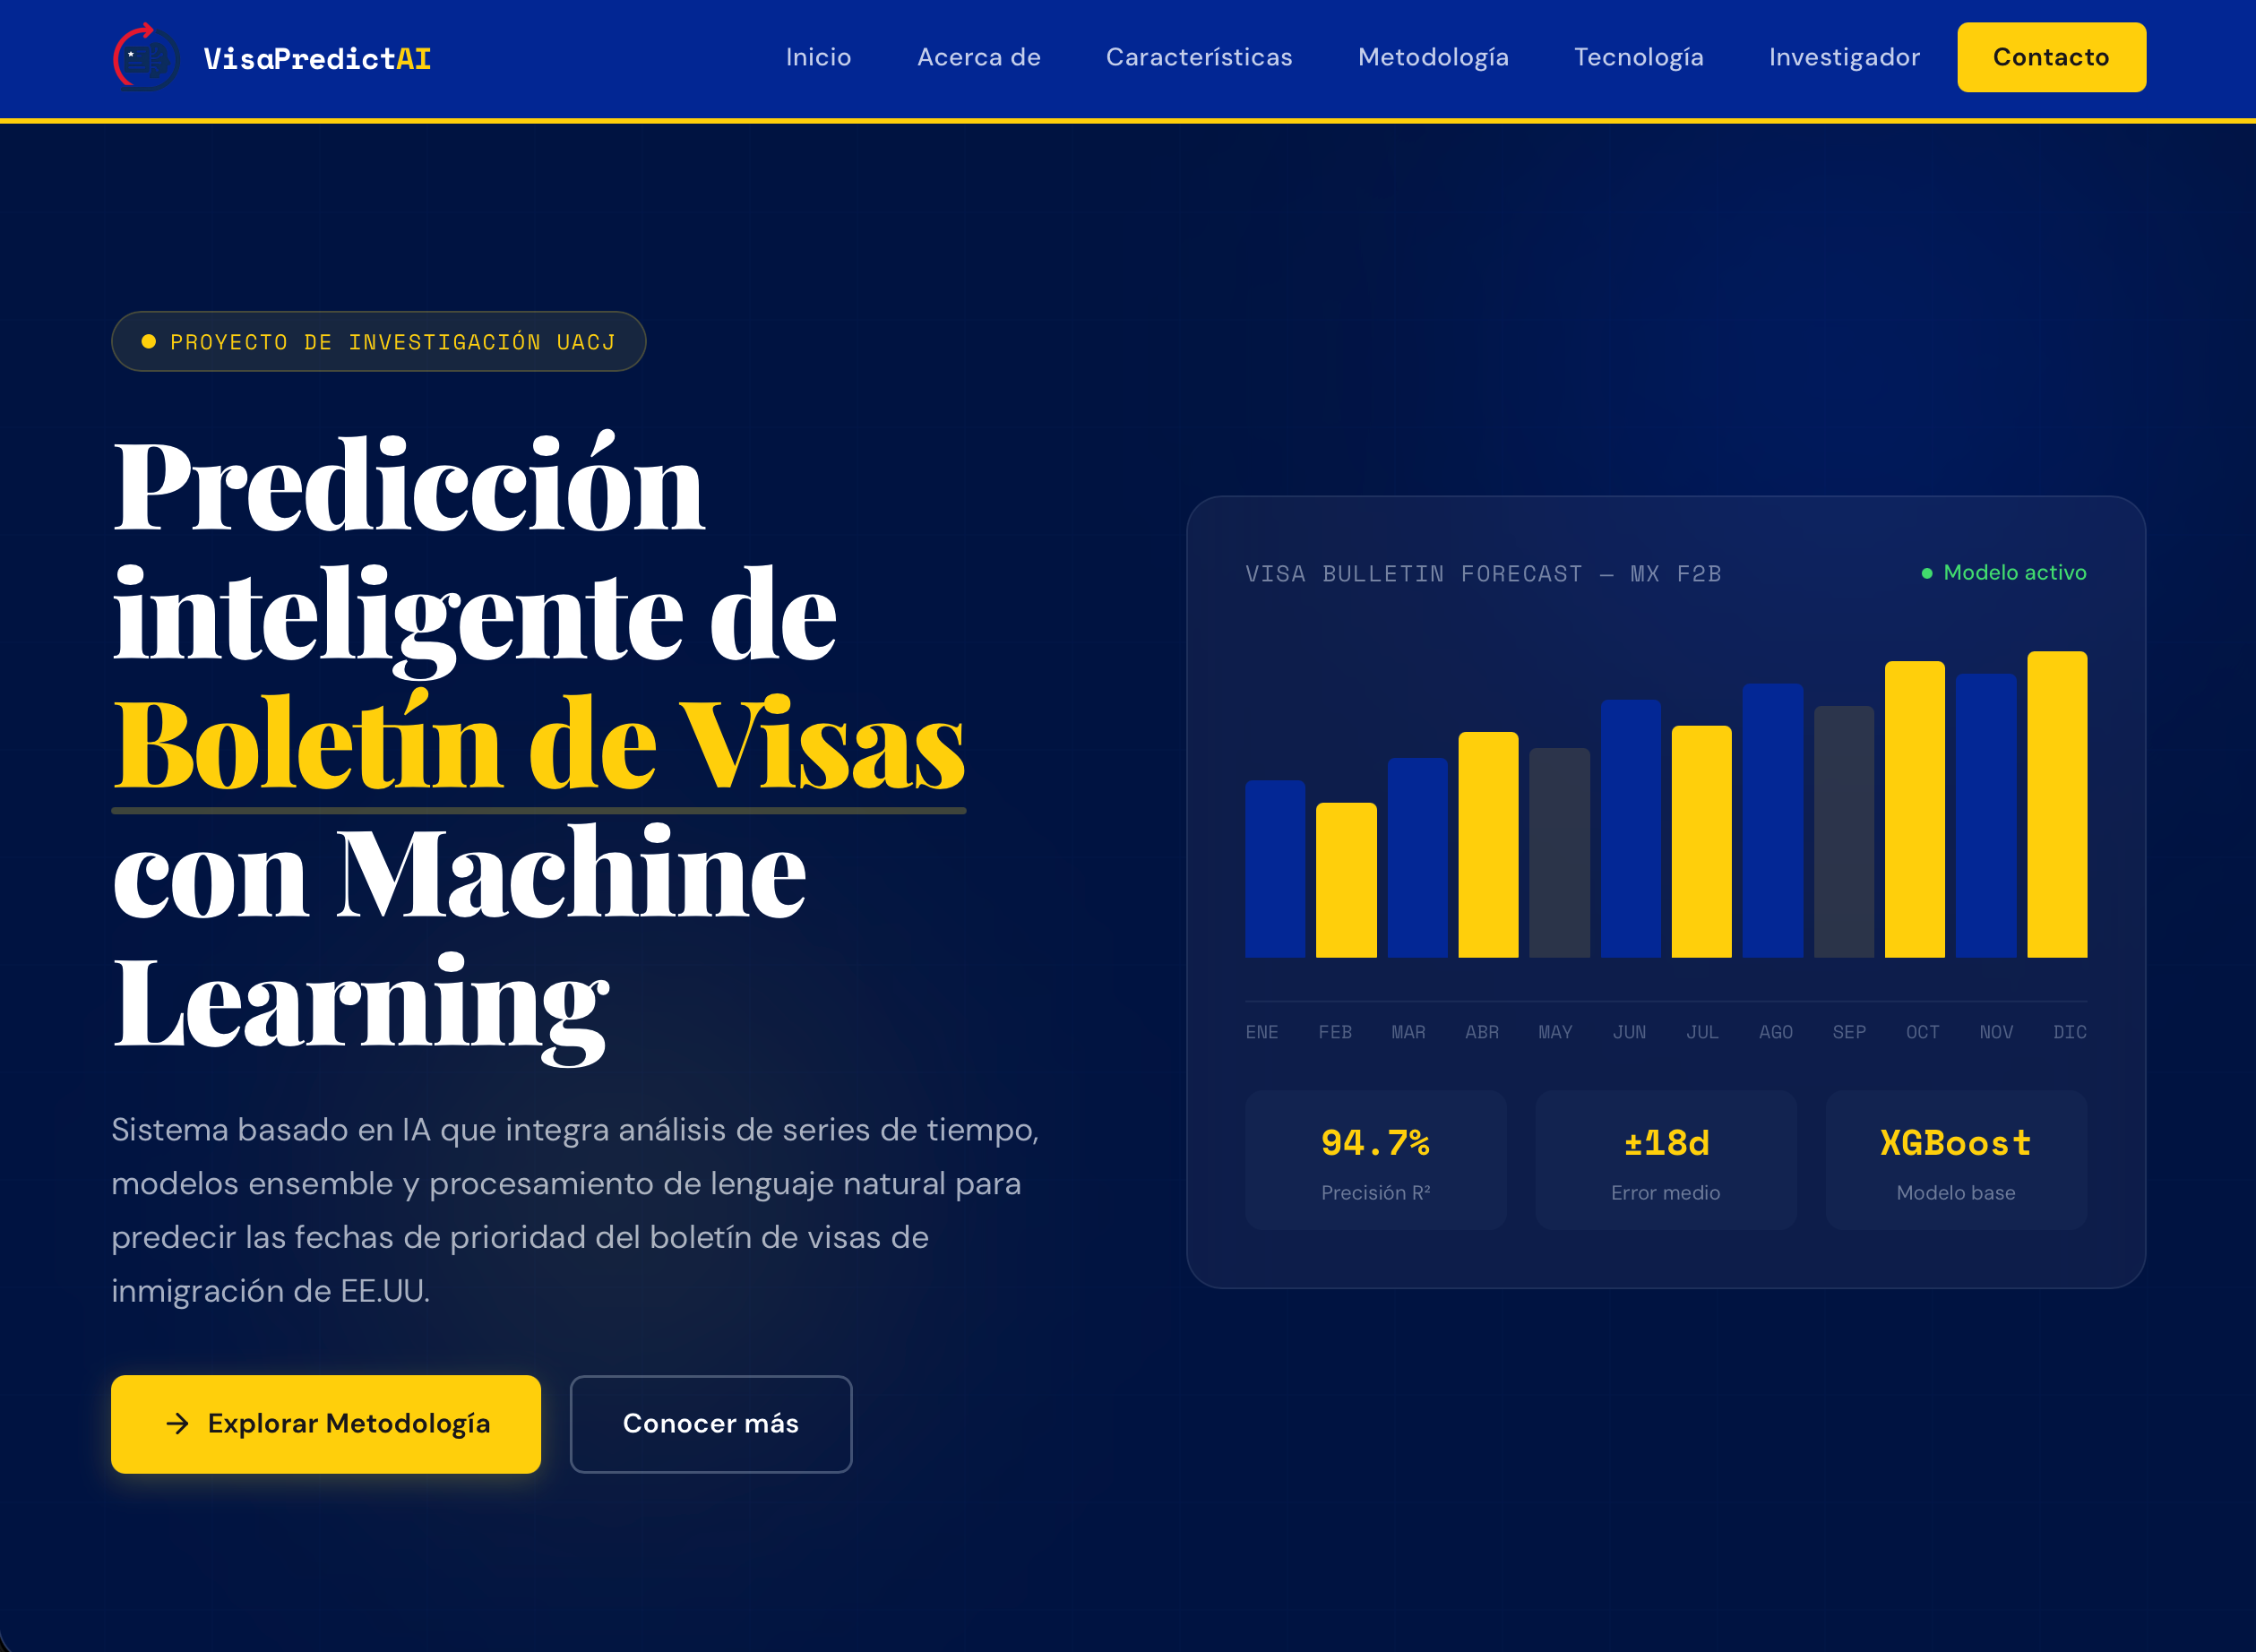
\includegraphics[width=0.78\textwidth]{Visaweb.png}
    \caption[Página de aterrizaje del proyecto personal del autor.]{Página de aterrizaje del proyecto personal del autor (\url{https://visapredictai.com/}). Material descriptivo, \textbf{no parte del entregable académico evaluado}. El demostrador académico oficial se entrega desde el repositorio público (Sección~A.2). Fuente: captura del proyecto personal.}
    \label{fig:portal_visapredict}
\end{figure}

\section{Disclaimer académico versionado}

Toda salida del demostrador académico despliega de manera permanente el siguiente texto, sin posibilidad de ocultarlo en la aplicación:

\begin{quote}
\itshape\small
``Las estimaciones presentadas son producto de un sistema académico de pronóstico basado en datos históricos del U.S.\ Department of State. \textbf{NO} constituyen asesoría legal migratoria, \textbf{NO} predicen el resultado individual de un caso específico y \textbf{NO} garantizan que la fecha real coincida con la estimada. La adjudicación de visas depende de procesos administrativos del USCIS, NVC y consulados, así como de cambios normativos no anticipables por el modelo. El uso de estas estimaciones es exclusivamente informativo. El proyecto no acepta responsabilidad por decisiones individuales (renuncias laborales, compromisos financieros, planes de viaje) tomadas con base en estas predicciones. Los usuarios deben consultar fuentes oficiales (\texttt{travel.state.gov}, \texttt{uscis.gov}) y profesionales legales acreditados para decisiones consecuentes.''
\end{quote}

El texto exacto del \textit{disclaimer} se versiona en el repositorio público bajo \texttt{docs/disclaimer\_academico.txt} y se inyecta automáticamente en toda salida del demostrador. Cualquier modificación queda registrada en el historial de Git, con \textit{commit hash} y fecha.

\clearpage

% ============================================================
% GLOSARIO
% ============================================================
\chapter*{Glosario}
\addcontentsline{toc}{chapter}{Glosario}

\begin{multicols}{2}
\setlength{\columnsep}{14pt}
\scriptsize
\sloppy   % glosario justificado: tolerancia ampliada para columnas estrechas
\hbadness=10000        % silencia underfull \hbox warnings cosméticos
\emergencystretch=3em  % permite mayor margen al algoritmo de saltos de línea
\begin{description}[leftmargin=0pt, labelindent=0pt, itemindent=0pt,
                    labelsep=0.4em, font=\bfseries\scriptsize,
                    itemsep=2pt, parsep=0pt, topsep=0pt]
    \item[ACF] (\textit{Autocorrelation Function})\hspace{0.3em}Función que cuantifica la correlación entre observaciones separadas por distintos rezagos temporales; herramienta central en la identificación de modelos ARIMA.

    \item[Adam] (\textit{Adaptive Moment Estimation})\hspace{0.3em}Algoritmo de optimización de gradiente estocástico que combina momento y tasas de aprendizaje adaptativas por parámetro; estándar \textit{de facto} en entrenamiento de redes profundas.

    \item[AIC] (\textit{Akaike Information Criterion})\hspace{0.3em}Criterio de selección de modelos que balancea ajuste y parsimonia: $\text{AIC} = 2k - 2\ln(\mathcal{L})$.

    \item[ARIMA] (\textit{Autoregressive Integrated Moving Average})\hspace{0.3em}Familia de modelos estadísticos de series de tiempo que combina componentes autorregresivos, de diferenciación y de media móvil para capturar dinámicas lineales.

    \item[ARIMAX] Extensión de ARIMA que incorpora variables exógenas regresoras además de la dinámica endógena de la serie objetivo.

    \item[Backlog (neto)] En el contexto migratorio, volumen acumulado de solicitudes pendientes de procesamiento que excede la capacidad operativa del sistema, medido restando las solicitudes resueltas de las recibidas en un período.

    \item[País de cargabilidad (\textit{chargeability area})] Categoría administrativa bajo la cual el Departamento de Estado contabiliza una solicitud para fines del límite estatutario del 7\,\%. Por defecto coincide con el país de nacimiento del solicitante principal, no con su nacionalidad ni con su país de residencia. Las áreas de cargabilidad reportadas en el \textit{Visa Bulletin} incluyen países individuales (México, India, China, Filipinas, etc.) y la categoría agregada \textit{All Chargeability Areas Except Those Listed}, que NO es un país sino una agrupación residual.

    \item[All Chargeability Areas Except Those Listed] Categoría agregada del \textit{Visa Bulletin} que reúne a todos los países de cargabilidad no listados explícitamente. Es una agrupación administrativa, no una entidad geográfica única; incluye decenas de países de baja a media demanda. Su \textbf{composición varía a lo largo del tiempo} conforme países entran y salen del estado de ``límite efectivo'' por superación de cuota, lo cual constituye una forma de no-estacionariedad de composición. Por esta razón, esta serie se reportará en la cobertura piloto pero será analizada con cautela explícita: cualquier inferencia sobre tendencia se acompañará de la advertencia sobre cambio de composición.

    \item[Nacionalidad vs. país de cargabilidad] Términos no equivalentes en derecho migratorio estadounidense. La cargabilidad sigue, por defecto, al país de nacimiento (INA Sección 202); la nacionalidad del solicitante puede o no coincidir con su país de cargabilidad. Para evitar ambigüedad, el presente documento utiliza consistentemente \textit{país o área de cargabilidad} cuando se refiere a la dimensión $p$ del \textit{Visa Bulletin}.

    \item[Batch Normalization] Técnica de regularización que estandariza las activaciones de una capa al interior de cada minibatch para estabilizar y acelerar el entrenamiento.

    \item[BiLSTM] (\textit{Bidirectional Long Short-Term Memory})\hspace{0.3em}Variante de LSTM que procesa la secuencia simultáneamente en dirección cronológica y anticronológica, permitiendo que cada estado oculto incorpore contexto pasado y futuro.

    \item[DeepAR] Arquitectura probabilística basada en LSTM autorregresiva, diseñada para producir pronósticos de series de tiempo con distribuciones predictivas en lugar de puntos.

    \item[Dates for Filing] Calendario publicado mensualmente por el Departamento de Estado que autoriza el inicio anticipado del trámite de ajuste de estatus, generalmente con fechas más recientes que las \textit{Final Action Dates}.

    \item[Diebold-Mariano (prueba)] Prueba estadística formal de comparación de precisión predictiva entre dos modelos sobre una misma serie, bajo hipótesis nula de igualdad de errores esperados.

    \item[Dropout] Técnica de regularización que desactiva aleatoriamente una fracción de neuronas durante el entrenamiento, forzando redundancia representacional y reduciendo el sobreajuste.

    \item[EB-1 a EB-5] Categorías de preferencia laboral para residencia permanente en EE.\,UU., desde trabajadores prioritarios con habilidades extraordinarias (EB-1) hasta inversionistas (EB-5).

    \item[Early Stopping] Estrategia de regularización implícita que interrumpe el entrenamiento cuando el error sobre el conjunto de validación deja de mejorar durante un número predefinido de épocas.

    \item[F1, F2A, F2B, F3, F4] Categorías de preferencia familiar definidas por la INA: hijos adultos solteros de ciudadanos (F1), cónyuges e hijos menores de residentes (F2A), hijos adultos solteros de residentes (F2B), hijos casados de ciudadanos (F3) y hermanos de ciudadanos (F4).

    \item[Final Action Dates] Fecha de prioridad publicada mensualmente en el \textit{Visa Bulletin} que determina qué solicitantes pueden recibir la adjudicación final de su residencia permanente en ese mes fiscal.

    \item[Gradient Boosting] Familia de métodos de ensamble que construye secuencialmente modelos débiles, cada uno enfocado en corregir los errores residuales del ensamble previo; XGBoost es su implementación más difundida.

    \item[INA] (\textit{Immigration and Nationality Act})\hspace{0.3em}Ley federal estadounidense de 1965 que estableció el sistema actual de cuotas por categoría y país para la residencia permanente.

    \item[LSTM] (\textit{Long Short-Term Memory})\hspace{0.3em}Arquitectura de red neuronal recurrente diseñada por Hochreiter y Schmidhuber en 1997 que incorpora celdas de memoria y compuertas para capturar dependencias temporales de largo plazo y mitigar el desvanecimiento del gradiente.

    \item[MAE] (\textit{Mean Absolute Error})\hspace{0.3em}Error absoluto medio: promedio de los valores absolutos de los errores de predicción.

    \item[MAPE] (\textit{Mean Absolute Percentage Error})\hspace{0.3em}Error porcentual absoluto medio; sensible a valores cercanos a cero y asimétrico entre sobre y subestimaciones.

    \item[MASE] (\textit{Mean Absolute Scaled Error})\hspace{0.3em}Error absoluto escalado medio propuesto por Hyndman y Koehler; métrica universal que normaliza el error por el error del naïve estacional.

    \item[Monte Carlo Dropout] Técnica de cuantificación de incertidumbre que aplica dropout también en inferencia, interpretando las predicciones resultantes como muestras de una distribución predictiva aproximada.

    \item[N-BEATS] (\textit{Neural Basis Expansion Analysis for Time Series})\hspace{0.3em}Arquitectura profunda puramente basada en bloques residuales que ofrece pronósticos interpretables sin recurrir a mecanismos recurrentes.

    \item[PACF] (\textit{Partial Autocorrelation Function})\hspace{0.3em}Función que mide la correlación entre la observación actual y observaciones rezagadas eliminando la influencia lineal de los rezagos intermedios.

    \item[PatchTST] Arquitectura transformer reciente para pronóstico de series largas que segmenta la serie en \textit{patches} temporales tratados como tokens, logrando un rendimiento competitivo con un costo computacional reducido.

    \item[Predicción conforme] (\textit{Conformal Prediction})\hspace{0.3em}Marco no paramétrico introducido por Vovk, Gammerman y Shafer que produce intervalos de predicción con garantías de cobertura válidas bajo el supuesto mínimo de intercambiabilidad de los datos.

    \item[Priority Date] (Fecha de prioridad)\hspace{0.3em}Fecha oficial de registro de una petición migratoria, asignada al recibirse por USCIS o por el Departamento del Trabajo; funciona como turno en la cola de procesamiento.

    \item[Prophet] Biblioteca de pronóstico desarrollada por Meta AI que modela series de tiempo como suma de componentes de tendencia, estacionalidad y efectos de festividades, robusta ante observaciones faltantes y valores atípicos.

    \item[Per-country limit] Límite legal del 7\,\% de las visas de preferencia anuales disponibles para nacionales de un mismo país, origen principal de la severa retrogresión observada en países de alta demanda como México, India, China y Filipinas.

    \item[ReLU] (\textit{Rectified Linear Unit})\hspace{0.3em}Función de activación no lineal $f(x) = \max(0, x)$; de uso dominante en redes profundas modernas por su simplicidad computacional y su mitigación del desvanecimiento del gradiente.

    \item[Retrogresión] Fenómeno del sistema migratorio estadounidense en el que las fechas de prioridad del \textit{Visa Bulletin} retroceden en lugar de avanzar, reflejando un agotamiento anticipado de cuotas o reajustes internos en la asignación de visas.

    \item[RMSE] (\textit{Root Mean Squared Error})\hspace{0.3em}Raíz del error cuadrático medio; métrica sensible a errores grandes por su penalización cuadrática.

    \item[SARIMA] Extensión estacional de ARIMA que incorpora componentes autorregresivos, de diferenciación y de media móvil a nivel estacional con período $s$.

    \item[sMAPE] (\textit{Symmetric Mean Absolute Percentage Error})\hspace{0.3em}Variante simétrica del MAPE que utiliza el promedio de los valores absolutos observados y predichos en el denominador.

    \item[TFT] (\textit{Temporal Fusion Transformer})\hspace{0.3em}Arquitectura híbrida transformer-recurrente para pronóstico multi-horizonte con entradas heterogéneas (pasado, covariables conocidas, variables estáticas).

    \item[\textit{Visa Bulletin}] Boletín mensual publicado por la Oficina de Asuntos Consulares del Departamento de Estado de EE.\,UU. que actualiza las fechas de prioridad para cada categoría migratoria y país.

    \item[Walk-forward Validation] Estrategia de validación para series de tiempo en la que el conjunto de entrenamiento se expande progresivamente hacia el futuro, respetando la causalidad temporal.

    \item[XGBoost] (\textit{eXtreme Gradient Boosting})\hspace{0.3em}Implementación escalable y regularizada de \textit{gradient boosting} sobre árboles de decisión; referente de alto rendimiento en competiciones de aprendizaje automático.
\end{description}
\end{multicols}

\newpage

% ============================================================
% ACERCA DEL AUTOR Y DEL ASESOR DE TESIS
% Versión compacta sin \chapter* (no fuerza pagebreak):
% el bloque continúa a continuación del Glosario en la misma página
% si el espacio remanente lo permite.
% ============================================================
\vspace{0.6cm}
\noindent{\Large\bfseries\textcolor{uacjblue}{Acerca del autor y del asesor}}
\addcontentsline{toc}{chapter}{Acerca del autor y del asesor}
\par\vspace{0.35cm}
\noindent\textcolor{uacjblue}{\rule{\textwidth}{0.6pt}}
\par\vspace{0.35cm}

% ----------------------------- AUTOR -----------------------------
\noindent
\begin{minipage}[t]{0.27\textwidth}
    \vspace{0pt}
    \begin{tikzpicture}
        \clip (0,0) circle (1.55cm);
        \node at (0,0) {
\includegraphics[width=3.1cm]{PROFILE.jpg}};
    \end{tikzpicture}
\end{minipage}%
\hfill
\begin{minipage}[t]{0.70\textwidth}
    \vspace{0pt}
    {\large\bfseries\textcolor{uacjblue}{Javier Augusto Rebull Saucedo}}\\[2pt]
    {\small\itshape\textcolor{uacjgray}{Tesista · MIAAD · UACJ}}\\[4pt]
    \small
    Estudiante de la Maestría en Inteligencia Artificial y Analítica de Datos (MIAAD) de la Universidad Autónoma de Ciudad Juárez (UACJ), con matrícula~263483. En el ámbito profesional se desempeña como \textit{Sr.~Associate Application Developer} en Banco Santander US, con residencia en Boston, Massachusetts, EE.\,UU. Su interés académico se centra en el modelado predictivo de fenómenos sociales con impacto en comunidades migrantes, combinando técnicas de aprendizaje profundo, series de tiempo y analítica de datos aplicada.\\[2pt]
    {\footnotesize $\blacktriangleright$ \href{mailto:al263483@alumnos.uacj.mx}{\texttt{al263483@alumnos.uacj.mx}}}
\end{minipage}

\vspace{0.5cm}

% ----------------------------- ASESOR -----------------------------
\noindent
\begin{minipage}[t]{0.27\textwidth}
    \vspace{0pt}
    \begin{tikzpicture}
        \clip (0,0) circle (1.55cm);
        \node at (0,0) {
\includegraphics[width=3.1cm]{DrVicente.png}};
    \end{tikzpicture}
\end{minipage}%
\hfill
\begin{minipage}[t]{0.70\textwidth}
    \vspace{0pt}
    {\large\bfseries\textcolor{uacjblue}{Dr. Vicente García Jiménez}}\\[2pt]
    {\small\itshape\textcolor{uacjgray}{Director de tesis · UACJ}}\\[4pt]
    \small
    Profesor-investigador del Departamento de Ingeniería Eléctrica y Computación de la Universidad Autónoma de Ciudad Juárez (UACJ) y miembro del núcleo académico del programa de Maestría en Inteligencia Artificial y Analítica de Datos (MIAAD). Su línea de investigación comprende aprendizaje automático aplicado, clasificación con conjuntos desbalanceados y minería de datos. Como asesor de la presente tesis, orienta el diseño metodológico, el rigor experimental y la coherencia teórica del sistema experimental.\\[2pt]
    {\footnotesize $\blacktriangleright$ \href{mailto:vicente.jimenez@uacj.mx}{\texttt{vicente.jimenez@uacj.mx}}}
\end{minipage}

\end{document}
